%-----------------------------------------------------------------------
% Beginning of chap1.tex
%-----------------------------------------------------------------------
%
%  AMS-LaTeX sample file for a chapter of a monograph, to be used with
%  an AMS monograph document class.  This is a data file input by
%  chapter.tex.
%
%  Use this file as a model for a chapter; DO NOT START BY removing its
%  contents and filling in your own text.
% 
%%%%%%%%%%%%%%%%%%%%%%%%%%%%%%%%%%%%%%%%%%%%%%%%%%%%%%%%%%%%%%%%%%%%%%%%

\part{A KAM theorem for $b^m$-symplectic manifolds} 

The KAM theorem explains how integrable systems behave under small perturbations. More precisely, it studies how an integrable system in action-angle coordinates responds to a small perturbation on its Hamiltonian. The trajectories of an integrable system in action-angle coordinates can be seen as linear trajectories over a torus. The KAM theorem finds a way to transform these original trajectories to other linear trajectories over some transformed torus. The KAM theorem states that most of these tori, and the linear solutions of the system on these tori, survive if the perturbation is small enough.


In this part, we give a new KAM theorem for $b^m$-symplectic manifolds with detailed proof. This is contained in the first chapter of this part. 
Moreover, we devote three more chapters to applications:

\begin{enumerate}
\item \textbf{Desingularization of $b^m$-integrable systems.} We present a way to use the desingularization of $b^m$-symplectic manifolds presented in \cite{GMW17} to construct standard smooth integrable systems from $b^m$-integrable systems. This desingularized integrable system is uniquely defined.
\item \textbf{Desingularization of the KAM theorem on $b^m$-symplectic manifolds.} In this section we use the desingularization of $b^m$-integrable systems in conjunction with the KAM theorem for $b^m$-symplectic manifolds to deduce the original KAM theorem as well as a completely new KAM theorem for folded symplectic forms.
\item \textbf{Potential applications to Celestial mechanics.} We overview a list of motivating examples from Celestial mechanics where regularization transformations give rise to $b^m$-symplectic forms. We discuss some potential applications of perturbation theory in this set-up.
 \end{enumerate}
\chapter{A new KAM theorem}


The objective of this chapter is to give a construction of KAM theory in the setting of $b^m$-symplectic manifolds and with $b^m$-integrable systems. The core of the chapter is the construction of the proper statement and the proof of the equivalent of the KAM theorem on $b^m$-symplectic manifolds.


This chapter is  divided different sections:

\begin{enumerate}
\item \textbf{On the structure of the proof.} On this section we are going to present the main ideas that are going to appear in the proper statement and proof of the main theorem. The idea of the theorem is to build a sequence of $b^m$-symplectomorphisms such that its limit transforms the hamiltonian to only depend on the action coordinates.
\item \textbf{Technical results and definitions.} On this section we present some technical results and definitions that are key for the proof of the main theorem.
\item \textbf{KAM theorem on $b^m$-symplectic manifolds.} On this section we present the statement and the proof of the main result of this chapter. The proof is structured in 6 parts. In the first part we define the parameters that are going to be used to define the sequence of $b^m$-symplectomorphisms. In the second part we build precisely this sequence of $b^m$-symplectomorphisms. In the third part we see that the sequence of frequency maps of the transformed Hamiltonian functions at every step converges. In the fourth part we see that the sequence of $b^m$-symplectomorphisms converges. In the fifth part we obtain results on the stability of the trajectories under the original perturbation. In the sixth part, we find bounds to explain how close the invariant tori are from the unperturbed.
Finally, we obtain a bound for the measure of the set of invariant tori.

\end{enumerate}

\section{On the structure of the proof}

The first thing we do is to reduce our study to the case the perturbation is not a $b^m$-function but an analytic one. This is because any purely singular perturbation only affects the component in the direction of the modular vector field and can be easily controlled.

The idea of the proof is really similar to the classical KAM case.
We want to build a diffeomorphism such that its transformed hamiltonian only depends on the action coordinates. But it is not possible to build this diffeomorphism in one step. What we do, as it is done in the classical case, it is to build a sequence of diffeomorphisms such that the part of the hamiltonian depending on the angular variables decreases at every step. The idea is to remove the first $K$ terms of its Fourier expression at every step while making $K$ rapidly increase. This is done by assuming the diffeomorphism comes as the flow at time 1 generated by a Hamiltonian function. In this way one can use the Lie Series in conjunction with the Fourier series to find the expression for the hamiltonian function that generates our diffeomorphism. The final diffeomorphism will be the composition of all the diffeomorphisms obtained at each step. One of the main difficulties of the proof, as in the classical case, is to prove that these diffeomorphisms converge and to prove some bounds of its norm.

We also note that for our $b^m$-symplectic setting, the diffeomorphisms we consider leave the defining function of the critical set invariant up to order $m$, this will have an important role later. Also observe in particular that the critical set can not be transformed by any perturbation given by a $b^m$-function.\\
Next we give some technical definitions and results. We define the norms we are going to use to do all the estimates. We set the notation for the proof and the statement of the theorem. We define the notion of non-resonance for a neighborhood of the critical set of the $b^m$-symplectic manifold. We study the set of all possible non-resonant vectors. And we state the inductive lemma, which gives us estimates and constructions for every step of our sequence of diffeomorphisms.

After all this discussion we are in conditions to properly state the $b^m$-version of the KAM theorem. One important difference to the classical KAM theorem is that we have to guarantee that at $Z$ the set of non-resonant vectors does not become the whole set of frequencies. This condition can be understood as the perturbation being smaller than some constant multiplied by the inverse of the modular period.

The proof of the theorem is done in six different steps by following the structure on \cite{D}. Since we are going to use the inductive lemma at every step, first we define the parameters and sets to which  we are going apply such lemma. Then we check that we can actually apply the lemma and obtain some extra estimates for the results of the lemma. After this we see that the sequence of frequency vectors converges. We do the same with the sequence of canonical transformations. Then we get some bounds for the size of the components of the final diffeomorphism. Next we characterize the tori that survive by the perturbation. Finally we give some estimates for the measure of the set of these tori.

Note that our version of the $b^m$-KAM theorem improves the one in \cite{KMS16} in several ways. Firstly it is applicable to $b^m$-symplectic structures not only for $b$-symplectic. Also we give several estimates that are not obtained in \cite{KMS16}, this estimates have sense in a neighborhood of the critical set $Z$, while \cite{KMS16} only studied the behavior at $Z$. Finally the type of perturbation we consider is far more general, since we do not have any condition of the form of the perturbation but only on its size.


\subsection{Reducing the problem to an analytical perturbation.}

In the standard KAM, we assume to have an analytic Hamiltonian $h(I)$ depending only on the action coordinates and we add to it a small analytical perturbation $R(\phi,I)$. This perturbed system receives the name of \emph{nearly integrable system}. And then find a new coordinate system such that $h(I) + R(\phi,I) = \tilde h(\tilde I)$ where most of the quasi-periodic orbits are preserved and can be mapped to the unperturbed quasi-periodic orbits by means of the coordinate change.

In our setting we may assume $h(I)$ to not be analytical and be a $b^m$-function. Also the  perturbation $R(\phi, I)$ may as well be considered a $b^m$-function. In the following lines we justify without loss of generality that actually we can assume the perturbation to be analytical.

Let us state this more precisely. Let $(M,x,Z,\omega,F)$ be a $b^m$-manifold with a $b^m$ integrable system $F$ on it. Consider action angle coordinates on a neighborhood of $Z$.
Then we can assume the expressions:

$$\omega = \left(\sum_{j=1}^{m}\frac{c_j}{I_1^j}\right) d I_1 \wedge d\phi_1 + \sum_{i=2}^n dI_i\wedge d\phi_i, \text{ and }$$
$$F = (q_0' \log I_1 + \sum_{i=1}^{m-1} q_i'\frac{1}{I_1^i} + h(I), f_2, \ldots, f_n)$$

where $h,f_2,\ldots,f_n$ are analytical.

Let the Hamiltonian function of our system be the first component of the moment map $\hat h' = q'_0\log I_1 + \sum_{i=1}^{m-1} q_i'\frac{1}{I_1^i} + h = \zeta' + h$, where $\zeta' := q_0' \log I_1 + \sum_{i=1}^{m-1} q_i' \frac{1}{I_1^i}$. Note that $d\zeta' = \sum_{i=1}^m \hat q_i'\frac{1}{I_1'}$, where $\hat q_i ' = -(i-1)q_{i-1}'$. Note that by the result of the previous chapter $c_j/\hat q_j ' = \mathcal{K}$ the modular period. In particular $c_m/\hat q_m ' = \mathcal{K}$.

The hamiltonian system given by $\hat h'$ can be easily solved by $\phi = \phi_0 + u' t, I = I_0$ where $u'$ is going to be defined in the following sections.
Consider now a perturbation of this system: $\hat H' = \hat h'(I) = \hat R(I,\phi)$, where $\hat R$ is a $b^m$-function $\hat R(I,\phi) = R_{\zeta}(I_1) + R(I,\phi)$ where $R_\zeta(I_1) = (r_0 \log I_1 + \sum_{i=1}^{m-1} r_i \frac{1}{I_1^i})$ is the singular part. Then we can consider the perturbations $R_\zeta(I_1)$ and $R(I,\phi)$ separately. This way, we may consider $R_\zeta(I)$ as part of $\hat h'(I)$. Then we have a new hamiltonian
$$\hat h(I) = (q_0' + r_0) \log I_1 + \sum_{i=1}^{m-1}(q_i' + r_i)\frac{1}{I_1^i} + h = q_0 \log I_1 + \sum_{i=1}^{m-1} q_i \frac{1}{I_1^i} + h.$$

Now, instead of the identity $\mathcal{K} \hat q_j' = c_j$ we will have $\mathcal{K} (\hat q_j - \hat r_j) = c_j$, which implies $\mathcal{K}\left(1 - \frac{\hat r_j}{\hat q_j ' + \hat r_j}\right) = \frac{c_j}{\hat q_j}$. In particular

$$\mathcal{K}\left(1 - \frac{\hat r_m}{\hat q_m ' + \hat r_m}\right) = \frac{c_m}{\hat q_m}$$

Let us define $\mathcal{K}' = \mathcal{K}\left(1 - \frac{\hat r_m}{\hat q_m ' + \hat r_m}\right)$.
So from now on we assume $\hat h = q_0 \log I_1 + \sum_{i=1}^{m-1} q_i \frac{1}{I_1^i} + h$, that the perturbation $R(\phi,I)$ is analytical, and we have the condition $\frac{c_m}{\hat q_m} = \mathcal{K}'$. Observe that this system with only the singular perturbation is still easy to solve in the same way that the system previous to this perturbation was.

\subsection{Looking for a $b^m$-symplectomorphism}

Assume we have a Hamiltonian function $H = \hat{h}(I) + R(\phi,I)$ in action-angle coordinates. Where $\hat{h}(I)$ is the singular component of the $b^m$-integrable system, i.e.
\begin{equation}\label{eq:bm-hamiltonian}
\hat{h}(I) = h(I) + q_0 \log(I_1) + \sum_{i = 1}^{m-1}q_i\frac{1}{I_1^i},
\end{equation}
where $h(I)$ is analytical\footnote{If another component of the moment map is chosen to be the hamiltonian of the system, the result still holds: the computations can be replicated assuming $\hat{h}(I) = h(I)$.}.
Assume also that the $b^m$-symplectic form $\omega$\footnote{In classical KAM, $\omega$ is used to denote the frequency vector $\frac{\partial h}{\partial I}$. We need $\omega$ to denote the $b^m$-symplectic form so we are going to use $u$ to denote the frequency vector.} in these coordinates is expressed as:
\begin{equation}\label{eq:bm-symplectic}
\omega = \left(\sum_{j = 1}^m\frac{c_{j}}{I_1^j}\right)dI_1\wedge d \phi_1 + \sum_{i=2}^{n}dI_i\wedge d\phi_i.
\end{equation}

And finally, the expression for the frequency vector is:

$$\hat{u} = \frac{\partial \hat{h}}{\partial I} = \frac{\partial(h(I) + q_0 \log(I_1) + \sum_{i = 1}^{m-1}q_i\frac{1}{I_1^i})}{\partial I}$$ $$= \left(u_1 + \sum_{i = 1}^{m}\frac{\hat{q}_i}{I_1^i}, u_2, \ldots, u_n\right),
$$

where $\hat{q}_1 = q_0$ and $\hat{q}_{i-1} = -iq_i$ if $i \neq 0$.

The objective is to follow the steps of the usual KAM construction (the steps followed are highly inspired in \cite{D}) replacing the standard symplectic form for $\omega$ and taking as hamiltonian the $b^m$-function $\hat{h}$.

\begin{remark}
The objective of the construction is to find a diffeomorphism (actually a $b^m$-symplectomorphism) $\psi$ such that $H\circ\psi=h(\tilde{I})$. This is done inductively, by taking $H\circ\psi=H \circ \phi_1\circ\ldots\circ \phi_q \circ\ldots$, while trying to make $R(\phi,I)$ smaller at every step.
\end{remark}

\textbf{Let us focus in one single step}

Recall the classical formula:

\begin{lemma}\label{lemma:lie_taylor} See \cite{D}.
$$f\circ\phi_t=\sum_{j=0}^{\infty}\frac{t^j}{j!}L_W^jf,\quad L_W^jf=\{L_W^{j-1}f,W\}$$
Where $W$ is the Hamiltonian that generates the flow $\phi_t$, and $\{\cdot,\cdot\}$ is the corresponding Poisson bracket.
\end{lemma}

We will denote $r_k(H,W,t)=\sum_{j=k}^\infty\frac{t^j}{j!}L_W^jH$.

\begin{equation}\label{eq:new_hamiltonian_expression}
\begin{array}{rcl}
\displaystyle{H\circ\phi = \left.H\circ\phi\right|_{t=1}}& = & \displaystyle{\sum_{j=0}^{\infty}\frac{t^j}{j!}\left.L_W^j\underbrace{H}_{\hat{h}+R}\right|_{t=1}}\\
\\
&=& \displaystyle{ \hat{h}+R\{\hat{h}+R,W\}+r_2(H,W,1)}\\
\\
&=& \displaystyle{ \hat{h}+R+\{\hat{h},W\}+\{R,W\}+r_2(\hat{h},W,1)}\\
\\
& & \quad \displaystyle{+r_2(R,W,1)}\\
\\
&=& \displaystyle{ \hat{h}+\underbrace{R+\{\hat{h},W\}}_{\begin{subarray}{c}\text{We want to cancel} \\ \text{this term as} \\ \text{fast as we can}\end{subarray}}+r_2(\hat{h},W,1)+r_2(R,W,1)}
\end{array}
\end{equation}

We want $\{\hat{h},W\}+R_{\leq k} =0$, equivalently $\{W,\hat{h}\}= R_{\leq k} $, where $R_{\leq k} $ means the Fourier expression of $R$ up to order $K$:
$$R_{\leq k} = \sum_{\begin{subarray}{c} k\in\mathbb{R}^n \\ |k|_1 \leq K\end{subarray}} R_k(I)e^{ik\cdot\phi}$$

Let us impose the condition $\{W,\hat{h}\}=R_{\leq K}$. Let us write the expression of the Poisson bracket associated to the $b^m$-symplectic form.

$$
\begin{array}{rcl}
\{W,\hat{h}\} & = & \displaystyle \left(\frac{1}{\sum_{j = 1}^m \frac{c_j}{I_1^j}}\right)\left(\frac{\partial W}{\partial \phi_1}\frac{\partial \hat{h}}{\partial I_1} - \frac{\partial W}{\partial I_1}\frac{\partial \hat{h}}{\partial \phi_1}\right)\\
& & + \displaystyle{\sum_{i = 2}^n \left(\frac{\partial W}{\partial \phi_i}\frac{\partial \hat{h}}{\partial I_i} - \frac{\partial W}{\partial I_i}\frac{\partial \hat{h}}{\partial \phi_i}\right)}
\end{array}
$$

%Using the two expanded expressions:

%$$
%\begin{array}{rcl}
% \displaystyle{\sum_{i = 2}^n \left(\frac{\partial W}{\partial \phi_i}\frac{\partial h}{\partial I_i} - \frac{\partial W}{\partial I_i}\frac{\partial h}{\partial \phi_i}\right)} + I_1^m\left(\frac{\partial W}{\partial \phi_i}\frac{\partial h}{\partial I_i} - \frac{\partial W}{\partial I_i}\frac{\partial h}{\partial \phi_i}\right) & = & \displaystyle{\sum_{\begin{subarray}{c} k\in\mathbb{R}^n \\ |k|_1 \leq K\end{subarray}} R_k(I)e^{ik\cdot\phi}}
%\end{array}
%$$

Because $\hat{h}$ depends only on $I$, $\frac{\partial \hat{h}}{\partial \phi_i} = 0$ for all $i$. Moreover, the singular part of the $b^m$-function only depends on $I_1$ and hence its derivatives with respect to the other variables are also 0. Using that $\frac{\partial \hat{h}}{\partial I} = u + \sum_{i = 1}^{m}\frac{\hat{q}_i}{I_1^i}$ the previous expression can be  simplified:

$$
\begin{array}{rcl}
\{W,\hat{h}\} & = & \displaystyle \left(\frac{u_1 + \sum_{i = 1}^{m}\frac{\hat{q}_i}{I_1^i}}{\sum_{j = 1}^m \frac{c_j}{I_1^j}}\right)\frac{\partial W}{\partial \phi_1} + \displaystyle\sum_{i = 2}^n \frac{\partial W}{\partial \phi_i}u_i
\end{array}
$$

To expand the expression further we develop $W$ in its Fourier expression: $W=\sum_{\begin{subarray}{c} k\in\mathbb{R}^n \\ |k|_1 \leq K\end{subarray}}W_k(I)e^{ik\phi}$. The Fourier expansion is added up to order $K$, because it is only necessary for the expressions to agree up to order $K$. With this notations the condition becomes:

\begin{longtable}{rcl}
$\{W,\hat{h}\}_{\leq K}$ & $=$ & $\displaystyle
 \left(\frac{u_1 + \sum_{i = 1}^{m}\frac{\hat{q}_i}{I_1^i}}{\sum_{j = 1}^m \frac{c_j}{I_1^j}}\right)\frac{\partial }{\partial \phi_1}\left(\sum_{\begin{subarray}{c} k\in\mathbb{R}^n \\ |k|_1 \leq K\end{subarray}}W_k(I)e^{ik\phi}\right)$\\
 \\
& & $\qquad \qquad \qquad  + \displaystyle\sum_{j = 2}^n u_j \frac{\partial }{\partial \phi_j}\left(\sum_{\begin{subarray}{c} k\in\mathbb{R}^n \\ |k|_1 \leq K\end{subarray}}W_k(I)e^{ik\phi}\right)$\\
\\
& $=$ & $\displaystyle\left(\frac{u_1 + \sum_{i = 1}^{m}\frac{\hat{q}_i}{I_1^i}}{\sum_{j = 1}^m \frac{c_j}{I_1^j}}\right)\left(\sum_{\begin{subarray}{c} k\in\mathbb{R}^n \\ |k|_1 \leq K\end{subarray}}W_k(I)e^{ik\phi}ik_1\right)$\\
\\
& &  $\qquad \qquad \qquad + \displaystyle\sum_{j = 2}^n u_j \left(\sum_{\begin{subarray}{c} k\in\mathbb{R}^n \\ |k|_1 \leq K\end{subarray}}W_k(I)e^{ik\phi}ik_j\right)$
\\
\\
& = & $\displaystyle \sum_{\begin{subarray}{c} k\in\mathbb{R}^n \\ |k|_1 \leq K\end{subarray}} W_k(I)e^{ik\phi}\cdot\left( i k_1 \left(\frac{u_1 + \sum_{i = 1}^{m}\frac{\hat{q}_i}{I_1^i}}{\sum_{j = 1}^m \frac{c_j}{I_1^j}}\right)
+ \sum_{j=2}^nik_ju_j\right)$\\
\\
$ = R_{\leq K}$\\
\end{longtable}
Then, it is possible to make the two sides of the equation equal by imposing the condition term by term:

\begin{equation}\label{eq:solve_coefs}
\begin{array}{rcl}
W_k(I) & = & \displaystyle R_k(I)\frac{1}{i\left(k_1 \left(\frac{u_1 + \sum_{i = 1}^{m}\frac{\hat{q}_i}{I_1^i}}{\sum_{j = 1}^m \frac{c_j}{I_1^j}}\right)  + \sum_{j = 2}^n k_ju_j\right)}
\\
\\
& = & \displaystyle R_k(I)\frac{1}{i\left(k_1 \left(\frac{u_1 + \sum_{i = 1}^{m}\frac{\hat{q}_i}{I_1^i}}{\sum_{j = 1}^m \frac{c_j}{I_1^j}}\right) + \bar{k}\bar{u}\right)},
\end{array}
\end{equation}

where we adopted the notation $\sum_{j = 2}^n k_ju_j = \bar{k}\bar{u}$.

\begin{remark}
Observe that the expression \ref{eq:solve_coefs} has no sense when $k = \vec{0}$ and hence $\{W,h\}_0=R_0$\footnote{The zero term of the Fourier series can be seen as the angular average of the function} can not be solved. Let $W_0(I)=0$, then $\{h,W\}_{\leq K} = R_{\leq K} -R_0$.
\end{remark}

Plugging the results above into the equation  \ref{eq:new_hamiltonian_expression}, one obtains:

$$
H\circ\phi = \hat{h}  + R_0 + R_{\geq K} + r_2(\hat{h},W,1) + r_1(R,W,1)
$$

With this construction the diffeomorphism $\phi$ is found. But this is  only the first of many steps. If $q$ denotes the number of the iteration of this procedure, in general, we obtain:

\begin{equation}
\begin{array}{rcl}
H^{(q)}  =  H^{(q-1)}\circ\phi^{(q)} & = &  \hat{h}^{(q-1)}  + R_0^{(q-1)} + R_{\geq K}^{(q-1)} \\
& & + r_2(h^{(q-1)},W^{(q)},1) + r_1(R^{(q-1)},W^{(q)},1),
\end{array}
\end{equation}

and at every step:

\begin{equation}\label{eq:iterative_h_and_R}
\begin{cases}
\hat{h}^{(q)}  =  \hat{h}^{(q-1)} + R_0^{(q-1)}\\
R^{(q)}  =  R_{>K}^{(q-1)} + r_2(\hat{h}^{(q-1)}, W^{(q)},1) + r_1(R^{(q-1)}, W^{(q)},1)\\
\end{cases}
\end{equation}

\subsection{On the change of the defining function under \\ $b^m$-symplectomorphisms}

Note that since we are considering $b^m$-manifolds it only makes sense to consider $I_1$ up to order $m$, see \cite{Scott16}. When talking about defining functions we are interested in $[I_1]$, its jet up to order $m$.
By definition $b^m$-maps preserve $I_1$ up to order $m$ and $b^m$-vector fields $X$ are such that $\mathcal{L}_X(I_1) = g\cdot I_1^m$ for $g\in\mathcal{C}^\infty(M)$.

\begin{lemma}
Let $\phi_t$ be the integral flow of $X$ a $b^m$-vector field, then $\phi_t$ is a $b^m$-map.
\end{lemma}
\begin{proof}
We want
$$I_1\circ \phi_t = I_1 + I_1^m\cdot g$$ for some $g\in \mathcal{C}^\infty(M)$.
We will use \ref{lemma:lie_taylor}.
$$I_1 \circ \phi_t = \sum_{j=0}^\infty \frac{t^j}{j!}L_X^j I_1 = I_1 + \mathcal{L}_X(I_1) + \sum_{j=2}^\infty\frac{t^j}{j!}L_X^j I_1$$
$$= I_1 +  I_1^m + \sum_{j=2}^\infty\frac{t^j}{j!}L_X^j I_1.$$
On the other hand, let us prove by induction $L_X^k I_1 = g^{(k)} I_1^m$. The first case is obvious, assume the case $k$ holds and let us prove the case $k+1$.

$$
\begin{array}{rcl}
L_X^{k+1} I_1 & = & \{L_X^k I_1, X\} \\
& = & \{g^{(k)} I_1^m, X\} \\
& = & (L_X g^{(q)}) I_1^m + g^{(k)}\cdot m I_1^{m-1}L_X I_1 \\
& = & (L_X g^{(k)} + g^{(k)}\cdot m \cdot I_1^{m-1}\cdot g) I_1^m \\
& = & g^{(k+1)} I_1^m \\
\end{array}
$$

where $g^{(k+1)} = L_X g^{(k)} + g^{(k)}\cdot m \cdot I_1^{m-1}\cdot g$.

\end{proof}

\begin{lemma}
The Hamiltonian vector flow of some smooth hamiltonian function $h$ is a $b^m$-vector field.
\end{lemma}
\begin{proof}
At each point of $Z$ the following identity holds $\mathcal{L}_{X_h} I_1 = I_1^m\frac{\partial f}{\partial \phi_1}$. The result can be extended at a neighborhood of $Z$.
\end{proof}

Observe that combining the two previous results we get that the hamiltonian flow of a function preserves $I_1$ up to order $m$.


%A $b^m$-symplectomorphism must preserve the defining function of the critical set $Z$ by definition, but we are going to the check that actually the $b^m$-symplectomorphisms defined above send $I_1$ to $I_1$ which is more demanding than just leaving $Z$ invariant. Which is actually true because we are considering the analytic version.


%Let $h$ be any $b^m$-function $h = q_0 \log I_1 + \sum_{i=1}^{m-1} q_i \frac{1}{I_1^i} + f$, $q_0 \in \mathbb{R}$, $q_i \in \mathcal{C}^\infty(I_1)$ if $i \geq 2$.
%In this more general case $\hat q_i = -(i-1)q_{i-1} + \partial(q_i)/\partial I_1$.
%Then,
%$$dh = \sum_{i=1}^m \frac{\hat q_i}{I_1^i} dI_1 + \sum_{i=1}^m \frac{\partial f}{\partial I_i} dI_i + \sum_{i= 1}^m \frac{\partial f}{\partial \phi_i} d\phi_i.$$
%Assume also,
%$$\Pi = \frac{1}{\sum_{i=1}^m\frac{c_i}{I_1^i}}\frac{\partial}{\partial I_1}\wedge\frac{\partial}{\partial \phi_1} + \sum_{j=2}^n \frac{\partial}{\partial I_j}\wedge\frac{\partial}{\partial \phi_j}.$$
%With this equation we can compute
%$$X_h = \Pi(dh,\cdot) = \frac{\sum_{i=1}^m \frac{\hat q_i}{I_1^i}}{\sum_{i=1}^m \frac{c_i}{I_1^i}}\frac{\partial}{\partial \phi_1} + \frac{\frac{\partial f}{\partial I_i}}{\sum_{i=1}^m \frac{c_i}{I_1^i}}\frac{\partial}{\partial \phi_1} - \frac{\frac{\partial f}{\partial \phi_1}}{\sum_{i=1}^m \frac{c_i}{I_1^i}}\frac{\partial}{\partial I_1} + \sum_{j=2}^{n}\frac{\partial f}{\partial I_j}\frac{\partial }{\partial \phi_j} + \sum_{j=2}^{n}\frac{\partial f}{\partial \phi_j}\frac{\partial}{\partial I_j}$$


%We can use formula \ref{lemma:lie_taylor} to see if the function $I_1$ is preserved by the diffeomorphism generated by $X_h$. We have to check that $L_h^q I_1 = 0$ at $Z$ for all $q \geq 1$.

%$$L_h^1 I_1 = \{I_1,h\} = -X_h\cdot I_1 = \frac{\frac{\partial f}{\partial \phi_1}}{\sum_{i=1}^m\frac{c_i}{I_1^i}}.$$

%Which vanishes at $Z$. Moreover,

%$$
%\begin{array}{rcl}
%L_h^2 I_1 = \{L_h^1, h\} = -X_h\cdot L_h^1 I_1 &=& -\frac{\sum_{i=1}^m\frac{\hat q_1}{I_1^i}}{(\sum_{i=1}^m\frac{c_i}{I_1^i})^2}\frac{\partial^2 f}{\partial \phi_1^2} - \frac{\frac{\partial f}{\partial I_1}\frac{\partial^2 f}{\partial \phi^2}}{\sum_{i=1}^m \frac{c_i}{I_1^i})^2}\\
% & & \quad +  \frac{\frac{\partial f}{\partial \phi_1}}{\sum_{i=1}^m \frac{c_i}{I_1^i}}\frac{\frac{\partial^2 f}{\partial \phi_1 \partial I_1}(\sum_{i=1}^m \frac{c_i}{I_1^i}) + \frac{\partial f}{\partial \phi_1}(\sum_{i=1}^{m} (-i\frac{c_i}{I_1^{i+1}}))}{(\sum_{i=1}^m \frac{c_i}{I_1^i})^2}\\
% & & \quad + \sum_{j=2}^n \frac{\partial f}{\partial I_j} \frac{\frac{\partial^2 f}{\partial\phi_1 \phi_j}}{\sum_{i=1}^m \frac{c_i}{I_1^i}} + \sum_{j=2}^n \frac{\partial f}{\partial \phi_j} \frac{\frac{\partial^2 f}{\partial\phi_1 I_j}}{\sum_{i=1}^m \frac{c_i}{I_1^i}}.\\
%\end{array}
%$$

%This way it is easy to prove by induction that every time we iterate $L_h^q I_1$ the maximum degree of the denominators increase faster than the maximum degree of the numerators. Thus this shows what we wanted.

%\begin{remark}
%Since the diffeomorphisms leave $I_1$ invariant they will also leave $\zeta$ invariant, hence the singular part of the hamiltonian will not be modified by the diffeomorphisms outlined above.
%\end{remark}


\section{Technical results}


As the non-singular part of our functions we will be considering analytic functions on $\mathbb{T}\times G$, $G \subset \mathbb{R}^n$. The easiest way to work with these functions is to consider them as holomorphic functions on some complex neighborhood. Let us define formally this neighborhood.

$$\mathcal{W}_{\rho_1}(\mathbb{T}^n) := \{ \phi : \Re\phi \in \mathbb{T}^n, |\Im \phi|_{\infty} \leq \rho_1\},$$
$$\mathcal{V}_{\rho_2}(G) := \{I \in \mathbb{C}^n : |I - I'|\leq \rho_2 \text{ for some } I' \in G\},$$
$$\mathcal{D}_\rho (G) := \mathcal{W}_{\rho_1}(\mathbb{T}^n) \times \mathcal{V}_{\rho_2}(G),$$

where $|\cdot|_\infty$ denotes the maximum norm and $|\cdot|_2$ denotes de Euclidean norm.
Now it is necessary to clarify the norms that are going to be used on these sets.

\begin{definition}
Let $f$ be an action function (only depending on the $I$-coordinates), and $F$ an action vector field.
$$
\begin{array}{rl}
|f|_{G,\eta} := \sup_{I\in\mathcal{V}_\eta(G)} |f(I)|,  & |f|_G := |f|_{G,0}\\
|F|_{G,\eta,p} := \sup_{I\in\mathcal{V}_\eta(G)} |F(I)|_p,  & |F|_{G,\eta} := |F|_{G,\eta,2}\\

\end{array}
$$
Now, assume $f(I,\phi)$ to be an action-angle function written using its Fourier expansion as $\sum_{k\in\mathbb{Z}^n} f_k(I)e^{ik\cdot\phi}$, and $F$ to be an action-angle vector field.
$$
\begin{array}{rcl}
|f|_{G,\rho} := \sup_{(\phi,I)\in\mathcal{D}_\rho(G)} |f(I)|, & \|f\|_{G,\rho}:=\sum_{k\in\mathbb{Z}^n} |f_k|_{G,\rho_2} e^{|k|_1\rho_1}\\
|F|_{G,\rho,p} := \sum_{k\in\mathbb{Z}^n} |F_k|_{G,\rho_2,p} e^{|k|_1\rho_1}, & \|F\|_{G,\rho} = \|F\|_{G,\rho,2}\\
\end{array}
$$
\end{definition}

\begin{lemma}[Cauchy Inequality]
$$\left\|\frac{\partial f}{\partial \phi}\right\|_{G,(\rho_1-\delta_1, \rho_2),1}\leq \frac{1}{e\delta_1}\left\|f\right\|_{G,\rho}$$
$$\left\|\frac{\partial f}{\partial I}\right\|_{G,(\rho_1, \rho_2-\delta_2),\infty}\leq \frac{1}{\delta_2}\|f\|_{G,\rho}$$
\end{lemma}

\begin{definition}
If $Df=(\frac{\partial f}{\partial \phi}, \frac{\partial f}{\partial I})$,
$$\|Df\|_{G,\rho,c}:= \max\left(\|\frac{\partial f}{\partial \phi}\|_{G,\rho,1},c\|\frac{\partial f}{\partial I}\|_{G,\rho,\infty}\right)$$
\end{definition}

\begin{definition}To simplify our notation, let us define:
$$\mathcal{A}(I_1) = \frac{\sum_{j = 1}^{m}\frac{\hat{q}_j}{I_1^j}}{\sum_{j=1}^m \frac{c_j}{I_1^j}} \quad \text{ and } \quad \mathcal{B}(I_1) = \frac{1}{\sum_{j=1}^m \frac{c_j}{I_1^j}}.$$
\end{definition}

\begin{remark}
With this notation, equation \ref{eq:solve_coefs} can be written as:
$$W_k(I) = \frac{R_k(I)}{i(k_1 \mathcal{B}(I_1) u_1 + \bar{k}\bar{u} + k_1 \mathcal{A}(I_1))}$$
\end{remark}



Observe that $\mathcal{A}(I_1)$ and $\mathcal{B}(I_1)$ are analytic (holomorphic on the complex extended domain) where the denominator does not vanish. We can assume that this does not happen by shrinking the domain $G$ in the direction of $I_1$. Observe, in particular, that when $I_1 \rightarrow 0$, $\mathcal{A}(I_1) \rightarrow \hat q_m/c_m = 1/\mathcal{K}'$ the inverse of the modular period and $\mathcal{B}(I_1) \rightarrow 0$. In this way,  the norms of $\mathcal{A}(I_1)$ and $\mathcal{B}(I_1)$ are bounded and well defined. We will denote these norms by $K_{\mathcal{A}}$ and $K_{\mathcal{B}}$ respectively. Also, since $\mathcal{A}(I_1)$ and $\mathcal{B}(I_1)$ are analytic, their derivatives will also be bounded, and we will denote the norms of these derivatives by $K_{\mathcal{A}'}$ and $K_{\mathcal{B}'}$.


To further simplify  the notation in the following computations we introduce the definition:

\begin{definition}

$$
\bar{\mathcal{A}} = \left(\begin{array}{c}
\mathcal{A}\\
0 \\
\end{array}\right)
\quad \text{ and } \quad
\bar{\mathcal{B}} = \left(\begin{array}{cc}
\mathcal{B} & 0\\
0 & \text{Id}_{n-1,n-1}\\
\end{array}\right)
$$

\end{definition}

\begin{remark}
With this notation, equation \ref{eq:solve_coefs} can be written as:
\begin{equation}\label{eq:solve_coefs_simplified}
W_k(I) = \frac{R_k(I)}{i(k \bar{\mathcal{B}}(I_1) u + k \bar{\mathcal{A}}(I_1))}
\end{equation}


\end{remark}

\begin{definition}
Having fixed $\omega$, a $b^m$-symplectic form (as in equation \ref{eq:bm-symplectic}) and $\hat{h}$ a $b^m$-function (as in equation \ref{eq:bm-hamiltonian}) as a hamiltonian. Given an integer $K$ and $\alpha > 0$, $F \subset \mathbb{R}^n$ (or $\mathbb{C}^n$) the space of frequencies is said to be $\alpha, K$-non-resonant with respect to $(c_1,\ldots,c_m)$ and $(\hat{q}_1,\ldots, \hat{q}_m)$ if
$$|k \bar{\mathcal{B}}(I_1) u + k \bar{\mathcal{A}}(I_1)|\geq \alpha, \forall k \in \mathbb{Z}\setminus \{0\}, |k|_1\leq K, \forall u \in F.$$
We are going to use the notation $\alpha, K, c,\hat{q}$-non-resonant.
\end{definition}



\begin{remark}
The non-resonance condition is established on $u = \partial h/\partial I$, not on $\hat{u} = \partial \hat h/\partial I$, because our non-resonance condition already takes into account the singularities. In this way we can use the analytic character of $u$.
\end{remark}

\begin{remark}
If $\left|\frac{\partial u}{\partial I}\right|_{G,\rho_2}$ is bounded by $M'$,  then $\left|\frac{\partial }{\partial I}\left( \bar{\mathcal{B}}u + \bar{\mathcal{A}}\right)\right|_{G,\rho_2}$ is also bounded:

\begin{equation}\label{eq:M_def}
\begin{array}{rcl}
\left|\frac{\partial }{\partial I}\left( \bar{\mathcal{B}}u + \bar{\mathcal{A}}\right)\right|_{G,\rho_2} &
 \leq &
 \left|\frac{\partial \bar{\mathcal{B}}}{\partial I} u
  + \bar{\mathcal{B}} \frac{\partial u}{\partial I}
   + \frac{\partial \bar{\mathcal{A}}}{\partial I}\right|_{G,\rho_2}\\
\\
& \leq & K_{\mathcal{B}'} |u|_{G,\rho_2} + K_{\mathcal{B}}M' + K_{\mathcal{A}} =: M.\\
\\
\end{array}
\end{equation}

\end{remark}

\begin{remark}
When we consider the standard KAM theorem, the frequency vector $u$ is relevant because the solution to the Hamilton equations of the unperturbed problem has the form:

$$I = I_0, \quad \phi = \phi_0 + ut.$$

Let us see what plays the role of $u$ in our $b^m$-KAM theorem. Let us find the coordinate expression of the solution to $\iota_{X_{\hat{h}}} \omega=  d \hat{h}$, where $\omega$ is a $b^m$-symplectic form in action-angle coordinates.

$$X_{\hat{h}} = \dot{I}_1\frac{\partial}{\partial I_1} + \ldots + \dot{I}_n\frac{\partial}{\partial I_n},$$

where $\dot{I}_1,\ldots, \dot{I}_n$ are the functions we want to find.

$$d\hat{h} = \left(\sum_{j=1}^m \hat{q}_i \frac{1}{I_1^j}\right) dI_1 + dh,$$

and hence,

$$X_{\hat{h}} = \Pi(d \hat{h},\cdot ) = \frac{\sum_{i=1}^m \frac{\hat q_i}{I_1^i}}{\sum_{i=1}^m \frac{c_j}{I_1^j}}\frac{\partial}{\partial \phi_i} + X_h.$$

Hence $\phi = \phi_0 + (\underbrace{\bar{\mathcal{B}} u + \bar{\mathcal{A}}}_{u'})t$. So the frequency vector that we are going to be concerned about is going to be $u'$ instead of $\hat{u} = \frac{\partial}{\partial I} \hat{h}$.
\end{remark}
\begin{lemma}
If $u$ is one-to-one from $\mathcal{G}$ to its image then $u' = \bar{\mathcal{B}} u + \bar{\mathcal{A}}$ is also one-to-one from $\mathcal{G}'$ to its image in a neighborhood of $Z$, while at $Z$ it is the projection of $u$ such that the first coordinate is sent to $\frac{\hat q_m}{c_m} = 1/\mathcal{K}'$ the inverse of the modular period, were  $\mathcal{G}'\subseteq \mathcal{G}$.
\end{lemma}
\begin{proof}
Because $$u' = \left(\frac{1}{\sum_{j=1}^m \frac{c_j}{I_1^j}} u_1 + \frac{\sum_{j=1}^m \frac{\hat{q}_j}{I_1^j}}{\sum_{j=1}^m \frac{c_j}{I_1}},u_2,\ldots,u_n\right),$$
and  $\mathcal{B}$ is invertible outside $I_1 = 0$, shrinking $\mathcal{G}$ if necessary in the first dimension the map is one-to-one. But at the critical set $\{I_1 = 0\}$, $u'$ is a projection of $u$ where the first component is sent to the constant value $\frac{\hat q_m}{c_m} = \frac{1}{\mathcal{K}'}$.
\end{proof}
\begin{lemma}
If $u(G)$ is $\alpha,K, c,\hat{q}$-non-resonant, then $u(\mathcal{V}_{\rho_2}(G))$ is $\frac{\alpha}{2},K, c,\hat{q}$-non-resonant, assuming that $\rho_2\leq \frac{\alpha}{2MK}$ and $\left|\frac{\partial u}{\partial I}\right|_{G,\rho_2} \leq M'$
\end{lemma}
\begin{proof}
Fix $k\in\mathbb{Z}\setminus\{0\}$, we want to bound $|k \bar{\mathcal{B}}(I_1) v + k \bar{\mathcal{A}}(I_1)|$ where $v\in u(\mathcal{V}_{\rho_2}(G))$ as a function on $v$.
Given $v \in u(\mathcal{V}_{\rho_2}(G))$ we  ask whether there is any bound for the distance to some $v'\in u(G)$.
$$v \in u(\mathcal{V}_{\rho_2}(G)) \Rightarrow v = u(x), x \in \mathcal{V}_{\rho_2}(G)\Rightarrow\exists y \in G \text{ such that } |x-y| \leq \rho_2.$$
Take $v'=u(y)$.


$$|v-v'|\leq|x-y|\left|\frac{\partial u}{\partial I}\right|_{G,\rho_2} \leq \rho_2 M' \leq \rho_2  M/K_\mathcal{B} \leq \frac{\alpha}{2MK} M/K_\mathcal{B} = \frac{\alpha}{2K K_\mathcal{B}}.$$

Where we used equation \ref{eq:M_def} in the third inequality.

$$
\begin{array}{rcl}
\displaystyle |k_1 \mathcal{B}(I_1) v_1 + \bar{k}\bar{v} + k_1 \mathcal{A}(I_1)| & \geq & \displaystyle \underbrace{|k_1 \mathcal{B}(I_1) v'_1 + \bar{k}\bar{v'} + k_1 \mathcal{A}(I_1)|}_{\geq \alpha} \\
& & -|k_1 \mathcal{B}(I_1) (v_1-v'_1) + \bar{k}(\bar{v} - \bar{v}')|\\
\\
& \geq & \displaystyle \alpha - K_\mathcal{B}\underbrace{|k\cdot(v-v')|}_{\leq K \alpha /(2K K_\mathcal{B})} \\
\\
 & \geq & \alpha -\alpha/2 = \alpha/2
\end{array}
$$

\end{proof}

\begin{proposition}\label{prop:14}
Let $\hat{h}(I)$ be a $b^m$-function as in equation \ref{eq:bm-hamiltonian}. Assume $h(I)$ and $R(\phi, I)$ be real analytic on $\mathcal{D}_\rho(G)$, $u(G) = \frac{\partial h}{\partial I}(G)$ is $\alpha, K, c, \hat{q}$-non-resonant.
Assume also that
$|\frac{\partial}{\partial I} u|_{G,\rho_2} \leq M'$
and $\rho_2 \leq \frac{\alpha}{2MK}$. Let $c > 0$ given.
Then $R_0(\phi, I)$, $W_{\leq K}(\phi, I)$ given by the previous construction are both real analytic on $\mathcal{D}_\rho(G)$ and the following bounds hold
\begin{enumerate}
\item\label{prop:14:item:1} $||D R_0||_{G,\rho,c} \leq ||D R||_{G,\rho,c}$
\item\label{prop:14:item:2} $||D (R - R_0)||_{G,\rho,c} \leq ||D R_0||_{G,\rho,c}$
\item\label{prop:14:item:3} $||D W||_{G,\rho,c} \leq \frac{2A}{\alpha}||D R_0||_{G,\rho,c}$
\end{enumerate}
Where $A = 1 + \frac{2Mc}{\alpha}$
\end{proposition}

\begin{proof}
Inequalities \ref{prop:14:item:1} and \ref{prop:14:item:2} are obvious because of the Fourier expression.
Let us prove inequality \ref{prop:14:item:3}. Let us expand $R(\phi,I)$ and $W(\phi, I)$ in their Fourier expression:
$$R = \sum_{\begin{subarray}{c} k\in\mathbb{R}^n\end{subarray}} R_k(I)e^{ik\cdot\phi}, \quad W = \sum_{\begin{subarray}{c} k\in\mathbb{R}^n \end{subarray}} W_k(I)e^{ik\cdot\phi}.$$
We will bound this expression finding  term-by-term bounds.

$$\frac{\partial R}{\partial \phi} = \sum_{\begin{subarray}{c} k\in\mathbb{R}^n\end{subarray}} R_k(I)e^{ik\cdot\phi}ik.$$

Hence, if we denote  $[ \frac{\partial R}{\partial \phi} ]_k $ the $k$-th term of the Fourier expansion of $\frac{\partial R}{\partial \phi}$, we have:

$$\left[ \frac{\partial R}{\partial \phi} \right]_k = R_k ik.$$

Let us compute the derivative of $W_k$ with respect to the $I$ variables:

\begin{longtable}{rcl}
$\displaystyle \frac{\partial W_k}{\partial I}$ & $=$ & $\displaystyle\frac{\partial}{\partial I}\left(\frac{R_k}{i(k \bar{\mathcal{B}}(I_1) u  + k \bar{\mathcal{A}}(I_1))}\right)$\\
\\
& $=$ & $\displaystyle \frac{\partial R_k/\partial I }{i(k \bar{\mathcal{B}}(I_1) u  + k \bar{\mathcal{A}}(I_1)))} - \frac{R_k i \frac{\partial}{\partial I }(k \bar{\mathcal{B}}(I_1) u  + k \bar{\mathcal{A}}(I_1)))}{[i(k \bar{\mathcal{B}}(I_1) u  + k \bar{\mathcal{A}}(I_1)))]^2}$\\
\\
& $=$ & $\displaystyle \frac{\partial R_k/\partial I }{i(k \bar{\mathcal{B}}(I_1) u  + k \bar{\mathcal{A}}(I_1)))} + \frac{R_k i k \frac{\partial}{\partial I }(\bar{\mathcal{B}}(I_1) u  + \bar{\mathcal{A}}(I_1)))}{[(k \bar{\mathcal{B}}(I_1) u  + k \bar{\mathcal{A}}(I_1)))]^2}$\\
\\
& $=$ & $\displaystyle \frac{\partial R_k/\partial I }{i(k \bar{\mathcal{B}}(I_1) u  + k \bar{\mathcal{A}}(I_1)))} + \frac{[\frac{\partial R_k}{\partial \phi}]_k \frac{\partial}{\partial I }(\bar{\mathcal{B}}(I_1) u  + \bar{\mathcal{A}}(I_1)))}{[(k \bar{\mathcal{B}}(I_1) u  + k \bar{\mathcal{A}}(I_1)))]^2}.$\\
\end{longtable}


Then, we take norms ($|\cdot|_{G,\rho_2,\infty}$) on each side of the equation.

$$
\begin{array}{rcl}
\displaystyle \left|\frac{\partial W_k}{\partial I}\right|_{G,\rho_2, \infty} & \leq & \displaystyle \frac{2}{\alpha}\left|\frac{\partial R_k}{\partial I}\right|_{G,\rho_2, \infty} +
\displaystyle \frac{4M}{\alpha^2}\left|\left[\frac{\partial R_k}{\partial \phi}\right]_k\right|_{G,\rho_2, \infty}\\
\\
& \leq & \displaystyle \frac{2}{\alpha}\left|\frac{\partial R_k}{\partial I}\right|_{G,\rho_2, \infty} +
\displaystyle \frac{4M}{\alpha^2}\left|\left[\frac{\partial R_k}{\partial \phi}\right]_k\right|_{G,\rho_2, 1}.
\end{array}
$$

Taking the supremum at the whole domain:

$$
\begin{array}{rcl}
\displaystyle \left\|\frac{\partial W_k}{\partial I}\right\|_{G,\rho_2, \infty} & \leq & \displaystyle \frac{2}{\alpha}\left\|\frac{\partial R_k}{\partial I}\right\|_{G,\rho_2, \infty} +
\displaystyle \frac{4M}{\alpha^2}\left\|\left[\frac{\partial R_k}{\partial \phi}\right]_k\right\|_{G,\rho_2, 1}.
\end{array}
$$

Moreover,

$$
\begin{array}{rcl}
\displaystyle \frac{\partial W(I)}{\partial \phi} & = & \displaystyle \frac{\partial}{\partial \phi}\left(\sum_{\begin{subarray}{c} k\in\mathbb{R}^n \end{subarray}} W_k(I)e^{ik\cdot\phi}\right)\\
\\
 & = & \displaystyle \frac{\partial}{\partial \phi}\left(\sum_{\begin{subarray}{c} k\in\mathbb{R}^n \end{subarray}} ik W_k(I)e^{ik\cdot\phi}\right).\\
\end{array}
$$

Hence, the $k$-th term of the Fourier series of $\frac{\partial W}{\partial \phi}$ is

$$\left[\frac{\partial W}{\partial \phi}\right]_k = W_k ik = \frac{R_k}{i(k \bar{\mathcal{B}}(I_1) u  + k \bar{\mathcal{A}}(I_1)))}ik $$
$$= \frac{1}{i(k \bar{\mathcal{B}}(I_1) u  + k \bar{\mathcal{A}}(I_1)))}\left[\frac{\partial R}{\partial \phi}\right]_k.$$

Taking norms ($\|\cdot\|_{G,\rho,1}$) at each side:

$$ \left\|\frac{\partial W}{\partial \phi}\right\|_{G,\rho,1} \leq \frac{2}{\alpha}\left\|\frac{\partial W}{\partial \phi}\right\|_{G,\rho,1}.$$

Then,


\begin{longtable}{rcl}
$\displaystyle \left\|D W\right\|_{G,\rho, c}$ & $=$ & $\displaystyle \max\left(\left\|\frac{\partial W}{\partial \phi}\right\|_{G,\rho,1}, c\left\|\frac{\partial W}{\partial I}\right\|_{G,\rho,\infty}\right)$\\
\\
& $\leq$ & $\displaystyle \max\left(\frac{2}{\alpha}\left\|\frac{\partial R}{\partial \phi}\right\|_{G,\rho,1}, c  \frac{2}{\alpha}\left\|\frac{\partial R}{\partial I}\right\|_{G,\rho_2, \infty} +
c\frac{4M}{\alpha^2}\left\|\frac{\partial R}{\partial \phi}\right\|_{G,\rho_2, 1} \right)$\\
\\
& $\leq$ & $\displaystyle \max\left(\frac{2}{\alpha}\left\|\frac{\partial R}{\partial \phi}\right\|_{G,\rho,1}, \frac{2}{\alpha}\left\|DR\right\|_{G,\rho_2, c} +
c \frac{4M}{\alpha^2}\left\| DR\right\|_{G,\rho_2, c} \right)$\\
\\
& $=$ & $\displaystyle \max\left(\frac{2}{\alpha}\left\|\frac{\partial R}{\partial \phi}\right\|_{G,\rho,1}, \frac{2}{\alpha}\left(1 + \frac{2M}{\alpha}c\right)\left\| DR\right\|_{G,\rho_2, c} \right)$\\
\\
& $\leq$ & $\displaystyle \frac{2}{\alpha}\left(1 + \frac{2M}{\alpha}c\right)\left\| DR\right\|_{G,\rho_2, c}$\\
\\
& $\leq$ & $\displaystyle \frac{2}{\alpha}A\left\| DR\right\|_{G,\rho_2, c}$,\\
\end{longtable}


where $A$ is as desired.


\end{proof}

Recall the Cauchy inequalities, see \cite{JP93}:

\begin{equation}\label{eq:cauchy_ineq}
\begin{array}{llr}
\displaystyle \left\|\frac{\partial f}{\partial \phi}\right\|_{G,(\rho_1, \rho_2),1} & \leq & \displaystyle \frac{1}{e \delta_1}\|f\|_{G,\rho} \\
\displaystyle \left\|\frac{\partial f}{\partial I}\right\|_{G,(\rho_1, \rho_2-\delta_2),\infty}& \leq & \displaystyle \frac{1}{\delta_2}\|f\|_{G,\rho}
\end{array}
\end{equation}

\begin{lemma}\label{lemma:1.1}
Let $f,g$ be analytic functions on $\mathcal{D}_\rho(G)$, where
$0<\delta = (\delta_1, \delta_2) < \rho = (\rho_1, \rho_2)$ and $c > 0$.
Define $\hat\delta_c := \min(c\delta_1, \delta_2)$. The following inequalities hold:
\begin{enumerate}
\item $\|Df\|_{G,\rho- \delta,c} \leq \frac{c}{\hat\delta_c}\|f\|_{G,\rho}$
\item $\|\{f,g\}\|_{G,\rho}\leq \frac{2}{c}\|Df\|_{G,\rho, c}\cdot \|D g\|_{G, \rho,c}$
\item $\|D(f_{>K})\|_{G, (\rho-\delta_1, \rho_2),c} \leq e^{-K\delta_1}\|Df\|_{G,\rho, c}$
\end{enumerate}
\end{lemma}

\begin{proof}
Let us prove each point separately.
\begin{enumerate}
\item %$$\|Df\|_{G,\rho-\delta, c} = \max \left\{\left\|\frac{\partial f}{\partial \phi}\right\|_{G,\rho-\delta, 1}, c\left\|\frac{\partial f}{\partial I}\right\|_{G,\rho-\delta,\infty}\right\}$$

Using the Cauchy inequalities one obtains the following:
$$\left\|\frac{\partial f}{\partial \phi}\right\|_{G,\rho-\delta,1} = \left\|\frac{\partial f}{\partial \phi}\right\|_{G,(\rho_1-\delta_1, \rho_2- \delta_2), 1} $$
$$\leq \left\|\frac{\partial f}{\partial \phi}\right\|_{G,(\rho_1-\delta_1, \rho_2), 1} \leq \frac{1}{e\delta_1} \|f\|_{G,\rho},$$
$$\left\|\frac{\partial f}{\partial I}\right\|_{G,\rho-\delta,\infty} = \left\|\frac{\partial f}{\partial I}\right\|_{G,(\rho_1-\delta_1, \rho_2- \delta_2), \infty} $$
$$\leq \left\|\frac{\partial f}{\partial I}\right\|_{G,(\rho_1, \rho_2-\delta_2), \infty} \leq \frac{1}{\delta_1} \|f\|_{G,\rho}.$$
Putting the two inequalities inside the definition of the norm:
$$
\begin{array}{rcl}
\|D f\|_{G,\rho-\delta, c} &=& \displaystyle \max\left\{\left\|\frac{\partial f}{\partial \phi}\right\|_{G,\rho-\delta, 1}, c\left\|\frac{\partial f}{\partial I}\right\|_{G, \rho-\delta, \infty}\right\} \\
\\
& \leq & \displaystyle \max \left\{\frac{1}{e \delta_1}\|f\|_{G,\rho}, \frac{c}{\delta_2}\|f\|_{G, \rho}\right\}\\
\\
& \leq & \displaystyle \max \left\{\frac{1}{e\delta_1}\frac{c}{c}, \frac{c}{\delta_2}\right\}\|f\|_{G,\rho}\\
\\
& \leq & \displaystyle \max \left\{\frac{c}{e \hat\delta_c},\frac{c}{\hat\delta_c}\right\}\|f\|_{G,\rho},\\
\end{array}
$$

where the last inequality holds because $\hat\delta_c = \min(c\delta_1,\delta_2)$.

\item
Let us find the expression of $\{f,g\}$ for a $b^m$-symplectic structure.
$\{f,g\} = \omega(X_f, X_g)$ where $X_f$ and $X_g$ are such that $\iota_{X_f}\omega=df$ and $\iota_{X_g}\omega=dg$. Let restrict the computations only to $f$.
$$df = \sum_{i=1}^n\frac{\partial f}{\partial \phi_1}d\phi_1, \quad X_f = \sum_{i= 1}^n a_i \frac{\partial}{\partial \phi_i} + \sum_{i=1}^n b_i \frac{\partial}{\partial \phi_i}.$$

Where $a_i$ and $b_i$ are coefficients to be determined by imposing the following condition:

$$\iota_{X_f}\omega = \left(\sum_{j=1}^m\frac{c_j}{ I_1^j}\right)(a_1 dI_1 - b_1 d\phi_1) + \sum_{i = 2}^n (a_i dI_i - b_i d\phi_i) = df.$$

Then, solving for the coefficients the following expressions are obtained:

$$a_1  = \frac{1}{\left(\sum_{j=1}^m\frac{c_j}{ I_1^j}\right)}\frac{\partial f}{\partial \phi_1} \quad \text{and} \quad a_i = \frac{\partial f}{\partial \phi_i} \text{ for } i \neq 1,$$
$$b_1  = -\frac{1}{\left(\sum_{j=1}^m\frac{c_j}{ I_1^j}\right)}\frac{\partial f}{\partial \phi_1} \quad \text{and} \quad b_i = -\frac{\partial f}{\partial \phi_i} \text{ for } i \neq 1.$$

Hence, the expression for the hamiltonian vector fields becomes:

$$
X_f = \frac{1}{\left(\sum_{j=1}^m\frac{c_j}{ I_1^j}\right)}\left(\frac{\partial f}{\partial \phi_1}\frac{\partial }{\partial \phi_1}- \frac{\partial f}{\partial I_1}\frac{\partial }{\partial I_1}\right) + \sum_{i = 1}^n\left(\frac{\partial f}{\partial \phi_i}\frac{\partial }{\partial \phi_i}- \frac{\partial f}{\partial I_i}\frac{\partial }{\partial I_i}\right),$$
$$
X_g =  \frac{1}{\left(\sum_{j=1}^m\frac{c_j}{ I_1^j}\right)}\left(\frac{\partial g}{\partial \phi_1}\frac{\partial }{\partial \phi_1}- \frac{\partial g}{\partial I_1}\frac{\partial }{\partial I_1}\right) + \sum_{i = 1}^n\left(\frac{\partial g}{\partial \phi_i}\frac{\partial }{\partial \phi_i}- \frac{\partial g}{\partial I_i}\frac{\partial }{\partial I_i}\right).
$$

Then the Poisson bracket applied to the two functions:

$$
\begin{array}{rcl}
\{f,g\}=\omega(X_f,X_g) & = & \displaystyle \frac{1}{\left(\sum_{j=1}^m\frac{c_j}{ I_1^j}\right)}\left(\frac{\partial f}{\partial I_1}\frac{\partial g}{\partial \phi_1} - \frac{\partial f}{\partial \phi_1}\frac{\partial g}{\partial I_1}\right)
\\
& & \displaystyle \quad + \sum_{i = 2}^n \left(\frac{\partial f}{\partial I_i}\frac{\partial g}{\partial \phi_i} - \frac{\partial f}{\partial \phi_i}\frac{\partial g}{\partial I_i}\right).
\end{array}
$$

And hence the norm of the Poisson bracket becomes:

$$
\begin{array}{rcl}
\|\{f,g\}\|_{G, \rho} & = & \displaystyle \left\|\frac{1}{\left(\sum_{j=1}^m\frac{c_j}{ I_1^j}\right)}\left(\frac{\partial f}{\partial I_1}\frac{\partial g}{\partial \phi_1} - \frac{\partial f}{\partial \phi_1}\frac{\partial g}{\partial I_1}\right)\right. \\
& & \quad \displaystyle+ \left.\sum_{i = 2}^n \left(\frac{\partial f}{\partial I_i}\frac{\partial g}{\partial \phi_i} - \frac{\partial f}{\partial \phi_i}\frac{\partial g}{\partial I_i}\right) \right\|_{G, \rho} \\
& \leq & \displaystyle \left\|\sum_{i = 1}^n \left(\frac{\partial f}{\partial I_i}\frac{\partial g}{\partial \phi_i} - \frac{\partial f}{\partial \phi_i}\frac{\partial g}{\partial I_i}\right) \right\|_{G, \rho} \\
\end{array}
$$

Where we assumed $\left|\sum_{j=1}^m\frac{c_j}{ I_1^j}\right| \geq 1$. This assumption makes sense, because we are interested in the behaviour close the critical set $Z$. Close enough to the critical set this expression holds. Then,

\begin{longtable}{rcl}
$\|\{f,g\}\|_{G, \rho}$ & $\leq$ & $\displaystyle \sum_{i = 1}^n \left\|\frac{\partial f}{\partial I_i}\right\|_{G, \rho}\left\|\frac{\partial g}{\partial \phi_i}\right\|_{G, \rho} +\sum_{i = 1}^n \left\|\frac{\partial f}{\partial \phi_i}\right\|_{G, \rho}\left\|\frac{\partial g}{\partial I_i}\right\|_{G, \rho}$\\
\\
& $\leq$ & $\displaystyle \left|\frac{\partial f}{\partial I}\right|_{G,\rho,\infty} \left|\frac{\partial g}{\partial I}\right|_{G,\rho,1} + \left|\frac{\partial f}{\partial I}\right|_{G,\rho,1} \left|\frac{\partial g}{\partial I}\right|_{G,\rho,\infty}$\\
\\
& $\leq$ & $\displaystyle \frac{1}{c}|Df\|_{G,\rho,c}\|Dg\|_{G,\rho,c} + \frac{1}{c}|Df\|_{G,\rho,c}\|Dg\|_{G,\rho,c}$\\
\\
& $\leq$ & $\displaystyle \frac{2}{c}\|Df\|_{G,\rho,c}\|Dg\|_{G,\rho,c}.$
\end{longtable}


\item Lastly,

$$
\left\|D(f_{>K})\right\|_{G,(\rho_1 - \delta_1,\rho_2),1} $$
$$= \max \left\{ \left\|\frac{\partial f_{>K}}{\partial \phi}\right\|_{G, (\rho_1-\delta_1, \rho_1), 1}, c\left\|\frac{\partial f_{>K}}{\partial I}\right\|_{G, (\rho_1-\delta_1, \rho_1), \infty}\right\}.
$$

We will proceed by bounding each term separately. On one hand:

\begin{longtable}{rcl}
$\displaystyle\left\|\frac{\partial f}{\partial \phi}\right\|_{G,(\rho_1,\rho_2),1}$ & $=$ & $\displaystyle \left\|\sum_{k\in\mathbb{Z}^n} ikf_k(I)e^{ik\phi}\right\|_{G,(\rho_1,\rho_2),1}$\\
\\
& $\geq$ & $\displaystyle \sum_{k\in\mathbb{Z}^n} k\left\|f_k(I)\right\|_{G,\rho_2,1}e^{|k|_1\rho_1}$\\
\\
& $\geq$ & $\displaystyle \sum_{\substack{k\in\mathbb{Z}^n \\ |k|_1 > K}} k\left\|f_k(I)\right\|_{G,\rho_2,1}e^{|k|_1(\rho_1 + \delta_1 - \delta_1)}$\\
\\
& $\geq$ & $\displaystyle e^{K \delta_1}\sum_{\substack{k\in\mathbb{Z}^n \\ |k|_1 > K}} k\left\|f_k(I)\right\|_{G,\rho_2,1}e^{|k|_1(\rho_1 - \delta_1)}$\\
\\
& $=$ & $\displaystyle e^{K \delta_1}\left\|\frac{\partial f_{>K}}{\partial \phi}\right\|_{G,(\rho_1-\delta_1,\rho_2),1}.$\\
\end{longtable}


On the other hand:

\begin{longtable}{rcl}
$\displaystyle \left\|\frac{\partial f}{\partial I}\right\|_{G,(\rho_1,\rho_2),\infty}$& $=$ & $\displaystyle \left\|\sum_{k \in \mathbb{Z}^n} \frac{\partial f_k(I)}{\partial I} e^{ik\phi}\right\|_{G,(\rho_1,\rho_2),\infty}$\\
\\
& $\geq$ & $\displaystyle \sum_{k \in \mathbb{Z}^n} \left\|\frac{\partial f_k(I)}{\partial I}\right\|_{G,\rho_2,\infty} e^{|k|_1\rho_1}$ \\
\\
& $\geq$ & $\displaystyle \sum_{\substack{k\in\mathbb{Z}^n \\ |k|_1 > K}} \left\|\frac{\partial f_k(I)}{\partial I}\right\|_{G,\rho_2,\infty} e^{|k|_1(\rho_1 + \delta_1 - \delta_1)}$ \\
\\
& $\geq$ & $\displaystyle e^{K\delta_1}\sum_{\substack{k\in\mathbb{Z}^n \\ |k|_1 > K}} \left\|\frac{\partial f_k(I)}{\partial I}\right\|_{G,\rho_2,\infty} e^{|k|_1(\rho_1 - \delta_1)}$\\
\\
& $\geq$ & $\displaystyle e^{K\delta_1}\left\|\frac{\partial f_{>K}}{\partial I}\right\|_{G,(\rho_1-\delta_1,\rho_2),\infty}.$\\
\end{longtable}


Hence $\|D(f_{>k})\|_{G,(\rho_1-\delta_1,\rho_2),c} \leq e^{-K\delta_1}\|Df\|_{G,\rho,c}$.

\end{enumerate}
\end{proof}

Now we define a norm that indicates how close a map $\Phi$ is to the identity.

\begin{definition}
Let $x = (\phi,I) \in \mathbb{C}^{2n}$, then
$$|x|_c := \max(|\phi|_1, c|I|_\infty)$$
\end{definition}

\begin{definition}
For a map $\Upsilon :\mathcal{D}_\rho(G)\rightarrow \mathbb{C}^{2n}$ its norm and the norm of its derivative its defined as:
$$ |\Upsilon|_{G,\rho,c}:=\sup_{x\in\mathcal{D}_\rho(G)}|\Upsilon(x)|_c,$$
$$ |D\Upsilon|_{G,\rho,c}:=\sup_{x\in\mathcal{D}_\rho(G)}|D\Upsilon(x)|_c,$$

where $\displaystyle |D\Upsilon(x)|_c = \sup_{\substack{y\in\mathbb{R}^{2n} \\ |y|_c = 1}}|D\Upsilon(x)\cdot y|_c$
\end{definition}

\begin{lemma}
If $\Upsilon$ is analytic on $\mathcal{D}_\rho(G)$, then $|D\Upsilon|_{G,\rho-\delta,C} \leq \frac{|\Upsilon|_{G,\rho,c}}{\hat\delta_c}$
\end{lemma}


\begin{proof}
Observe that if we consider $\|.\|$ any norm on $\mathbb{C}^n$ and a matrix $A$ of size $n\times n$, and $\|A\|$ defines the induced norm of matrices  i.e.
$$\|A\| = \sup_{\substack{y\in\mathbb{C}^{2n} \\ \|y\| = 1}}\|A\cdot y\|$$
then one has that $\|(\|a_1\|',\ldots,\|a_n\|')\| \leq \|A\|$ where $a_j$ denotes the $j$-th row of $A$. Also note that $\|\cdot\|'$ can be a any norm consider the infinity norm. This can be easily proven in the following way:
$$\|A\cdot y\| = \left\|\left(\begin{array}{c}a_1\cdot y \\ \vdots \\ a_n\cdot y\end{array}\right)\right\| \leq \left\|\left(\begin{array}{c}
\|a_1\|'\|y\|' \\ \vdots \\ \|a_n\|'\|y\|'
\end{array}\right)\right\|$$
Where $\forall y \in \mathbb{C}^n \text{ such that } \|y\| = 1$.
Let $a_j$ be the rows of $D\Upsilon(x)$,
$$ a_j = \left(\frac{\partial \Upsilon_j}{\partial \phi},\frac{\partial \Upsilon j}{\partial I}\right),$$
and be $\|a_j\|'$ its norm.
With this property in mind we proceed as follows:
\begin{longtable}{rcl}
$|D\Upsilon|_{G,\rho-\delta,c}$ & $=$ & $\displaystyle\sup_{x\in \mathcal{D}_{\rho-\delta}(G)} |D\Upsilon(x)|_c$ \\
\\
& $\leq$ & $\displaystyle\sup_{x\in \mathcal{D}_{\rho-\delta}(G)} |(|a_1|_\infty,\ldots,|a_n|_\infty)|_c$\\
%\\
%& $\leq$ & $ \left|\left(\max\left(\sup_{x\in\mathcal{D}_{\rho-\delta}}\left|\frac{\partial \Upsilon_1}{\partial \phi}\right|_1, c\sup_{x\in\mathcal{D}_{\rho-\delta}}\left|\frac{\partial \Upsilon_1}{\partial I}\right|_\infty\right),\ldots\right.\right.$\\
%\\
%& & $\qquad\left.\left.\ldots,\max\left(\sup_{x\in\mathcal{D}_{\rho-\delta}}\left|\frac{\partial \Upsilon_{2n}}{\partial \phi}\right|_1, c\sup_{x\in\mathcal{D}_{\rho-\delta}}\left|\frac{\partial \Upsilon_{2n}}{\partial I}\right|_\infty\right)\right)\right|_c$\\
%\\
%& $=$ & $ \left|\left(\max\left(\left\|\frac{\partial \Upsilon_1}{\partial \phi}\right\|_{G,\rho-\delta,1}, c\left\|\frac{\partial \Upsilon_1}{\partial I}\right\|_{G,\rho-\delta,\infty}\right),\ldots\right.\right.$\\
%\\
%& & $\qquad\left.\left.\ldots,\max\left(\left\|\frac{\partial \Upsilon_{2n}}{\partial \phi}\right\|_{G,\rho-\delta,1}, c\left\|\frac{\partial \Upsilon_{2n}}{\partial I}\right\|_{G,\rho-\delta,\infty}\right)\right)\right|_c$\\

\\
& $\leq$ & $ \left|\left(\sup_{x\in \mathcal{D}_{\rho-\delta}}\left\|D \Upsilon_1\right\|_{\infty},\ldots,\sup_{x\in \mathcal{D}_{\rho-\delta}} \left\|D \Upsilon_{2n}\right\|_{\infty}\right)\right|_c$\\
\\
& $=$ & $ \left|\left(\left\|D \Upsilon_1\right\|_{G,\rho-\delta,\infty},\ldots,\left\|D \Upsilon_{2n}\right\|_{G,\rho-\delta,\infty}\right)\right|_c$\\
\\
& $\leq$ & $ \left|\left(\frac{1}{\delta_1}\left\| \Upsilon_1\right\|_{G,\rho},\ldots,\frac{1}{\delta_1}\left\| \Upsilon_{2n}\right\|_{G,\rho}\right)\right|_c$\\
%\\
%& $\leq$ & $ \left|\left(\max\left(\frac{c}{e\hat\delta_c}\left\| \Upsilon_1\right\|_{G,\rho}, \frac{c}{\hat\delta_c}\left\| \Upsilon_1\right\|_{G,\rho}\right),\ldots\right.\right.$\\
%\\
%& & $\qquad\left.\left.\ldots,\max\left(\frac{c}{e\hat\delta_c}\left\| \Upsilon_{2n}\right\|_{G,\rho}, \frac{c}{\hat\delta_c}\left\| \Upsilon_{2n}\right\|_{G,\rho}\right)\right)\right|_c$\\
%\\
%& $\leq$ & $\left|\frac{c}{\hat\delta_c}\left\|\Upsilon_1\right\|_{G,\rho},\ldots,\frac{c}{\hat\delta_c}\left\|\Upsilon_{2n}\right\|_{G,\rho}\right|_c$\\
\\
& $\leq$ & $\frac{1}{\hat\delta_c}\left|\left\|\Upsilon_1\right\|_{G,\rho},\ldots,\left\|\Upsilon_{2n}\right\|_{G,\rho}\right|_c$\\
\\
& $=$ & $\frac{1}{\hat\delta_c}\sup_{x\in\mathcal{D}_\rho(G)}\left|\Upsilon_1,\ldots,\Upsilon_{2n}\right|_c = \frac{1}{\hat\delta_c}\sup_{x\in\mathcal{D}_\rho(G)}\left|\Upsilon\right|_c$\\
\\
& $=$ & $ \frac{1}{\hat\delta_c}\left|\Upsilon\right|_{G,\rho,c}$\\

\end{longtable}


\end{proof}

\begin{lemma}\label{lemma:1.2} Let $W$ be an analytic function on $\mathcal{D}_\rho(G)$, $\rho > 0$ and let $\Phi_t$ be its Hamiltonian flow at time $t$ ($t>0$). Let $\delta=(\delta_1,\delta_2)>0$ and $c>0$ given. Assume that $\|DW\|_{G,\rho,c}\leq \hat\delta_c$. Then, $\Phi_t$ maps $\mathcal{D}_{\rho-t\delta}(G)$ into $\mathcal{D}_{\rho}(G)$ and one has:
\begin{enumerate}
\item $|\Phi_t-\id|_{G,\rho-t\delta,c}\leq t \|DW\|_{G,\rho,c}$,
\item $\Phi(\mathcal{D}_{\rho}(G)) \supset \mathcal{D}_{\rho-t\delta}(G)$ for $\rho'\leq \rho-t\delta$,
\item Assuming that $\|DW\|_{G,\rho,c} < \hat\delta_c/2e$, for any given function $f$ analytic on $\mathcal{D}_\rho(G)$, and for any integer $m\geq 0$, the following bound holds:
$$
\begin{array}{lcl}
\|r_m(f,W,t)\|_{G,\rho-t\delta} \\
 \leq  \displaystyle \sum_{l= 0}^\infty \left[\frac{1}{\binom{l+m}{m}}\cdot \left(\frac{2e\|DW\|_{G,\rho,c}}{\hat\delta_c}\right)^l\right]\frac{t^m}{m!}\|L_W^m f\|_{G,\rho}\\
\\
 =  \displaystyle\gamma_m\left(\frac{2e\|DW\|_{G,\rho,c}}{\hat\delta_c}\right)\cdot t^m \|L_W^m f\|_{G,\rho},\\
\end{array}
$$

where for $0\leq x \leq 1$ we define

$$\gamma_m (x) \coloneqq \sum_{l=0}^\infty \frac{l!}{(l+m)!} x^l$$

\end{enumerate}
\end{lemma}
\begin{proof}

During the proof we are going to denote $\Phi_s(\phi_0,I_0)$ by $(\phi(s),I(s))$.

%\begin{figure}
%\begin{center}
%\begin{tikzpicture}[line cap=round,line join=round,>=triangle 45,x=1.0cm,y=1.0cm,scale=0.4]
%\clip(0,-4.5) rectangle (8,4);
%\definecolor{qqqqff}{rgb}{0.,0.,1.}
%\definecolor{ccwwff}{rgb}{0.0,0.1,1.0}
%\definecolor{qqzzff}{rgb}{0.0,0.6,1.0}
%\definecolor{xdxdff}{rgb}{0.0,0.8,1.0}
%\draw [rotate around={47.7:(3.65,-0.2)},line width=1.2pt,color=xdxdff] (3.65,-0.2) ellipse (4.04cm and 2.85cm);
%\draw [rotate around={47.686:(3.65,-0.2)},line width=1.2pt,color=qqzzff] (3.65,-0.2) ellipse (3.5cm and 2.47cm);
%\begin{small}
%\draw [color=ccwwff] (3,-2.1)-- ++(-5pt,-5pt) -- ++(10pt,10pt) ++(-10pt,0) -- ++(10pt,-10pt);
%\draw[color=ccwwff] (3.26,-1.27) node {$(\phi_0,I_0)$};
%\draw[color=xdxdff] (5.74,3.9) node {$\mathcal{D}_{\rho}(G)$};
%\draw[color=qqzzff] (4.6,1.4) node {$\mathcal{D}_{\rho-t\delta}(G)$};
%\end{small}
%\end{tikzpicture}
%\caption{Diagram of the sets of the proof and the starting point of the Hamiltonian flow of $W$.}\label{fig:1}
%\end{center}
%\end{figure}


Let us find the coordinate expression of the hamiltonian flow for the expression \ref{eq:bm-symplectic} of a $b^m$-symplectic form. Recall that the equation for the hamiltonian flow is $\frac{d}{ds}\phi_i(s)=\{\phi_i,W\}$ and $\frac{d}{ds}I_i(s)=\{I_i,W\}$.
$$\{\phi_i,W\} = \frac{1}{\left(\sum_{j=1}^m \frac{c_j}{I_1^j}\right)}\left(\frac{\partial \phi_i}{\partial I_1}\cdot\frac{\partial W}{\partial \phi_1} - \frac{\partial \phi_i}{\partial \phi_1}\cdot\frac{\partial W}{\partial I_1}\right)$$ 
$$+ \sum_{j=2}^n\left(\frac{\partial \phi_i}{\partial I_j}\cdot\frac{\partial W}{\partial \phi_j} - \frac{\partial \phi_i}{\partial \phi_j}\cdot\frac{\partial W}{\partial I_j}\right).$$
Hence,
$$
\displaystyle \frac{d}{ds}\phi_i(s) = -\frac{1}{\left(\sum_{j=1}^m \frac{c_j}{I_1^j}\right)}\frac{ \partial W}{\partial I_1} \text{ if } i = 1 \text{ and }
\displaystyle \frac{d}{ds}\phi_i(s) = -\frac{ \partial W}{\partial I_i} \text{ if } i \neq 1.
$$
On the other side,
$$\{I_i,W\} = \frac{1}{\left(\sum_{j=1}^m \frac{c_j}{I_1^j}\right)}\left(\frac{\partial I_i}{\partial I_1}\cdot\frac{\partial W}{\partial \phi_1} - \frac{\partial I_i}{\partial \phi_1}\cdot\frac{\partial W}{\partial I_1}\right) $$
$$+ \sum_{j=2}^n\left(\frac{\partial I_i}{\partial I_j}\cdot\frac{\partial W}{\partial \phi_j} - \frac{\partial I_i}{\partial \phi_j}\cdot\frac{\partial W}{\partial I_j}\right).$$
Hence,
$$
\frac{d}{ds}I_i(s) = \frac{1}{\left(\sum_{j=1}^m \frac{c_j}{I_1^j}\right)}\frac{ \partial W}{\partial \phi_1} \text{ if } i = 1 \text{ and } \frac{d}{ds}I_i(s) = \frac{ \partial W}{\partial \phi_i} \text{ if } i \neq 1.
$$

\begin{enumerate}
\item

Assume now that $0<s_0 \leq t$. Then,

\begin{longtable}{rcl}
$|\phi(s_0)-\phi_0|_\infty $ & $\leq $ & $s_0\sup_{0<s\leq s_0}|\phi'(s)|_\infty $ \\
& $=$ & $s_0\sup_{0<s\leq s_0}\left(\max(|\phi_1'(s)|,\ldots,|\phi_n'(s)|)\right) $ \\
\\
& $=$ & $\displaystyle s_0\sup_{0<s\leq s_0}\left(\max\left(\left|\frac{1}{\left(\sum_{j=1}^m\frac{c_j}{I_1^j}\right)}\frac{\partial W}{\partial I_1}\right|,\left|\frac{\partial W}{\partial I_2}\right|,\ldots,\left|\frac{\partial W}{\partial I_n}\right|\right)\right)$ \\
\\
& $\leq$ & $s_0\sup_{0<s\leq s_0}\left|\frac{\partial W}{\partial I}\right|_\infty  \leq s_0\left\|\frac{\partial W}{\partial I}\right\|_{G,\rho,\infty}$ \\


\end{longtable}
Where we have used again that on the domain $\mathcal{D}_\rho(G)$ the inequality $\left|\sum_{j=1}^m\frac{c_j}{I_1^j}\right| \geq 1$ holds.
%The last inequality is true if because $s_0\leq t$ then for $0<s\leq s_0$ the flow stays in $\mathcal{D}_\rho(G)$.
Similarly, $|I(s_0) - I_0| \leq s_0\|\frac{\partial W}{\partial \phi}\|_{G,\rho,1}$, and hence $|\Phi_t - \id|_{G,\rho-t\delta,c} \leq t\|D W\|_{G,\rho,c}$.

Because
\begin{equation}\label{eq:bound_flow}
\begin{array}{lr}
|\phi(s)-\phi_0|_\infty \leq t \|\frac{\partial W}{\partial I}\|_{G,\rho,\infty} \leq t \frac{\hat\delta_c}{c}\leq t\delta_1\frac{c}{c} = t\delta_1 & \forall 0 < s \leq s_0\\
|I(s)-I_0|_1 \leq t \|\frac{\partial W}{\partial \phi}\|_{G,\rho,1} \leq t \hat\delta_c\leq t\delta_2 & \forall 0 < s \leq s_0\\
\end{array}
\end{equation}


hence, $(\phi(s),I(s)) \in \mathcal{D}_{\rho-t\delta + t\delta}(G) = \mathcal{D}_\rho(G)$ for all $0 < s \leq s_0$.
\item

Repeat the same argument as in \ref{eq:bound_flow} with $\phi(-s)$. If $(\phi_0,I_0)\in \mathcal{D}_{\rho'-t\delta}$, then $(\phi(-s),I(-s)) \in \mathcal{D}_{\rho'-t\delta+t\delta}(G) = \mathcal{D}_{\rho'}$.
Hence, $$\mathcal{D}_{\rho'}(G) \supset \Phi^{-1}(\mathcal{D}_{\rho'-t\delta}(G)),$$ then $\Phi(\mathcal{D}_{\rho'}(G)) \supset \mathcal{D}_{\rho'-t\delta}(G)$.

\item
Consider $f$ an analytical function.
By the previous construction $f\circ\Phi_t$ is defined in $\mathcal{D}_{\rho -t\delta}(G)$.
Because $W$ is analytic we also have that $f\circ\Phi_t$ is analytic and we can expand its Lie series.
Let $m \in \mathbb{Z}, l \geq m+1, j = m+1,\ldots,l$ then
$$
\begin{array}{rcl}
\|L_W^jf\|_{G,\rho-(j-m)t\eta} & \leq & \frac{2}{c}\|D(L_W^{j-1} f)\|_{G,\rho-(j-m)t\eta,c}\|DW\|_{G,\rho,c}\\
 & \leq & \frac{2}{t\hat\eta_c}\|L_W^{j-1} f\|_{G,\rho-(j-1-m)t\eta}\|D W\|_{G,\rho,c},\\
\end{array}
$$

where we used lemma \ref{lemma:1.1} and defined $\eta = \frac{\delta}{(l-m)}$ and $\hat\eta_c = \min(c\eta_1,\eta_2)$.

Then,

$$\begin{array}{rcl}
\|L_W^l f\|_{G,\rho-t\delta} & \leq & \left(\frac{2\|DW\|_{G,\rho,c}}{t\hat\eta_c}\right)^{l-m}\\
&\leq& e^{l-m}\cdot(l-m)!\left(\frac{2\|DW\|_{G,\rho,c}}{\hat\delta_c}\right)^{l-m}\|L_W^m f\|_{G,\rho},
\end{array}$$

where we used that $\hat\eta_c = \frac{\hat\delta_c}{l-m}$ and $(l-m)^{(l-m)}\leq e^{l-m}\cdot(l-m)!$
And hence, the bound for $\|r_m(f,W,t)\|_{G,\rho-t\delta}$ is

$$\sum_{l=m}^\infty \frac{t^l}{l!}\|L_W^l f\|_{G,\rho-t\delta} \leq \left[\sum_{l= m}^\infty \frac{(l-m)!}{l!}\left(\frac{2e \|DW\|_{G,\rho,c}}{\hat\delta_c}\right)^{l-m}\right]\cdot t^m \|L_W^m f\|_{G,\rho}$$

and this series converges if $\|DW\|_{G,\rho,c} \leq \frac{\hat\delta_c}{2e}$.

\end{enumerate}
\end{proof}

\begin{theorem}\label{lemma:iterative}[Iterative Lemma] $H(\phi,I) = \hat h(I) + R(\phi,I)$ where $\hat h (I)$ is as in equation \ref{eq:bm-hamiltonian} defined on $\mathcal{D}_\rho(G)$. Let $\hat u = \frac{\partial \hat h }{\partial I}$ and $u = \frac{\partial h }{\partial I}$, and assume $u$ is $\alpha,K,c,\hat q$-non-resonant. Assume that $\left|\frac{\partial}{\partial I } u\right|_{G,\rho_2} \leq M'$. Let $\delta < \rho$ and $c > 0$, $A = 1 + \frac{2Mc}{\alpha}$. Assume that $\rho_2 \leq \frac{\alpha}{2MK}$, $\|DR\|_{G,\rho,c} \leq \frac{\alpha \hat \delta_c}{74A}$.
Then, there exists a real analytic map $\Phi:\mathcal{D}_{\rho-\frac{\delta}{2}}(G) \rightarrow \mathcal{D}_\rho(G)$, such that $H\circ \Phi = \hat h + \tilde{R}$,with:

\begin{enumerate}
\item $\|D\tilde{R}\|_{G,\rho-\delta,c} \leq e^{-K\delta_1}\|DR\|_{G,\rho,c} + \frac{14A}{\alpha\hat\delta_c} \|DR\|^2_{G,\rho,c}$,
\item $|\Phi-\id|_{G,\rho-\frac{\delta}{2},c} \leq \frac{2A}{\alpha}\|DR\|_{G,\rho,c}$,
\item $\Phi(\mathcal{D}_{\rho'}(G)) \supset \mathcal{D}_{\rho'-\frac{\delta}{2}}(G)$ for $\rho'\leq \rho-\frac{\delta}{2}$
\end{enumerate}

\end{theorem}

\begin{proof}
Recall that $\left|\frac{\partial}{\partial I } u\right|_{G,\rho_2} \leq M'$  implies $\left|\frac{\partial}{\partial I}( \bar{\mathcal{B}}u + \bar{\mathcal{A}})\right|_{G,\rho_2}\leq M$ by equation \ref{eq:M_def}.
By equation \ref{eq:iterative_h_and_R}

$$R^{(q)} = R^{(q-1)}_{>K} + r_2(\hat h^{(q-1)}, W^{(q)},1) + r_1(R^{(q-1)},W^{(q)},1).$$

To simplify the notation we are going to omit the index of the iteration:

\begin{equation}\label{eq:R_tilde}
\tilde R = R_{>K} + r_2(\hat h^, W,1) + r_1(R,W,1).
\end{equation}

Where $W$ is defined in terms of its Fourier expressions by equation \ref{eq:solve_coefs_simplified}:

$$
W_k(I) = \frac{R_k(I)}{i(k \bar{\mathcal{B}}(I_1) u + k \bar{\mathcal{A}}(I_1))}
$$

By proposition \ref{prop:14}: $\|DW\|_{G,\rho,c}\leq \frac{2A}{\alpha}\|DR\|_{G,\rho,c} \leq \frac{2A}{\alpha}\frac{\alpha\hat\delta_c}{74A} = \frac{\hat\delta_c}{37}$.
And $\Phi$ is defined as in lemma \ref{lemma:1.1}: $\Phi:\mathcal{D}_{\rho-\frac{\delta}{2}}(G) \rightarrow \mathcal{D}_{\rho}(G)$.
\begin{enumerate}
\item

Differentiating equation \ref{eq:R_tilde} we obtain:
$$D \tilde R = D R_{>K} + D r_2(\hat h, W,1) + D r_1(R,W,1).$$
Taking norms at every side of the expression:
\begin{longtable}{rcl}
$\|D\tilde R\|_{G,\rho-\delta,c}$ & $=$ & $\|D R_{>K} + D r_2(\hat h, W,1) + D r_1(R,W,1)\|_{G,\rho-\delta,c}$\\
& $\leq$ & $\|D R_{>K}\|_{G,\rho-\delta,c} + \|D r_2(\hat h, W,1)\|_{G,\rho-\delta,c}$ \\
& & $ + \|D r_1(R,W,1)\|_{G,\rho-\delta,c}$\\
& $\leq$ & $e^{-K\delta_1}\|DR\|_{G,\rho,c} $\\
& & $+ \frac{2c}{\hat\delta_c}\left(\|r_2(\hat h, W,1)\|_{G,\rho-\frac{\delta}{2},c} + \|r_1(R,W,1)\|_{G,\rho-\frac{\delta}{2},c}\right)$
\end{longtable}


Let us further develop the two last terms of the previous expression, by using lemma \ref{lemma:1.2}:

$$
\begin{array}{rcl}
 \|r_2(\hat h, W,1)\|_{G,\rho-\frac{\delta}{2},c} & \leq & \gamma_2\left(\frac{2e\|DW\|_{G,\rho,c}}{\hat\delta_c/2}\right)\|L_W^2 h\|_{G,\rho}\\
 & \leq & \gamma_2\left(\frac{4e\|DW\|_{G,\rho,c}}{\hat\delta_c}\right)\|\{\{h,W\},W\}\|_{G,\rho},\\
\end{array}
$$


$$
\begin{array}{rcl}
 \|r_1(\hat h, W,1)\|_{G,\rho-\frac{\delta}{2},c} & \leq & \gamma_1\left(\frac{2e\|DW\|_{G,\rho,c}}{\hat\delta_c/2}\right)\|L_W^1 R\|_{G,\rho}\\
 & \leq & \gamma_1\left(\frac{4e\|DW\|_{G,\rho,c}}{\hat\delta_c}\right)\|\{R,W\}\|_{G,\rho}.\\
\end{array}
$$

Then, using the second statement of lemma \ref{lemma:1.1} and that $\{W,h\} = R_{\leq K}$:
$$\|\{R,W\}\|_{G,\rho}\leq\frac{2}{c}\|DR\|_{G,\rho,c}\|DW\|_{G,\rho,c}, \text{ and }$$
$$\begin{array}{rcl}
|\{\{h,W\},W\}\|_{G,\rho} & = & \displaystyle\|\{R_{\leq K},W\}\|_{G,\rho} \\
\\
&\leq& \displaystyle\frac{2}{c}\|DR_{\leq K}\|_{G,\rho,c}\|DW\|_{G,\rho,c} \\
\\
&\leq& \displaystyle\frac{2}{c}\|DR\|_{G,\rho,c}\|DW\|_{G,\rho,c}.
\end{array}$$

Moreover, it is easy to see that $\gamma_1(x) = \frac{-\log(1-x)}{x}$ and $\gamma_2(x) = \frac{x + (1-x)\log(1-x)}{x^2}$. Observe that these functions are monotonously increasing in $x$. Recall that $\|DW\|_{G,\rho,c} \leq \frac{2A}{\alpha}\|DR\|_{G,\rho,c}$. Then,

\begin{longtable}{rcl}
$\|r_1(\hat h, W,1)\|_{G,\rho-\frac{\delta}{2},c} $\\
$ \qquad +  \|r_2(\hat h, W,1)\|_{G,\rho-\frac{\delta}{2},c}$ & $\leq$ & $\gamma_1\left(\frac{4e\|DW\|_{G,\rho,c}}{\hat\delta_c}\right)\|\{R,W\}\|_{G,\rho}$\\
& & $+ \gamma_2\left(\frac{4e\|DW\|_{G,\rho,c}}{\hat\delta_c}\right)\|\{\{h,W\},W\}\|_{G,\rho}$\\
& $\leq$ & $\gamma_1\left(\frac{4e\|DW\|_{G,\rho,c}}{\hat\delta_c}\right)\frac{2}{c}\|DR\|_{G,\rho,c}\|DW\|_{G,\rho,c}$\\
& & $+ \gamma_2\left(\frac{4e\|DW\|_{G,\rho,c}}{\hat\delta_c}\right)\frac{2}{c}\|DR\|_{G,\rho,c}\|DW\|_{G,\rho,c}$\\
& $\leq$ & $\gamma_1\left(\frac{4e\|DW\|_{G,\rho,c}}{\hat\delta_c}\right)\frac{2}{c}\frac{2A}{\alpha}\|DR\|^2_{G,\rho,c}$\\
& & $+ \gamma_2\left(\frac{4e\|DW\|_{G,\rho,c}}{\hat\delta_c}\right)\frac{2}{c}\frac{2A}{\alpha}\|DR\|^2_{G,\rho,c}$\\
& $\leq$ & $\frac{2}{c}[\gamma_1(\frac{4e}{37}) + \gamma_2(\frac{4e}{37})]\frac{2A}{\alpha}\|DR\|^2_{G,\rho,c}$\\
& $=$ & $\frac{4A}{\alpha c}[\gamma_1(\frac{4e}{37}) + \gamma_2(\frac{4e}{37})]\|DR\|_{G,\rho,c}^2$.\\
\end{longtable}

Moreover $\gamma_1(\frac{4e}{37}) + \gamma_2(\frac{4e}{37}) \approx 1.741\ldots < \frac{7}{4}$.

Then,

$$\begin{array}{rcl}
\|D\tilde R\|_{G,\rho-\delta,c} & \leq & e^{-K\delta_1}\|DR\|_{G,\rho,c} + \frac{2c}{\hat\delta_c}\frac{4A}{\alpha c}\frac{7}{4}\|\|_{G,\rho,c}^2\\
 & \leq & e^{-K\delta_1}\|DR\|_{G,\rho,c} + \frac{14A}{\hat\delta_c\alpha}\|DR\|^2_{G,\rho,c},\\
\end{array}
$$

as we wanted to prove.

\item Direct from lemma \ref{lemma:1.2}:
$$|\Phi - \id|_{G,\rho.\frac{\delta}{2},c}\leq\|DW\|_{G,\rho,c}\leq\frac{2A}{\alpha}\|DR\|_{G,\rho,c}$$
\item Also direct from lemma \ref{lemma:1.2}:
$$\Phi(\mathcal{D}_\rho(G)) \supset \mathcal{D}_{\rho'-\frac{\delta}{2}}(G), \text{ for } \rho' \leq \rho - \delta/2$$
\end{enumerate}
\end{proof}


\begin{definition} $\Delta_{c,\hat q}(k,\alpha) = \{J \in \mathbb{R}^n \text{ such that } |k \bar{\mathcal{B}}(I_1) J + k \bar{\mathcal{A}}(I_1)| < \alpha\}$
\end{definition}

\begin{lemma}\label{lemma:mesure_resonances}With the previous definitions we have the following bounds.

Outside of $Z$:
$$\text{meas}\left(F \cap \Delta_{c,\hat q}(k,\alpha)\right) \leq (\textnormal{diam} F)^{n-1}\frac{2\alpha}{|k|_{2,\omega}}.$$
At $Z$:
$$\text{meas}\left(F \cap \Delta_{c,\hat q}(k,\alpha)\right)
\left\{
\begin{array}{lcl}
=0 & & \text{if } \alpha \leq \frac{|k_1|}{\mathcal{K}'}\\
\leq (\text{diam} F)^n & & \text{if } \alpha > \frac{|k_1|}{\mathcal{K}'} \\
\end{array}
\right.
$$
\end{lemma}

\begin{proof}
It is important to understand the geometry of the set $\Delta_{c,\hat q}(k,\alpha)$. Recall that $k \bar{\mathcal{B}}(I_1) J = k_1 \mathcal{B}(I_1) J_1 + \bar{k}\bar{J}$, hence this part of the expression can be interpreted as the scalar product of the vector $J$ with the vector $(k_1 \mathcal{B}(I_1),k_2,\ldots,k_n)$. Then the set $\{J \in \mathbb{R}^n \text{ such that } |k \bar{\mathcal{B}}(I_1) J| < \alpha\}$ is the space between two hyperplanes orthogonal to $(k_1 \mathcal{B}(I_1),k_2,\ldots,k_n)$. Adding the term $k \bar{\mathcal{A}}(I_1)$ only applies a transition to the previous set. Let us find what is the separation between the hyperplanes.
Assume $J$ is parallel to $(k_1 \mathcal{B}(I_1),k_2,\ldots,k_n)$ with lengths $a$:
$$J = a\frac{(k_1 \mathcal{B}(I_1),k_2,\ldots,k_n)}{|k|_{2,\omega}},$$
where $|k|_{2,\omega} = \sqrt{B(I_1)^2k_1^2 + k_2^2 + \ldots k_n^2}$.
Then,
$$
\begin{array}{rcl}
 J\cdot (B(I_1),k_1,\ldots,k_n) & = & c(B(I_1)k_1^2 + k_2^2 + \ldots k_n^2)\frac{1}{|k|_{2,\omega}}\\
 & = & a|k|_{2,\omega} \leq \alpha \Leftrightarrow a \leq \frac{\alpha}{|k|_{2,\omega}}.
\end{array}
$$
And finally,
$$\text{meas}\left(F \cap \Delta_{c,\hat q}(k,\alpha)\right) \leq (\textnormal{diam} F)^{n-1}\frac{2\alpha}{|k|_{2,\omega}}.$$
\begin{figure}[h!]
\begin{center}
%\definecolor{magenta}{rgb}{0.,0.2,0.6}
\begin{tikzpicture}[line cap=round,line join=round,>=triangle 45,x=1.0cm,y=1.0cm, scale = 0.6]
\clip(-6.3,-4.3) rectangle (8,6.3);
\fill[line width=1.pt,color=cyan,fill=cyan,fill opacity=0.8] (-6.305315071273844,2.143755827017319) -- (-5.80474032812592,2.817028856551277) -- (1.9374647098374522,-2.939257417027438) -- (1.4368899666895276,-3.612530446561396) -- cycle;
\fill[line width=1.pt,color=magenta,fill=magenta,fill opacity=0.8] (-4.838555792187489,4.116547057388468) -- (-4.318304103434274,4.8162855787615415) -- (3.4239009345290983,-0.9400006948171737) -- (2.9036492457758833,-1.639739216190248) -- cycle;
\draw [line width=1.pt,domain=-6.7128271268301205:6.518034851701254] plot(\x,{(--5.7156-4.*\x)/5.38});
\draw [line width=1.pt,domain=-6.7128271268301205:6.518034851701254] plot(\x,{(--12.088--5.38*\x)/4.});
\draw [->,line width=1.pt] (-0.9382935360133854,1.7599951940619964) -- (0.4,3.56);
\draw [line width=1.pt,color=cyan] (-6.305315071273844,2.143755827017319)-- (-5.80474032812592,2.817028856551277);
\draw [line width=1.pt,color=cyan] (-5.80474032812592,2.817028856551277)-- (1.9374647098374522,-2.939257417027438);
\draw [line width=1.pt,color=cyan] (1.9374647098374522,-2.939257417027438)-- (1.4368899666895276,-3.612530446561396);
\draw [line width=1.pt,color=cyan] (1.4368899666895276,-3.612530446561396)-- (-6.305315071273844,2.143755827017319);
\draw [line width=1.pt,color=magenta] (-4.838555792187489,4.116547057388468)-- (-4.318304103434274,4.8162855787615415);
\draw [line width=1.pt,color=magenta] (-4.318304103434274,4.8162855787615415)-- (3.4239009345290983,-0.9400006948171737);
\draw [line width=1.pt,color=magenta] (3.4239009345290983,-0.9400006948171737)-- (2.9036492457758833,-1.639739216190248);
\draw [line width=1.pt,color=magenta] (2.9036492457758833,-1.639739216190248)-- (-4.838555792187489,4.116547057388468);
\draw [line width=1.pt] (-6.055027699699883,2.4803923417842997)-- (1.687177338263491,-3.275893931794417);
\draw [line width=1.pt] (-4.578429947810884,4.466416318075007)-- (3.163775090152491,-1.2898699555037108);
\draw [->,line width=.5pt] (-1.3994012200506503,-0.9810399850924533) -- (0.07719653183835051,1.004983991198252);
\draw [->,line width=.5pt] (0.07719653183835062,1.0049839911982523) -- (-1.3994012200506503,-0.9810399850924532);
\begin{small}
\draw[color=black] (3,2.7) node {$(\mathcal{B}(I_1)k_1,k_2,\ldots,k_n)$};
\draw[color=cyan] (4.5,-4) node {$|k \bar{\mathcal{B}}(I_1) J + k \bar{\mathcal{A}}(I_1)| < \alpha$};
\draw[color=magenta] (5.3,-1.4) node {$|k \bar{\mathcal{B}}(I_1) J| < \alpha$};
\draw[color=black] (0.4,-0.8) node {$-k\bar{\mathcal{A}}(I_1)$};
\end{small}
\end{tikzpicture}
\end{center}
\caption{Graphical representation of the set $\Delta_{c,\hat q}(\alpha)$}

\end{figure}
The previous formula can not be applied if when we are at $Z$ and $k = (k_1,0,\ldots,0)$. At $Z$, 
$$\Delta_{c,\hat q}(K,\alpha) = \{J \in \mathbb{R}^n \text{ such that } |\bar K \bar J + k_1\frac{\hat q_m}{c_m}| < \alpha\}.$$
And if $k=(k_1,0,\ldots,0)$ then 
$$\Delta_{c,\hat q}(K,\alpha) = \{J \in \mathbb{R}^n \text{ such that } |k_1 \frac{\hat q_m}{c_m}| < \alpha\}.$$
Then

$$
\Delta_{c,\hat q}(k,\alpha) =
\left\{
\begin{array}{rcl}
\mathbb{R}^n & & \text{ if } |k_1| < \alpha\frac{c_m}{\hat q_m} = \alpha \mathcal{K}',\\
\{\emptyset\} & & \text{ if } |k_1| \geq \alpha\frac{c_m}{\hat q_m} = \alpha \mathcal{K}'.
\end{array}
\right.
$$

Using this last identity, the statement we wanted to prove is immediate.

\end{proof}

\begin{definition}
$G-b := \{I\in G \text{ such that } \mathcal{U}_b(I)\subset G\}$, where $\mathcal{U}_b(I)$ is the ball of radius $b$ centered at $I$.
\end{definition}
\begin{definition}
$F$ is a $D$-set if $\textnormal{meas}[(F-b_1)\setminus (F-b_2)] \leq D(b_2 - b_1)$.
\end{definition}

\begin{lemma}\label{lemma:measures_nonresonant}
Let $F \subset \mathbb{R}^n$ be a $D$-set for $d \geq 0$, $\tau > 0$, $\beta \geq 0$ and $k \geq 0$ an integer. Consider the set
$$F(d,\beta,K) := (F-d)\setminus \bigcup_{\substack{k\in\mathbb{Z}^n\setminus\{0\} \\ |k|_1 \leq K}} \Delta_{c,\hat q}\left(k,\frac{\beta}{|k|_1^\tau}\right).$$
Then, outside of $Z$:
\begin{enumerate}
\item\label{eq:meas_nonr_1} If $d'\geq d$,  $\beta'\geq \beta$, $k' \geq k$, then
$$
\textnormal{meas}[F(d,\beta,k)\setminus F(d',\beta',k')] \leq
 $$
$$ D(d' - d) + 2(\textnormal{diam}F)^{n-1}
\left(\sum_{\substack{k\in\mathbb{Z}^n\setminus\{0\}
\\ |k|_1 \leq K}}\frac{\beta' - \beta}{|k|_1^\tau|k|_{2,\omega}}
 + \sum_{\substack{k\in\mathbb{Z}^n\setminus\{0\} \\ 0 < |k|_1 \leq K}}
\frac{\beta'}{|k|_1^\tau|k|_{2,\omega}}\right)
$$
\item\label{eq:meas_nonr_2} For every $b \geq 0$
$$\textnormal{meas}[F(d,\beta,K)\setminus(F(d,\beta,K)-b)]\leq (D + 2^{n+1}(\dim F)^{n-1}K^n)b$$
\end{enumerate}
And inside of $Z$, if we assume $\beta \leq \frac{1}{\mathcal{K}'}$, the equation \ref{eq:meas_nonr_1} holds adding only the terms $\bar k \neq 0$ and \ref{eq:meas_nonr_2} holds without any change.
\end{lemma}



\begin{proof}
Recall that
$$\Delta_{c,\hat q}\left(k,\frac{\beta}{|k|_1^\tau}\right) = \left\{J\in\mathbb{R}^n \text{ such that } \left|k\bar{\mathcal{B}}(I_1)J + k\bar{\mathcal{A}}(I_1)\right| < \frac{\beta}{|k|_1^\tau}\right\}.$$

First we will prove the results outside of $Z$ and then
\begin{enumerate}
\item Let us expand the expression of $\textnormal{meas}[F(d,\beta,k)\setminus F(d',\beta',k')]$:
$$\left[(F-d)\setminus \bigcup_{\substack{k\in\mathbb{Z}^n\setminus\{0\} \\ |k|_1 \leq K}} \Delta_{c,\hat q}\left(k,\frac{\beta}{|k|_1^\tau}\right)\right]\setminus\left[(F-d)\setminus \bigcup_{\substack{k\in\mathbb{Z}^n\setminus\{0\} \\ |k|_1 \leq K}} \Delta_{c,\hat q}\left(k,\frac{\beta}{|k|_1^\tau}\right)\right].$$
Now we use the following property on the previous expression:
$$\begin{array}{rcl}
(A\setminus B)\setminus(C\setminus D) &  = &  [(A\setminus B)\setminus C]\cup [(A\setminus B)\cap D]\\
 & \subset & (A\setminus C)\cup[(A\setminus B)\cap D] \\
 & = & (A\setminus C)\cup(A\cap(D\setminus B)),
\end{array}
$$
where the last equality holds true because $D \supset B$. Using this property we have that $\textnormal{meas}[F(d,\beta,k)\setminus F(d',\beta',k')]$  is included in

$$
\begin{array}{rcl}

[(F-d)\setminus(F-d')]&\cup&\displaystyle\left[(F-d)\cap\left[\left(\bigcup_{\substack{k\in\mathbb{Z}^n\setminus\{0\} \\ |k|_1 \leq K'}} \Delta_{c,\hat q}\left(k,\frac{\beta'}{|k|_1}\right)\right)\right.\right.\\
\\
& & \displaystyle \qquad \qquad \qquad
\setminus\left.\left.\left(\bigcup_{\substack{k\in\mathbb{Z}^n\setminus\{0\} \\ |k|_1 \leq K}} \Delta_{c,\hat q}\left(k,\frac{\beta}{|k|_1}\right) \right)\right]\right].

\end{array}
$$

And this expression is equivalent to:

$$
\begin{array}{rcl}
[(F-d)\setminus (F-d')] & \cup &  \displaystyle \bigcup_{\substack{k\in\mathbb{Z}^n\setminus\{0\} \\ |k|_1 \leq K}} \left((F-d)\cap\left(\Delta_{c,\hat q}\left(k,\frac{\beta'}{|k|_1^\tau}\right)
\right.\right.
\\
& & \displaystyle \qquad \qquad \qquad \qquad \qquad \left.\left.
\setminus\Delta_{c,\hat q}\left(k,\frac{\beta}{|k|_1^\tau}\right)\right)\right)\\
\\
 & \cup & \displaystyle \bigcup_{\substack{k\in\mathbb{Z}^n\setminus\{0\} \\ K < |k|_1 \leq K'}} \left((F-d)\cap\Delta_{c,\hat q}\left(k,\frac{\beta'}{|k|_1^\tau}\right)\right).
\end{array}
$$

Now, using lemma \ref{lemma:mesure_resonances} we obtain:

$$
\textnormal{meas}(F(d,\beta,K)\setminus F(d',\beta',K')) \leq
$$
$$
\leq D(d'-d) + (\textnormal{diam}F)^{n-1}\left(\sum_{\substack{k\in\mathbb{Z}^n\setminus\{0\} \\ |k|_1 \leq K}}\frac{2(\beta'-\beta)}{|k|_1^\tau|k|_{2,\omega}}+ \sum_{\substack{k\in\mathbb{Z}^n\setminus\{0\} \\ K < |k|_1 \leq K'}}\frac{2\beta'}{|k|_1^\tau|k|_{2,\omega}}\right)
$$

\item
Observe that:


\begin{longtable}{rcl}
 $F(d,\beta,K) - b$ & $=$& $\displaystyle\left[(F-d) \setminus \bigcup_{\substack{k\in\mathbb{Z}^n\setminus\{0\} \\ |k|_1 \leq K}} \Delta_{c,\hat q} \left(k,\frac{\beta}{|k|_1^\tau}\right)\right] - b$\\
 & $\supset$ & $\displaystyle (F - (d+b))\setminus \bigcup_{\substack{k\in\mathbb{Z}^n\setminus\{0\} \\ |k|_1 \leq K}} \Delta_{c,\hat q} \left(k,\frac{\beta}{|k|_1^\tau} + b|k|_{2,\omega}\right).$ \\
\end{longtable}

Then,

\begin{longtable}{rcl}
& & $\textnormal{meas}[(F(d,\beta,K))\setminus(F(d,\beta,K)-b)]$ \\
& $\leq$ & $ \textnormal{meas}
\left[\left((F-d)\setminus\bigcup_{\substack{k\in\mathbb{Z}^n\setminus\{0\} \\ |k|_1 \leq K}}\Delta_{c,\hat q} \left(k,\frac{\beta}{|k|_1^\tau}\right)\right)\setminus
\right.$\\
& & \qquad $ \left.
\left((F-(d+b))\setminus\bigcup_{\substack{k\in\mathbb{Z}^n\setminus\{0\} \\ |k|_1 \leq K}}\Delta_{c,\hat q} \left(k,\frac{\beta}{|k|_1^\tau}\right)\right)\right]$ \\
& $\leq$ & $ \textnormal{meas}\left[(F-d)\setminus(F-(d+b))\cup \right.
$\\
& & \qquad $ \left.
\bigcup_{\substack{k\in\mathbb{Z}^n\setminus\{0\} \\ |k|_1 \leq K}}\left((F-d)\cap\left(\Delta_{c,\hat q} \left(k,\frac{\beta}{|k|_1^\tau}+ b|k|_{2,\omega}\right)\right)\right)\setminus\left(\Delta_{c,\hat q} \left(k,\frac{\beta}{|k|_1^\tau}\right)\right)\right]$  \\
& $\leq$ & $ Db + \sum_{\substack{k\in\mathbb{Z}^n\setminus\{0\} \\ |k|_1 \leq K}} (\textnormal{diam} F)^{n-1}\frac{2b|k|_{2,\omega}}{|k|_{2,\omega}}$  \\
& $\leq$ & $ Db + 2^n K^n(\textnormal{diam} F)^{n-1}\cdot 2 = Db + 2^{n+1}K^n(\textnormal{diam} F)^{n-1}$,  \\
\end{longtable}


where in the last inequality we used that the number of vectors $k$ such that $|k|_1\leq K$ is less or equal than $2^n K^n$.

\end{enumerate}

The previous identities worked outside of $Z$. Let us understand the set $F(d,\beta,K)$ when we are ate $Z$.
\begin{longtable}{rcl}
$F(d,\beta,K)$ & $:=$ & $(F-d)\setminus \bigcup_{\substack{k\in\mathbb{Z}^n\setminus\{0\} \\ |k|_1 \leq K}} \Delta_{c\hat q}(k,\frac{\beta}{|k|_1^\tau})$ \\
 & $=$ & $(F-d)\setminus \left[\left(\bigcup_{\substack{k\in\mathbb{Z}^n\setminus\{0\} \\ |k|_1 \leq K \\ \bar k \neq 0}} \Delta_{c\hat q}(k,\frac{\beta}{|k|_1^\tau})\right) \right. $\\
 & & $\quad \cup \left. \left(\bigcup_{\substack{k\in\mathbb{Z}^n\setminus\{0\} \\ |k|_1 \leq K \\ \bar k = 0}} \Delta_{c\hat q}(k,\frac{\beta}{|k|_1^\tau})\right)\right]$ \\
 & $=$ & $(F-d)\setminus \left[\left(\bigcup_{\substack{k\in\mathbb{Z}^n\setminus\{0\} \\ |k|_1 \leq K \\ \bar k \neq 0}} \Delta_{c\hat q}(k,\frac{\beta}{|k|_1^\tau})\right)  \right. $\\
 & & $\quad \cup \left. \left(\bigcup_{\substack{k_1\in\mathbb{Z}\setminus\{0\} \\ |k|_1 \leq \frac{\beta}{|k_1|^\tau}\mathcal{K}'} } \mathbb{R}^n \right)\right]$.\\
\end{longtable}
Note that if for some $k_1 \in \mathbb{Z}\setminus \{0\}$, $|k|_1 \geq \frac{\beta}{|k|_1^\tau}\mathcal{K}'$, we take out all the possible frequencies.
Then seems natural to ask $|k|_1 \geq \frac{\beta}{|k|_1^\tau}\mathcal{K}'$ for all $k_1 \in \mathbb{Z}\setminus\{0\}$, which holds if and only if $|k_1|^{1+\tau} \geq \beta K'$ for all $k_1 \in \mathbb{Z}\setminus\{0\}$ or simply $\beta\leq \frac{1}{\mathcal{K}'}$ which we assumed. Then
$$F(d,\beta,K) := (F-d)\setminus \bigcup_{\substack{k\in\mathbb{Z}^n\setminus\{0\} \\ |k|_1 \leq K \\ \bar k \neq 0}} \Delta_{c\hat q}(k,\frac{\beta}{|k|_1^\tau}).$$
Hence we can replicate the proof of \ref{eq:meas_nonr_1} only with the terms $\bar k \neq 0$. And the bound of \ref{eq:meas_nonr_2} can be slightly improved by using that the number of vectors $k\in \mathbb{Z}^n\setminus\{0\}$ such that $|k|_1 \leq K$ and $|\bar k| \neq 0$ is bounded by $2^n K^n - K$, but since it is not a big improve, for the sake of simplicity we assume the bound \ref{eq:meas_nonr_2} at $Z$.


\end{proof}


\begin{lemma}\label{lemma:2.3}
Let $G \subset \mathbb{R}^n$ be compact. $u,\tilde u: G \rightarrow \mathcal{R}^n$ maps of class $\mathcal{C}^2$. $|\tilde u - u|\leq \varepsilon$. Assume that $u$ is one-to-one on $G$, let $F = u(G)$. Consider the following bounds:
$$\left|\frac{\partial u}{\partial I}\right|_G \leq M, \left|\frac{\partial u}{\partial I}(I)\cdot v\right| \geq \mu|v| \quad \forall v\in\mathbb{R}^n, \forall I \in G,$$
$$\left|\frac{\partial \tilde u }{\partial I}\right|_G\leq\tilde M, \left|\frac{\partial \tilde u}{\partial I^2}\right|_G\leq\tilde M_2, \left|\frac{\partial \tilde u}{\partial I}(I) v\right|\geq\tilde\mu|v| \quad \forall v \in \mathbb{R}^n, \forall I \in G,$$
$\tilde \mu < \mu$ and $\tilde M < M$. Assume $\varepsilon \leq \tilde mu^2/(4\tilde M_2)$.
Then, given a subset $\tilde F \subset F - \frac{4M\varepsilon}{\tilde \mu}$ and writing $\tilde G = (\tilde u)^{-1}(\tilde F)$, the map $\tilde u$ is one-to-one from $\tilde G$ to $\tilde F$ and
$$ \tilde G \subset G - \frac{2\epsilon}{\tilde \mu}, \quad u(\tilde G) \supset \tilde F - \varepsilon.$$
Moreover,
$$|(\tilde u)^{-1} - u^{-1}|_{\tilde F} \leq \frac{\varepsilon}{\mu}$$
\end{lemma}

\begin{proof}
The statement is not any different than the classical one, so we are not going to prove it in here. A proof can be found in \cite{D}.
\end{proof}


\begin{lemma}[Inductive lemma]\label{lemma:inductive}
Let $G \subset \mathbb{R}^n$ be a compact.
$$H(\phi,I)=\hat h(I) + R(\phi,I)$$
 where $\hat h$ is defined as in \ref{eq:bm-hamiltonian} in the domain $\mathcal{D}_\rho(G)$,and $R(\phi,I)$ analytic on the same domain.
Let $\hat u = \frac{\partial \hat h}{\partial I}$ and $u = \frac{\partial h}{\partial I}$. Assume that $|\frac{\partial}{\partial I} u|_{G,\rho_2} \leq M'$ and $|u|_G \leq L$. Also, assume that $u$ is non-degenerate:
$$\left|\frac{\partial u}{\partial I}v\right| \geq \mu|v| \quad \forall I \in \mathcal{G}.$$
Let $\tilde M > M$, $\tilde L > L$ and $\tilde \mu < \mu$.
Assume $u$ is one-to-one on $G$ and denote $F = u(G)$. Assume $\tau > 0$, $0 < \beta \leq 1$ and $K$ given. Assume also that
$$F\cap \Delta_{c,\hat q}\left(K,\frac{\beta}{|k|_1^\tau}\right) = \emptyset, \quad \forall k \in \mathbb{Z}^n,|k|_1 \leq K, k\neq0.$$

Denote $\epsilon:=\|DR\|_{G,\rho,c}$, $\eta:=|R_0|_{G,\rho_2}$ and $\xi:=\left|\frac{\partial R_0}{\partial I}\right|_{G,\rho_2}$.
\begin{enumerate}
\item\label{eq:inductive_lemma_1} $\rho_2 \leq \frac{\beta}{2MK^{\tau+1}}$
\item\label{eq:inductive_lemma_2} $\epsilon \leq \min\left(\frac{\beta \hat \delta_c}{74 A K^\tau},\frac{\tilde\mu^2(\rho_2-\delta_2)}{4\tilde M}\right)$
\item\label{eq:inductive_lemma_3} \textcolor{black}{$\xi \leq \min\left((\tilde M - M)\delta_2/\mathcal{R}, (\mu - \tilde \mu)\rho_2\right)$}
%$\xi \leq \min\left((\tilde M - M)\delta_2/\mathcal{R}, \tilde L - L, (\mu - \tilde \mu)\rho_2\right)$
\end{enumerate}
Then there exists a real canonical transformation $$\Phi:\mathcal{D}_{\rho-\frac{\delta}{2}}(G)\rightarrow \mathcal{D}_\rho(G)$$
 and a decomposition $H\circ\Phi = \tilde{\hat h}(I) + \tilde R (\phi,I)$. Writing $\tilde u = \frac{\partial}{\partial I} \tilde h$ one has.
\begin{enumerate}
\item $|\tilde u - u|_{G,\rho_2}=\xi, \quad |\tilde h - h|_{G,\rho_2} = \eta,$
\item $\tilde \epsilon := \|D\tilde R \|_{G,\rho-\delta,c}\leq e^{-K\delta_1}\epsilon + \frac{14AK^\tau}{\beta\hat\delta_c}\epsilon^2,$
\item $\tilde \eta := |\tilde R_0|_{G,\rho_2-\frac{\delta_2}{2}}\leq\frac{7AK^\tau}{c\beta}\epsilon^2,$
\item $|\Phi -\id|_{G,\rho-\frac{\delta}{2},c}\leq\frac{2AK^\tau}{\beta}\epsilon,$
\item $\left|\frac{\partial}{\partial I} \tilde u\right|_{G,\rho_2} \leq \tilde M'$, $|\tilde u|_G\leq \tilde L,$
\item $|\frac{\partial \tilde u}{\partial I}v| \geq \tilde \mu |v| \quad \forall I \in \mathcal{G},$
\item Given a subset $\tilde F \subset F -\frac{4M\epsilon}{\tilde \mu}$, $\tilde G (\tilde u)^{-1}(\tilde F)$ the map $\tilde u$ is one-to-one from $\tilde G$ to $\tilde F$, $\tilde G \subset G -\frac{2\epsilon}{\tilde \mu}$, $u(\tilde G) \supset \tilde F -\epsilon$. Moreover $|\tilde u^{-1} - u^{-1}|_{\tilde F} \leq \epsilon/\mu$.
\end{enumerate}

\end{lemma}


\begin{proof}
%Recall that $A^\omega$ is defined as $A^\omega = \left(\begin{array}{rl}
%\mathcal{A}(I_1) + \mathcal{B}(I_1) & 0  \\
% 0 &  \text{Id}_{n-1,n-1}\\
%\end{array}\right).$
The set $u(I)$ is $\beta/K^\tau, K$-non-resonant with respect to $\omega$. This implies that
\begin{equation}\label{eq:nonres}
|k_1\mathcal{B}(I_1)u_1 + \bar{k}\bar{u} + \mathcal{A}(I_1)u_1| \geq \beta/K^\tau. \geq \frac{\beta}{|k|_1^\tau} \geq \frac{\beta}{K^\tau}.
\end{equation}
Then $\rho_2\leq \frac{\beta/K^\tau}{2MK} = \frac{\beta}{2MK^{\tau+1}}$, $\|DR\|_{G,\rho,c} \leq \frac{\beta/K^\tau \hat{\delta}_c}{74A} = \frac{\beta \hat{\delta}_c}{74AK^\tau}$.
We apply the iterative lemma (Theorem \ref{lemma:iterative}) to obtain $\Phi:\mathcal{D}_{\rho-\frac{\delta}{2}}(G) \rightarrow \mathcal{D}_\rho(G)$, such that $H\circ \Phi = \tilde{h} + \tilde{R}$ where $\tilde{h} = h + R_0$.

We have taken out the points that are not $\beta/K^\tau,K$-non-resonant with respect to $\omega$.
Because of conditions \ref{eq:inductive_lemma_1} and \ref{eq:inductive_lemma_2} we can apply the Iterative lemma.
Now let us prove each of the points in the statement.
\begin{enumerate}
\item We know by definition that $\tilde{u} = \frac{\partial \tilde{h}}{\partial I} = \frac{\partial (h + R_0)}{\partial I} = \frac{\partial h}{\partial I} + \frac{R_0}{\partial I}$, hence:
$$|\tilde u - u|_{G,\rho_2} = |\frac{\partial h}{\partial I} +\frac{\partial R_0}{\partial I} - \frac{\partial h}{\partial I}|_{G,\rho_2} = |\frac{\partial R_0}{\partial I}|_{G,\rho_2} = \xi$$
$$\tilde h = h + R_0 \Rightarrow |\tilde h - h|_{G,\rho_2} = |h + R_0 - h|_{G,\rho_2} = |R_0|_{G,\rho_2} = \eta$$
\item By the iterative lemma:
$$ \begin{array}{rcl}
\|D \tilde R\|_{G,\rho-\delta,c} & \leq & e^{-K \delta_1}\|DR\|_{G,\rho,c} + \frac{14A}{\alpha \hat \delta_c}\|DR\|_{G,\rho,c}\\
 & \leq & e^{-K\delta_1}\varepsilon + \frac{14A}{\alpha \hat \delta_c}\varepsilon^2\\
 & = & e^{-K\delta_1}\varepsilon + \frac{14A K^\tau}{\beta \hat \delta_c}\varepsilon^2,
\end{array}
$$
where we have used that $\alpha = \frac{\beta}{K^\tau}$.
\item At this point we use an inequality used in the proof of the iterative Lemma (theorem \ref{lemma:iterative}).
$$\begin{array}{rcl}
|\tilde R_0|_{G,\rho_2 - \delta_2/2} & \leq & |r_2(h,W,1) + r_1(R,W,1)|_{G,\rho_2 - \delta_2/2}\\
 & \leq & \frac{7A}{\alpha c} \|DR\|^2_{G,\rho,c} = \frac{7AK^\tau}{\beta}\varepsilon^2.
\end{array}$$
\item Also using the the iterative Lemma:
$$|\Phi-\text{id}|_{G,\rho-\delta/2,c} \leq \frac{2A}{\alpha} \|DR\|_{G,\rho,c} = \frac{2AK^\tau}{\beta}\|DR\|_{G,\rho,c}.$$
\item Recall that $|\frac{\partial}{\partial I} A^\omega \tilde u|_{G,\rho_2 - \delta_2}\leq \tilde M$, $|\tilde u|_G \leq \tilde L$, $\tilde h = h + R_0$, $|\frac{\partial}{\partial I} A^\omega u|_{G,\rho_2}\leq M$, $|u|_G \leq L$.
Note that $\mathcal{A}(I_1) \leq m \cdot \max_j(q_j)/\min_j(c_j)$ and $\mathcal{B}(I_1) \leq 1/ \min_j(c_j)$. Hence $\mathcal{A}(I_1) + \mathcal{B}(I_1) \leq \max_j(q_j)/\min_j(c_j) + 1/ \min_j(c_j) := \mathcal{R}$, and we have that $|A^\omega| \leq \mathcal{R}$.
$$
\begin{array}{rcl}
 |\frac{\partial}{\partial I} A^\omega \tilde u|_{G,\rho_2-\delta_2}& = &
 |\frac{\partial}{\partial I} A^\omega \tilde u + \frac{\partial}{\partial I} A^\omega u - \frac{\partial}{\partial I} A^\omega  u|_{G,\rho_2-\delta_2} \\
 & \leq & |\frac{\partial}{\partial I} A^\omega (\tilde u - u)|_{G,\rho_2-\delta_2} + |\frac{\partial}{\partial I} A^\omega  u|_{G,\rho_2-\delta_2}\\
 & \leq & |\frac{\partial}{\partial I} A^\omega R_0|_{G,\rho_2-\delta_2} + M \\
 & \leq & \frac{|A^\omega|_{G,\rho_2}|R_0|_{G,\rho}}{\delta_2} + M\\
 & \leq & \frac{|A^\omega|_{G,\rho_2} \cdot \xi}{\delta_2} + M \\
 & \leq & \frac{\mathcal{R}\xi}{\delta_2} + M\\
 & \leq & \displaystyle \frac{(\frac{(\tilde M - M)\delta_2}{\mathcal{R}})\mathcal{R}}{\delta_2} + M \leq \tilde M - M + M = \tilde M,
\end{array}
$$
where $\xi \leq (\tilde M - M)\delta_2/\mathcal{R}$.
\item We know $|\frac{\partial u}{\partial I}(I) v| \geq \mu |v|$ for all $I \in \mathcal{G}$, then $|\frac{\partial u}{\partial I}(I) v|_G \geq \mu|v|$.
We want to find $|\frac{\partial \tilde u}{\partial I} (I) v|_G \geq \mu' |v|$ if $\mu' < \mu$.
$$
\begin{array}{rcl}
 |\frac{\partial \tilde u}{\partial I} v|_G &  = & |(\frac{\partial \tilde u}{\partial I} + \frac{\partial u}{\partial I} - \frac{\partial u}{\partial I})v|_G \\
 & = & |(\frac{\partial^2 R_0}{\partial I^2} + \frac{\partial u}{\partial I})v|_G\\
  & \geq & -|\frac{\partial^2 R_0}{\partial I^2} v|_G + |\frac{\partial u}{\partial I} v|_G\\
  & \geq & \mu|v| - |\frac{\partial^2 R_0}{\partial I^2}|_G|v|\\
  & \geq & \mu|v| - |\frac{\partial R_0}{\partial I}|_G\frac{1}{\delta_2}|v|\\
    & \geq & \mu|v| - \frac{\xi}{\rho_2}|v| = (\mu - \xi/\rho_2)|v| \geq \mu'|v|,\\
\end{array}
$$
where we have used that $|\frac{\partial^2 R_0}{\partial I^2}|_G \leq |\frac{\partial R_0}{\partial I}|\frac{1}{\rho_2}$, and also that $\mu' < \mu -\xi/\rho_2$, hence $\xi \leq (\mu - \mu')\rho_2$.
\item To apply lemma \ref{lemma:2.3} we only need to check that $\varepsilon \leq \frac{\tilde \mu ^2}{ \tilde M_2}$.
$\tilde M_2$ can be chosen such that $|\frac{\partial^2 u}{\partial I^2}|_G \leq \tilde M_2$. Note that $|\frac{\partial^2 u}{\partial I^2}|_G \leq |\frac{\partial^2 u}{\partial I^2}|_{G,\rho_2-\delta_2}$.
$$
\begin{array}{rcl}
|\frac{\partial u}{\partial I}|_{G,\rho_2-\delta_2} \leq \tilde M & \Rightarrow & |\frac{\partial^2 u}{\partial I^2}|_{G, \rho_2-\delta_2}(\rho_2-\delta_2) \leq |\frac{\partial u}{\partial I}|_{G,\rho_2-\delta_2} \leq \tilde M\\
 & \Rightarrow & |\frac{\partial^2 u}{\partial I ^2}|_{G,\rho_2-\delta_2} \leq \frac{\tilde M}{\rho_2-\delta_2} = \tilde M_2\\
 & \Rightarrow & |\frac{\partial^2 u}{\partial I^2}|_G \leq \tilde M_2
\end{array}
$$
Then $\varepsilon \leq \frac{\tilde M}{4 \tilde M_2}$ if and only if $\varepsilon \leq \mu^2/(4\frac{\tilde M}{(\rho_2 - \delta_2)})$ if and only if $\varepsilon \leq \frac{\mu^2(\rho_2-\delta_2)}{4\tilde M}$ which it is assumed in the statement.
\end{enumerate}

\end{proof}

\section{ A KAM theorem on $b^m$-symplectic manifolds}


\begin{theoremB}[ A $b^m$-KAM theorem]\label{th:bm_kam}
Let $\mathcal{G} \subset \mathbb{R}^n$, $n\geq 2$ be a compact set.
Let $H(\phi, I) = \hat h (I) + f(\phi,I)$, where $\hat h$ is a $b^m$-function $\hat h (I) = h(I) + q_0 \log(I_1) + \sum_{i=1}^{m-1} \frac{q_i}{I_1^i}$ defined on $\mathcal{D}_\rho(G)$, with $h(I)$ and $f(\phi,I)$ analytic.
Let $\hat u = \frac{\partial \hat h}{\partial I}$ and $u = \frac{\partial h}{\partial I}$.
Assume $|\frac{\partial u}{\partial I}|_{G,\rho_2} \leq M$, $|u|_{\mathcal{G}} \leq L$.
Assume that $u$ is $\mu$ non-degenerate ($|\frac{\partial u}{\partial I}v|\geq \mu|v|$ for some $\mu \in \mathbb{R}^+$ and $I \in \mathcal{G}$. Take $a = 16M$.
Assume that $u$ is one-to-one on $\mathcal{G}$ and its range $F = u(\mathcal{G})$ is a $D$-set.
Let $\tau>n-1,\gamma>0$ and $0 < \nu < 1$. Let
\begin{enumerate}
\item \begin{equation}\label{eq:kam1}
\varepsilon:=\|f\|_{\mathcal{G}, \rho} \leq \frac{\nu^2 \mu^2 \hat \rho^{2\tau+2}}{2^{4\tau+32}L^6M^3} \gamma^2,
\end{equation}
\item \begin{equation}\label{eq:kam2}
\gamma \leq \min(\frac{8LM\rho_2}{\nu \hat \rho^{\tau+1}}, \frac{L}{\mathcal{K}'})
\end{equation}
\item \begin{equation}\label{eq:kam3}
\mu \leq \min(2^{\tau+5}L^2 M,2^7\rho_1 L^4 K^{\tau+1},\beta\nu^{\tau+1}2^{2\tau+1}\rho_1^\tau),
\end{equation}
\end{enumerate}
where $\hat \rho := \min \left(\frac{\nu\rho_1}{12(\tau+2)},1\right)$.
Define the set $\hat G = \hat G_\gamma := \{I \in  \mathcal{G}-\frac{2\gamma}{\mu} | u(I) \text{ is } \tau,\gamma,c,\hat q- Dioph.\}$.
Then, there exists a real continuous map $\mathcal{T}: \mathcal{W}_{\frac{\rho_1}{4}}(\mathbb{T}^n)\times \hat G \rightarrow \mathcal{D}_\rho(\mathcal{G})$ analytic with respect the angular variables such that
\begin{enumerate}
\item\label{kam:point1} For all $I \in \hat G$ the set $\mathcal{T}(\mathbb{T}^n\times \{I\})$ is an invariant torus of $H$, its frequency vector is equal to $u(I)$.
\item\label{kam:point2} Writing $\mathcal{T}(\phi,I)=(\phi + \mathcal{T}_\phi(\phi,I), I + \mathcal{T}_I(\phi,I))$ with estimates

\textcolor{black}{
$$|\mathcal{T}_\phi(\phi,I)| \leq \frac{2^{2\tau + 15} M L^2}{\nu^2 \hat \rho^{2\tau+1}}\frac{\varepsilon}{\gamma^2}$$
$$|\mathcal{T}_I(\phi,I))| \leq \frac{2^{10+\tau} L (1+M)}{\nu \hat \rho^{\tau+1}}\frac{\varepsilon}{\gamma}$$
}


\item\label{kam:point3} $\text{meas} [(\mathbb{T}^n\times \mathcal{G})\setminus\mathcal{T}(\mathbb{T}^n\times \hat G)] \leq C \gamma$ where $C$ is
\textcolor{black}{a really complicated constant depending on $n$,  $\mu$,  $D$,  $\text{diam} F$,  $M$, $\tau$, $\rho_1$, $\rho_2$, $K$ and $L$.}

\end{enumerate}

\end{theoremB}

\begin{proof}
This proof, as the one in \cite{D} is going to be structured in six sections. First we define the parameters used in each iteration while building the diffeomorphism. After that, we prove that we can apply the inductive lemma \ref{lemma:inductive} and we exhibit some bound that hold using the results of the inductive lemma. Next, we find that the sequence of frequency vectors and the sequence of diffeomorphisms that we built actually converges. Then we find estimates of the components of the canonical transformation that we have built. Then we find a way to identify the invariant tori and finally we give a bound for the measure of the set of invariant tori.
\begin{enumerate}
\item Choice of parameters

We are going to make iterative use of proposition \ref{lemma:inductive}. So we need to properly define all the parameters in the statement for every iteration.
Let:
$$
\left\{
\begin{array}{rcl}
M_q & = & (2 - \frac{1}{2^q})M, \\
L_q & = & (2 - \frac{1}{2^q})L, \\
\mu_q & = & (1 + \frac{1}{2^q})\frac{\mu}{2}.
\end{array}
\right.
$$

Note that $M_q, L_q$ monotonically increase from $M$ to $2M$ and $L$ to $2L$ when $q\rightarrow\infty$. On the other hand $\mu_q$ monotonically decreases from $\mu$ to $\mu/2$.
Also, let:

$$
\left\{
\begin{array}{rcl}
K_0 & = & 0, \\
K_q & = & K\cdot q^{q-1}, q \geq 1,
\end{array}
\right.
$$

where  $K$ is the minimum natural number greater or equal than $1/\hat \rho$ and \textcolor{black}{greater or equal than $(\frac{\nu\beta}{\mu 2^{2\tau+12}})^{1/\tau}$}. Moreover, $\beta:= \gamma/L \leq 1$, and

$$
\left\{
\begin{array}{rcl}
 \rho^{(q)}& = & (\rho_1^{(q)}, \rho_2^{(q)}), \\
 \rho_1^{(q)}& = & (1+\frac{1}{2^{\nu q}})\frac{\rho_1}{4}, \\
 \rho_2^{(q)}& = & \frac{\nu\beta}{32 M K_{q+1}^{\tau+1}}.
\end{array}
\right.
$$

Notice that $\rho_1^{(q)}$ decreases monotonically from $\rho_1/2$ to $\rho_1/4$. Also, $\rho_2^{(q)}$ decreases to 0. We also denote:

$$
\left\{
\begin{array}{rcl}
 \delta_1^{(q)} & = & \rho_1^{(q-1)} - \rho_1^{(q)}, \\
 \delta_2^{(q)} &= &\rho_2^{(q-1)}-\rho_2^{(q)}, \\
 c_q & = & \frac{\delta_2^{(q)}}{\delta_1^{(q)}}.
\end{array}
\right.
$$

Note that
$$
\begin{array}{rcl}
\delta_1^{(q)} & = & \left(1+\frac{1}{2^{\nu(q-1}}\right)\frac{\rho_1}{4}-\left(1 + \frac{1}{2^{\nu q}}\right)\frac{\rho_1}{4} \\
& = & \left(\frac{1}{2^{\nu(q-1)}} - \frac{1}{2^{\nu q}}\right)\frac{\rho_1}{4} \\
& = & \frac{1 - 1/2^\nu}{2^{\nu(q-1)}}\frac{\rho_1}{4}.\\
\end{array}
$$

Also, since $0 < \nu < 1$ then $\nu/2 \leq 1-1/2^\nu \leq \nu$. Plugging this in the previous equation we obtain:

\begin{equation}\label{eq:delta1ineq}
\frac{\nu \rho_1}{2^{\nu(q-1)}8} \leq \delta_1^{(q)} \leq \frac{\nu \rho_1}{2^{\nu(q-1)}4}.
\end{equation}

Also,

$$
\begin{array}{rcl}
\delta_2^{(q)} & = & \frac{\nu \beta}{32 M K_q^{\tau+1}} - \frac{\nu \beta}{32 M K_{q+1}^{\tau+1}}\\
& = & \frac{\nu \beta}{32M (K2^{q-1})^{\tau+1}} - \frac{\nu \beta}{32 M (K 2^q)^{\tau+1}}\\
& = & \frac{\nu \beta}{32M(K2^{q-1})^{\tau + 1}}\left(1-\frac{1}{2^{\tau+1}}\right) .\\
\end{array}
$$

Also, since $\tau > 0$ then $1/2 \leq (1 - 1/2^{\tau+1}) \leq 1$. Using this in the previous equation:

\begin{equation}\label{eq:delta2ineq}
\frac{\nu \beta}{64 M K_q^{\tau+1}}\leq \delta_2^{(q)} \leq \frac{\nu \beta}{32 M K_q^{\tau+1}}.
\end{equation}

Using equations \ref{eq:delta1ineq} and \ref{eq:delta2ineq} we find bounds for $c_q$

$$
\left\{
\begin{array}{rcl}
c_q & \leq & \frac{\left(\frac{\nu \beta}{32 M K_q^{\tau+1}}\right)}{\left(\frac{\nu \rho_1}{2^{\nu(q-1)}}\right)} = \frac{\beta 2^{\nu(q-1)}}{4 M K_q^{\tau+1}\rho_1},\\
c_q & \geq & \frac{\left(\frac{\nu \beta}{64 M K_q^{\tau+1}}\right)}{\left(\frac{\nu \rho_1}{2^{\nu(q-1)} 4}\right)} = \frac{\beta 2^{\nu(q-1)}}{16 M K_q^{\tau+1}\rho_1}.\\
\end{array}
\right.
$$

Then, we also define

$$
\left\{
\begin{array}{rcl}
\beta_q & = & (1-\frac{1}{2^{\nu q}})\beta,\\
\beta'_q & = & \frac{\beta_q + \beta_{q+1}}{2}.\\
\end{array}
\right.
$$

Observe that both $\beta_q$ and $\beta'_q$ tend to $\beta$. Also observe that $\beta'_q \geq \frac{\nu}{4}\beta$, because:

$$
\begin{array}{rcl}
\beta'_q & = & \frac{\beta_q + \beta_{q+1}}{2} \\
& = & \frac{\left(1 - \frac{1}{2^{\nu q}}\right) + \left(1 - \frac{1}{2^{\nu(q+1)}}\right)}{2}\beta \\
& = & \left(1 - \left(\frac{1 + \frac{1}{2^\nu}}{2^{\nu q}}\right)\frac{1}{2}\right)\beta \\
& \geq & \left(1 - (1 - 1/2^\nu)\frac{1}{2}\right)\beta \geq  \frac{\nu}{4}\beta.
\end{array}
$$

As $K$ is the minimal natural number such that $K \geq 1/\hat\rho$ then $K \leq 2/\hat \rho$. Hence $\hat\rho \leq \frac{2}{K}$. Also $$\frac{1}{\hat\rho^{\tau+1}} \geq \left(\frac{K}{2}\right)^{\tau+1}.$$

Recall that $\hat \rho = \min(\frac{\nu \rho_1}{12(\tau+2)},1)$ and, in particular, $\hat \rho \leq \nu\rho_1$ and $\hat \rho \leq 1$.

By definition $\gamma \leq \frac{8LM\rho_2}{\nu \hat \rho^{\tau+1}}$. And because $\beta = \gamma/L$:
$$\beta L \leq \frac{8L M \rho_2}{\nu \hat \rho^{\tau+1}} \leq \frac{8L M \rho_2 K^{\tau+1}}{\nu}.$$

Because we assumed $\varepsilon \leq \frac{\nu^2 \mu^2 \hat\rho^{2\tau+2}}{2^{4\tau + 32} L ^6 M^3} \gamma^2$ then, using that $\gamma = L\beta$ and $\hat \rho \leq 2/K$:

\begin{equation}\label{eq:kam_epsilon_1}
\varepsilon \leq \frac{\nu^2 \mu^2 \left(\frac{2}{K}\right)^{2\tau+2}}{2^{4\tau + 32} L ^6 M^3} \leq \frac{\nu^2 \mu^2 \beta^2}{2^{4\tau + 30} L ^4 M^3 K^{2\tau+2}}.
\end{equation}

Also using again the assumption that $\varepsilon \leq \frac{\nu^2 \mu^2 \hat \rho^{2\tau+2}}{2^{4\tau+32} L^6 M^3} \gamma^2$ we want to prove that

\begin{equation}\label{eq:kam_epsilon_2}
\varepsilon \leq \frac{\nu^3 \rho_1 \beta^2}{2^{2\tau+22} M K^{2\tau +1}}.
\end{equation}

 It is enough to check that:

$$\frac{\nu^2 \mu^2 \hat \rho^{2\tau+2} L^2 \beta^2}{2^{4\tau + 32} L^6 M^3} \leq \frac{\nu^3 \rho_1 \beta^2}{2^{2\tau + 22} M K^{2\tau+1}}$$

where we used $\gamma = L\beta$. Now observing that $\hat \rho \leq \nu \rho_1$ it suffices to see

$$\frac{\nu^2 \mu^2 \nu^{2\tau + 2} \rho_1^{2\tau +2} L^2 \beta^2}{2^{4\tau + 32} L^6 M^3}\leq\frac{\nu^3 \rho_1 \beta^2}{2^{2\tau+22} M K^{2\tau+1}},$$

which simplifies to

$$\frac{\mu^2 \rho_1^{2\tau+2}}{2^{4\tau+10}L^4M^2} \leq \frac{1}{K^{2\tau+1}}.$$

Using that $K \geq 1/(\nu\rho_1)$ is enough to check that

$$\frac{\mu^2 \rho_1^{2\tau+1}\nu^{2\tau+2}}{2^{2\tau+12} L^4 M^2} \leq (\nu \rho_1)^{2\tau+1},$$

which holds if and only if $\mu \leq 2^{\tau+5}L^2 M$ as we assumed.

\item Induction

Let us take $G_0 = \mathcal{G}$.
Now the goal is to construct a decreasing sequence of compact sets $G_q \subset \mathcal{G}$ and a sequence of real analytic canonical transformations

$$\Phi^{(q)}:\mathcal{D}_{\rho^{(q)}}(G_q) \rightarrow \mathcal{D}_{\rho^{(q-1)}}(G_{q-1}), \quad q \geq 1.$$

Denoting $\Psi^{(q)}= \Phi^{1}\circ \cdots \circ \Phi^{(q)}$ the transformed Hamiltonian functions will be noted by $H^{(q)} = H\circ \Psi^{(q)} = \hat h^{(q)}(I) + R^{(q)}(\phi,I)$. Moreover, $u^{(q)} = \frac{\partial h^{(q)}}{\partial I}$ and $\hat u^{(q)} = \frac{\partial \hat h^{(q)}}{\partial I}$.

We are going to show that the following bounds hold for all $q \geq 0$:

\begin{enumerate}
\item\label{eq:induction1} $\varepsilon_q := \|DR^{(q)}\|_{G_q,\rho^{(q)},c_{q+1}} \leq \frac{8\varepsilon}{\nu \rho_1 2^{(2\tau+2)q}},$
\item\label{eq:induction2} $\eta_q:=|R_0^{(q)}|_{G_q,\rho_2^{(q)}} \leq \textcolor{black}{\frac{\varepsilon}{2^{(2\tau+3)q}}}$ and $\xi_q:=|\frac{\partial R_0^{(q)}}{\partial I}|_{G_q,\rho_2^{(q)}} \leq \textcolor{black}{ \frac{4 M K^{\tau+1 \varepsilon}}{\nu \beta 2^{(\tau+2)q}}},$
\item\label{eq:induction3} $|\frac{\partial^2 h^{(q)}}{\partial I^2}|_{G_q,\rho_2^{(q)}}\leq M_q, \quad |u^{(q)}| \leq L_q \quad \forall I\in G_q,$
\item\label{eq:induction4} $u^{(q)}$ is $\mu_q$-non-degenerate on $G_q$,
\item\label{eq:induction5} $u^{(q)}$ is one-to-one on $G_q$, and $u^{(q)}(G_q)=F_q$ where we define:
$$F_q := (F - \beta_q)\setminus \bigcup_{\substack{k\in\mathbb{Z}^n\setminus\{0\} \\ |k|_1 \leq K}} \Delta_{c_q,\hat q}(K,\frac{\beta_q}{|k|_1^\tau})$$
\end{enumerate}

To prove this we proceed by induction. For $q = 0$:

$$
\left\{
\begin{array}{l}
G_0 = \mathcal{G}, \\
h^{(0)} = h,\hat h^{(0)} = \hat h,\\
R^{(0)} = f.
\end{array}
\right.
$$

Using the definitions from the previous point:

$$
\left\{
\begin{array}{rcl}
\rho_1^{(0)} &=& (1+1)\frac{\rho_1}{4} = \rho_1/2,\\
\rho_2^{(0)} &=& \frac{\nu \beta}{32 M K^{\tau+1}} \leq \frac{\rho_2}{2},
\end{array}
\right.
$$

where in the last inequality we have used that $\beta \leq \frac{8M\rho_2 K^{\tau+1}}{\nu}$ and hence $\rho_2 \geq \frac{\beta\nu}{8 M K^{\tau+1}}$.

Then,
\textcolor{black}{
$$\varepsilon_0 = \|Df\|_{G,\rho(0),c_1} = \|Df\|_{G,\rho(1)+\delta(1)}.$$
Now, let us use that $|D\Upsilon|_{G,\rho-\delta,c}\leq \frac{2|\Upsilon|_{G,\rho,c}}{\hat \delta_c}$ while having in mind that $\hat \delta_{c_1}^{(1)} = \min(c_1\delta_1^{(1)},\delta_2^{(1)})$.
Then,
$$\|D f\|_{G,\rho(1),c_1} \leq \frac{c_1 |f|_{G,\rho(0)}}{\hat \delta_{c_1}} \leq \frac{|f|_{G,\rho(0)}}{\delta_1^{(1)}} \leq \frac{|f|_{G,\rho(0)} 8}{\nu \rho_1} = \frac{8\varepsilon}{\nu \rho_1},$$
where we have used $\delta_1^{(1)}\geq \frac{\nu \rho_1}{8\cdot 2^{\nu(1-1)}} = \frac{\nu\rho_1}{8}$.
}
This proves the first step of the induction  for \ref{eq:induction1}).

Let us prove now the base case for \ref{eq:induction2}).
On one side $\eta_0 = |R_0^{(0)}|_{G_0,\rho_2(0)} \leq \frac{\varepsilon}{2^{(2\tau+3)0}} = \varepsilon$, which holds because $|R_0^{(0)}|_{G_0,\rho_2^{(0)}} \leq |R^{(0)}|_{\mathcal{G},\rho^{(0)}} = |f|_{\mathcal{G},\rho(0)} = \epsilon$.
On the other hand $\xi_0 = |\frac{\partial R_0^{(0)}}{\partial I}|_{G_0,\rho_2^{(0)}} \leq |\frac{\partial R_0^{(0)}}{\partial I}|_{G_0,\rho_2 -\rho_2/2} \leq \frac{1}{\rho_2/2}\|R_0\|_{G,\rho} \leq \frac{2\varepsilon}{\rho_2} \leq \frac{\varepsilon}{\rho_2^{(0)}}$, where we used that $\rho_2(0) \leq \rho_2/2 = \rho_2 - \rho_2/2$.

The base case of \ref{eq:induction3}) is immediate because $|\frac{\partial^2 h^{(0)}}{\partial I^2}|_{G_0,\rho_2^{(0)}} \leq |\frac{\partial^2 h}{\partial I^2}|_{\mathcal{G},\rho_2} = M = M_0$ and also $|u^{(0)}|_{G_0} = |u|_{\mathcal{G}} \leq L = L_0$.

The base case of \ref{eq:induction4} holds because $u^{(0)} = u$ is $\mu$ non-degenerate in $\mathcal{G} = G_0$.

The base case of \ref{eq:induction5} holds because $u^{(0)} = u$ is one-to-one in $G_0 = \mathcal{G}$ by hypothesis. $u^{(0)}(G_0) = F_0$ where $F_0 = (F - \beta_0)\setminus \{\emptyset\} = F$ because $K_0 = 0$ and $\beta_0 = 0$.

For $q \geq 1$, we assume the statements hold for $q-1$ and we prove it for $q$. Let us apply proposition \ref{lemma:inductive} (Inductive Lemma) to $H^{(q-1)} = h^{q-1} + R^{q-1}$ with $K_q$ instead of $K$.

We have to be careful with the condition $F\cap \Delta_{c,\hat q}(k,\frac{\beta}{|k|_1^\tau}) = \emptyset$ $\forall k \in \mathbb{Z}^n, |k|_1 \leq K_q, k\neq 0$ and with the definition
$$F_{q-1}:=(F - \beta_{q-1}) \setminus \bigcup_{\substack{k\in\mathbb{Z}^n\setminus\{0\} \\ |k|_1 \leq K}} \Delta_{c,\hat q}(k,\frac{\beta_{q-1}}{|k|_1^\tau}),$$
 because the resonances have to be removed up to order $K_q$, not $K_{q-1}$.
Let us define
$$F_{q-1}':= (F-\beta_{q-1}) \setminus \bigcup_{\substack{k\in\mathbb{Z}^n\setminus\{0\} \\ |k|_1 \leq K}} \Delta_{c,\hat q}(k,\frac{\beta_{q-1}'}{|k|_1^\tau})$$

where we simply replaced $\beta_{q-1}$ for $\beta_{q-1}'$ because $\Delta_{c,\hat q}(k,\frac{\beta_{q-1}}{|k|_1^\tau})$ makes no sense when $q=1,\beta_{q-1}=0$.

Accordingly let us define $G_{q-1}' := (u^{(q-1)})^{-1}(F_{q-1}')$. The conditions in proposition \ref{lemma:inductive} are going to be satisfied with $F_{q-1}'$, $\beta_{q-1}'$, $K_q$, $M_{q-1}$, $L_{q-1}$, $\mu_{q-1}$,$\rho^{(q-1)}$, $\delta^{(q)}$, $c_q$, $M_q$, $L_q$, $\mu_q$ replacing $F, \beta, K, M,L, \mu, \rho,\delta, c, \tilde M, \tilde L, \tilde \mu$. And also $a = 16M \geq 8M_q$.

We are now going to check that \ref{eq:inductive_lemma_1}, \ref{eq:inductive_lemma_2} and \ref{eq:inductive_lemma_3} are satisfied so we can apply proposition \ref{lemma:inductive}.
 \begin{itemize}

 \item[--] \ref{eq:inductive_lemma_1} We want to see that $\rho_2^{(q-1)}\leq \frac{\beta_{q-1}'}{2M_qK_q^{\tau+1}}$.
 By definition $\rho_2^{q-1} = \frac{\nu \beta}{32 M K_q^{\tau+1}} \leq \frac{4 \beta_{q-1}'}{32 M K_q^{\tau+1}}\leq \frac{\beta_{q-1}'}{8M_q K_q^{\tau+1}} \leq \frac{\beta_{q-1}}{2 M_q K_q^{\tau+1}}$, where we used that $M_q \geq M$.
 \item[--] \ref{eq:inductive_lemma_2} We want to see that $\varepsilon_{q-1} \leq \min \left(\frac{\beta_{q-1}\hat\rho_c^{(q)}}{74 A_q K_{q-1}^\tau}, \frac{\mu^\tau_q(\rho_2^{(q-1)}-\delta_c^{(q-1)})}{4 M_q}\right)$, where $A_q := 1 + \frac{2M_{q-1} c_q K_q^\tau}{\beta_{q-1}'}$.


 Notice that:


$$
\begin{array}{rcl}
A_q & := & 1 + \frac{2 M_{q-1} c_q K_q^\tau}{\beta_{q-1}'} \\
 & \leq & 1 + \frac{8 M_{q-1} c_q K_q^\tau}{\nu \beta}\\
 & \leq & 1 + \frac{8 M_{q-1}\beta 2^{\nu(q-1)}K_q^\tau}{4M K_q^{\tau+1}\rho_1 \nu \beta}\\
 & = & 1 + \frac{2 M_{q-1} 2 ^{\nu(q-1)}}{M K_q \rho_1 \nu} \\
 & = & 1 + \frac{2 M_{q-1} 2^{\nu(q-1)}}{M K 2^{q-1} \rho_1 \nu} \\
 & \leq & 1 + \frac{4 M 2^{q-1}}{M K 2^{q-1} \rho_1 \nu} \\
 & = & 1 + \frac{4}{K \rho_1 \nu} \leq 1 + 4 = 5\\
\end{array}
$$

 First, we  check that $\varepsilon_{q-1} \leq \frac{\beta_{q-1}\hat\rho_c^{(q)}}{74 A_q K_{q-1}^\tau}$.

 By induction hypothesis we know that $\varepsilon_{q-1} \leq \frac{8\varepsilon}{\nu \rho_1 2^{(2\tau+2)(q-1)}}$. Hence it is enough to see
 $$\frac{8\varepsilon}{\nu \rho_1 2^{(2\tau+2)(q-1)}} \leq \frac{\beta_{q-1}' \delta_2^{(q)}}{75\cdot 5 K_q^\tau}.$$

 Notice that
 $$
 \begin{array}{rcl}
 \frac{\beta_{q-1}' \delta_2^{(q)}}{379 K_q^\tau} & \geq & \frac{\nu \beta}{4}\frac{\nu \beta}{64 M K_q^{\tau+1}}\frac{1}{37 K_q^\tau} \\
 & = & \frac{\nu^2 \beta^2}{4\cdot 64 \cdot 370}\frac{1}{M K_q^{2\tau+1}}\\
 & = & \frac{\nu^2\beta^2}{4\cdot 64 \cdot 370 \cdot M 2^{(q-1)(2\tau+1)} K^{2\tau+1}}.
 \end{array}
$$

And this holds if the following is true:

$$\frac{8 \varepsilon}{\nu \rho_1} \leq \frac{\nu^2 \beta^2}{4\cdot 64 \cdot 379 \cdot K^{2\tau + 1} M}\Leftrightarrow \varepsilon \leq \frac{\nu^3 \beta^2 \rho_1}{2^{12} 135 M K^{2\tau+1}}.$$

This is true because in the previous section we have seen that $\varepsilon \leq \frac{\nu^3 \rho_1 \beta^2}{2^{2\tau+30}M K^{2\tau+1}}$


 Let us now prove that $\varepsilon \leq \frac{\mu_q^2 (\rho_2^{(q-1)} - \delta_2^{(q-1)})}{2 M_q}$. First of all observe that $(\rho_2^{(q-1)} - \delta_2^{(q)}) = \rho_2^{(q)}$.
 So, what we want to prove is equivalent to proving $\varepsilon_{q-1}\leq \frac{\mu_q^2 \rho_2^{(q)}}{2 M_q}$.

 On the other hand, we know that $\varepsilon_{q-1}\leq \frac{8\varepsilon}{\nu \rho_1 2^{(2\tau + 2)(q-1)}}$. And observe also that $\frac{\mu_q^2 \rho_2^{(q)}}{2M_q} \geq \frac{(\mu/2)^2\frac{\nu\beta}{32 M K^{\tau+1}}}{2M} = \frac{\mu^2 \nu \beta}{2^8 M^2 K^{\tau+1}}$.

 If are able to check that $\frac{8\varepsilon}{\nu \rho_1 2^{(2\tau+2)(q-1)}} \leq \frac{\mu\nu\beta}{2^8 M^2 K^{\tau+1}}$ we would be fine. The previous equation holds if and only if the following holds,
 $$\varepsilon \leq \frac{\mu \nu^2 \beta \rho_1 2^{(2\tau+2)(q-1)}}{2^{11}M^2 K^{\tau+1}}.$$

If we knew beforehand that $\varepsilon \leq \frac{\mu \nu^2 \beta \rho_1 2^{-(2\tau+2)}}{2^{11}M^2 K^{\tau+1}} = \frac{\mu \nu^2 \beta \rho_1}{2^{2\tau+13}M^2 K^{\tau+1}}$ we would be done.

But we also know that

$$\epsilon \leq \frac{\nu^2 \mu^2 \beta^2}{2^{2\tau+30}L^4 M^3 K^{2\tau+2}}.$$

Then it is enough to check that

$$\frac{\nu^2 \mu^2 \beta^2}{2^{2\tau+30}L^4 M^3 K^{2\tau+2}}\leq \frac{\mu \nu^2 \beta \rho_1}{2^{2\tau+13} M^2 K^{\tau+1}}.$$

And this holds because $\mu \leq 2^7 \rho_1 L^4 K^{\tau+1}$

\item[--] \ref{eq:inductive_lemma_3} Lastly we want to see that
$$\xi_{q-1} \leq \min((M_q-M_{q-1})\frac{\delta_2^{(q)}}{\mathcal{R}},(\mu_{q-1}-\mu_{q})\rho_2^{(q-1)}).$$
%$$\xi_{q-1} \leq \min((M_q-M_{q-1})\frac{\delta_2^{(q)}}{\mathcal{R}},L_q-L_{q-1},(\mu_{q-1}-\mu_{q})\rho_2^{(q-1)}).$$

Observe that $\mathcal{R}$ does not depend on $q$ because at each iteration $\hat{h}^{(q)}$ singular part is not modified. $\hat h^{(q)}= \hat h^{(q)} + R_0^{(q)}$ and $R_0$ is analytic depending only on the action coordinates.
By induction hypothesis, we know that
$$\xi_{q-1} = |\frac{\partial R_0^{(q)}}{\partial I}|_{G_q,\rho_2^{(q)}} \leq \frac{4MK^{\tau+1}\varepsilon}{\nu \beta 2^{(\tau+2)q}}.$$
We are going to check the \textcolor{black}{two} different inequalities separately
\begin{enumerate}
\item $\xi_{q-1} \leq (M_q-M_{q-1})\frac{\delta_2^{(q)}}{\mathcal{R}}$.
Note that $M_q =(2-\frac{1}{2^q})M$, then $M_q-M_{q-1} = \frac{M}{2^q}$.
$$\delta_2^{(q)} \geq \frac{\nu \beta}{64 M (K 2^{q-1})^{\tau+1}} \geq \frac{\nu\beta}{64 M (K 2^q)^{\tau+1}}$$
$$= \frac{\nu \beta}{64 M K^{\tau+1}}\frac{1}{2^{q\tau+q}}.$$
We deduce
$$(M_q-M_{q-1})\delta_2^{(q)} \geq \frac{\nu \beta}{64 K^{\tau+1}}\frac{1}{2^{\tau q + 2 q}}.$$
Hence we only need to check that
$$\frac{4MK^{\tau+1}\varepsilon}{\nu \beta 2^{(\tau+2)q}}\leq\frac{\nu \beta}{64 K^{\tau+1}}\frac{1}{2^{\tau q + 2 q}}.$$
The previous condition holds if and only if
$$\frac{4 M K^{\tau+1}\varepsilon}{\nu\beta} \leq \frac{\nu \beta}{2^6 K^{\tau+1}} \Leftrightarrow \varepsilon \leq \frac{\nu^2 \beta^2}{2 K^{2\tau+2}M}.$$

On the other hand, let us use again that $\varepsilon \leq \frac{\nu^2 \mu ^2 \beta^2}{2^{2\tau+30}L^4 M^3 K^{2\tau+2}}$. If we apply the condition $\mu \leq 2^{\tau+6}L^2 M$ in the last expression we obtain:

$$\varepsilon \leq \frac{\nu^2 \beta^2 2^{2\tau+12}L^4M^2}{2^{2\tau+30}L^4 M^3 K^{2\tau+2}} = \frac{\nu^2\beta^2}{2^8 K^{2\tau+2} M}.$$

%\item $\xi_{q-1} \leq L_q-L_{q-1}$.
%Observe that
%$$L_q = (2-\frac{1}{2^q})L, \quad L_q - L_{q-1} = \frac{1}{2^q}.$$
%Hence it is enough to check that
%$$\frac{2^2 M K^{\tau+1} \varepsilon}{\nu \beta 2^{(\tau+2)q}} \leq \frac{L}{2^q}.$$
%But observe also that

%$$\frac{2^2 M K^{\tau+1} \varepsilon}{\nu \beta 2^{(\tau+2)q}} \leq \frac{2^2 M K^{\tau+1} \varepsilon}{\nu \beta 2^q}.$$

%So, checking the following is enough

%$$\varepsilon \leq \frac{\nu \beta L}{4 M K^{\tau+1}}.$$

%But we know that

%\begin{longtable}{rcl}
%$\varepsilon$ & $\leq$ & $\frac{\nu^3 \rho_1 \beta^2}{2^{2\tau+20 M K^{2\tau +1}}}$\\
%& $\leq$ & $\frac{\nu^3 2 \beta^2}{2^{2\tau+20} M K^{2\tau+1} \nu K}$\\
%& $=$& $\frac{\nu^2 \beta^2}{2^{2\tau+19} M K^{2\tau+2}}$\\
%& $\leq$ & $\frac{\nu \beta}{2^{2\tau+19}}\frac{\nu \beta}{4M K^{2\tau+2}}$\\
%& $\leq$ & $\frac{\nu \beta}{4M K^{2\tau+2}} \leq \frac{\nu \beta}{4M K^{2\tau+2}} \textcolor{black}{L}$\\
%\end{longtable}

%where we have used that $\rho \leq \frac{2}{\nu K}$, $\nu < 1$ and $\beta \leq 1$.

\item $\xi_{q-1} \leq (\mu_{q-1}-\mu_{q})\rho_2^{(q-1)}$.

Observe that

$$\mu_q = (1 + \frac{1}{2^q})\frac{\mu}{2},$$
$$(\mu_{q-1} - \mu_q) = ((1 + \frac{1}{2^{q-1}})-(1 + \frac{1}{2^{q}}))\frac{\mu}{2} = (\frac{1}{2^{q-1}} - \frac{1}{2^{q}})\frac{\mu}{2} $$
$$= \left(\frac{2-1}{2^q}\right)\frac{\mu}{2} = \frac{1}{2^q}\frac{\mu}{2} = \frac{\mu}{2^{q+1}}$$
Also,
$$\rho_2^{(q-1)} = \frac{\nu \beta}{32 M K_q^{\tau+1}} = \frac{\nu\beta}{32 M (K 2^{q-1})^{\tau+1}} $$
$$\geq \frac{\nu \beta}{32 M K^{\tau+1} 2^{q(\tau+1)}}.$$

Then,
$$(\mu_{q-1}-\mu_q)\rho_2^{(q-1)} \geq \frac{\mu}{2^{q+1}}\frac{\nu\beta}{32 M K^{\tau+1} 2^{q(\tau+1)}}.$$

Then we only have to check that

$$
\begin{array}{rcl}
\frac{4 M K^{\tau+1}\varepsilon}{\nu \beta 2^{\tau q + 2q -2}} & \leq & \frac{\mu}{2^{q+1}}\frac{\nu \beta}{32 M K^{\tau+1} 2^{q(\tau+1)}}\\
& = & \frac{\mu}{2^{\tau q + 2q +1}}\frac{\nu \beta}{32 M K^{\tau+1} }.\\
\end{array}
$$

Which holds if and only if

$$\frac{M K^{\tau+1} \varepsilon}{\nu \beta 2^{-2}} \leq \frac{\mu}{2}\frac{\nu \beta}{32 M K^{\tau+1}}.$$

Then,

$$\varepsilon \leq \frac{\mu 2^{-2}}{2}\frac{\nu^2 \beta^2}{32 M^2 K^{2\tau+2}} = \frac{\mu \nu^2 \beta^2}{2^8 M^2 K^{2\tau+2}}.$$


But we know

\begin{longtable}{rcl}
$\varepsilon $ & $\leq$ & $\frac{\nu^2 \mu^2 \beta^2}{2^{\tau+30} L^4 M^3 K^{2\tau+2}}$ \\
& $\leq$ & $\frac{\nu^2 \mu 2^{\tau+5}L^4M\beta^2}{2^{\tau+30}L^4 M^3 K^{2\tau+2}}$ \\
& $=$ & $\frac{\nu^2 \mu \beta^2}{2^25 M^2 K^{2\tau+2}}$ \\
%& $=$ & $\frac{\mu \nu^2 \beta^2}{2^6 M^2 K^{2\tau+2}} \textcolor{black}{\frac{2}{L^2}}$ \\
& $\leq$ & $\frac{\mu \nu^2 \beta^2}{2^8 M^2 K^{2\tau+2}}$ \\
\end{longtable}

as we wanted. In the second inequality we used that $\mu \leq 2^{\tau+5}L^4 M$.%$\mu \leq 2^{\tau+6}L^2 M$

\end{enumerate}

So, finally, we can apply the inductive lemma \ref{lemma:inductive} with the parameters mentioned previously in this section. Hence we obtain a canonical transformation $\Phi^{(q)}$ and a transformed hamiltonian $H^{(q)} = h^{(q)} + R^{(q)}$.
The new domains $G_q \subset G_{q-1}'$ are going to be specified in the following lines. So now we are going to prove \ref{eq:induction1},\ref{eq:induction2},\ref{eq:induction3},\ref{eq:induction4},\ref{eq:induction5}.

\begin{itemize}
\item \ref{eq:induction1}. We want to see $\varepsilon_q := \|DR^{(q)}\|_{G_q, \rho^{(q)}, c_{q+1}} \leq \frac{8 \varepsilon}{\nu \rho_1 2^(2\tau+2)q}$.

By the second result of proposition \ref{lemma:inductive} we have:

\begin{equation}\label{eq:1qtobound}
\varepsilon_q \leq e^{-K_q \delta_1^{(q)}}\varepsilon_{q-1} + \frac{14 A_q K_q^\tau}{\beta_{q-1}'\delta_2^{(q)}} \varepsilon_{q-1}^2.
\end{equation}


Now we are going to bound each term of the right hand of the expression at a time.

Recall that $\delta_1^{(q)} \geq \frac{\nu \rho_1}{8 2^{\nu(q-1)}}$.

$$
\begin{array}{rcl}
  K_q \delta_1^{(q)} &  \geq &  K 2^{q-1} \frac{\nu \rho_1}{8} 2^{-\nu(q-1)} \\
  &  =  &  \frac{\nu \rho_1}{8}K 2^{(1-\nu)(q-1)} \\
  &  \geq &  \frac{12(\tau+2)}{8} 2^{(1-\nu)(q-1)} \\
  &  =  &  (3/2\tau + 3)2(1-\nu)(q-1) \\
  &  \geq &  (2\tau+3)\frac{3}{4} \geq (2\tau+3)\ln 2, \\
\end{array}
$$

where we used that $K\hat\rho\geq 1$ and hence $K \geq \frac{12(\tau+2)}{\nu\rho_1}$.
So we conclude that $e^{-K_q \delta_1^{(q)}} \leq \frac{1}{2^{2\tau+3}}$, and we have bounded the first term of \ref{eq:1qtobound}. Let us bind the second one.

On one hand, we have that

$$\frac{14 A_q K_q^\tau}{\beta_{q-1}'} \leq \frac{14\cdot5 K_q^\tau}{\frac{\nu \beta}{4}} \leq \frac{2^9 K_q^2}{\nu \beta} $$%\textcolor{black}{\leq \frac{2^8 K_q^2}{\nu \beta}},

where we have used that $\beta_q'\geq \frac{\nu\beta}{4}$ and $ A_q \leq 5$.

Now we are going to apply that $\varepsilon_{q-1} \leq \frac{8 \varepsilon}{\nu \rho_1 2^{(2\tau+2)(q-1)}}$, $\delta_2^{(q)}\geq \frac{\nu \beta}{64 M K_q^{\tau+1}}$ and $\epsilon \leq \frac{\nu^3 \rho_1 \beta^2}{2^{2\tau+22} M K^{2\tau+1}}$ to obtain

\begin{longtable}{rcl}
 $\ \frac{14 A_q K_q^\tau}{\beta_{q-1}' \delta_2^{(q)}} \varepsilon_{q-1}$ & $ =$ & $ \frac{14 A_q K_q^\tau}{\beta_{q-1}'}\frac{1}{\delta_2^{(q)}}\varepsilon_{q-1}$ \\
 & $ \leq$ & $ \frac{2^9 K_q^\tau}{\nu\beta} \frac{64 M K_q^{\tau+1}}{\nu \beta}\frac{8\varepsilon}{\nu \rho_1 2^{(2\tau+2)(q-1)}}$ \\
  & $ \leq$ & $ \frac{2^{18} M K_q^{2\tau+1}}{\nu^3 \beta^2 \rho_1 2^{(2\tau+2)(q-1)}}\frac{\nu^3 \rho_1 \beta^2}{2^{2\tau+22}M K^{2\tau + 1}}$ \\
  & $ \leq$ & $ 2^{18} 2^{(q-1)(2\tau+1)-(2\tau+2)(q-1)-(2\tau+22)}$ \\
  & $ =$ & $ 2^{(1-q)}2^{-2\tau-4} = \frac{1}{2^{2\tau+3}2^{q-1}}.$ \\
\end{longtable}
This gives us the bound of the second term of \ref{eq:1qtobound}. Now we put both bounds together:

$$\varepsilon_q \leq \frac{1}{2^{2\tau+3}}\varepsilon_{q-1} + \frac{1}{2^{2\tau+3}}\frac{1}{2^{q-1}}\varepsilon_{q-1} \leq \frac{1}{2^{2\tau+2}}\varepsilon_{q-1}.$$

That implies $\varepsilon_q \leq \frac{\epsilon}{2^{(2\tau+2)(q-1)}}$
as we wanted. \textcolor{black}{Because we can assume $\nu\rho_1 \leq 1$}.

\item \ref{eq:induction2}

Let us write $\sigma_2^{(q)} = \rho_2^{(q-1)} - \delta_2^{(q)}/2 = \rho_2^{(q)} + \delta_2^{(q)}/2 \geq \rho_2^{(q)}$, then $\eta_q = |R_0^{(q)}|_{G_q, \rho_2^{(q)}} \leq |R_0^{(q)}|_{G_q,\sigma_2^{(q)}}$.

By the inductive lemma \ref{lemma:inductive}:

\begin{longtable}{rcl}
 $\eta_q$ & $\leq$ & $\frac{7 A_q K_q^\tau}{c_q \beta_{q-1}'} \varepsilon_{q-1}^2 $\\
 & $\leq$ & $\frac{7 A_q K_q^\tau}{\beta_{q-1}'}\varepsilon_{q-1}^2 \frac{\delta_1^{(q)}}{\delta_2^{(q)}}$\\
 & $=$ & $\frac{14 A_q K_q^\tau}{\beta_{q-1}' \delta_2^{(q)}}\varepsilon_{q-1}^2\frac{\delta_1^{(q)}}{2}$\\
 & $\leq$ & $\frac{1}{2^{2\tau+3}2^{q-1}}\varepsilon_{q-1}\frac{\delta_1^{q)}}{2}$\\
 & $\leq$ & $\frac{1}{2}\frac{\delta_1^{(q)}}{2^{2\tau+3}2^{q-1}}\frac{\varepsilon}{\nu\rho_1 2^{(2\tau+2)(q-1)}}$ \\
 & $\leq$ & $\frac{1}{2}\frac{\nu \rho_1}{4\cdot 2^{\nu(q-1)}}\frac{1}{2^{2\tau+3}2^{q-1}}\frac{8\varepsilon}{\nu\rho_1 2^{(2\tau+2)(q-1)}}$ \\
 & $\leq$ & $\frac{\varepsilon}{2^{(2\tau + 3)q}}$. \\
\end{longtable}

For the second part we only need to apply  Cauchy inequalities:

$$\xi_q \leq \frac{2}{\delta_2^{(q)}} |R_0^{q}|_{G_q,\rho_2^{(q)}} \leq \frac{2}{\delta_2^{(q)}}\frac{\varepsilon}{2^{(2\tau+3)q}}.$$

\item \ref{eq:induction3} and \ref{eq:induction4} are direct from lemma \ref{lemma:inductive}.
\item \ref{eq:induction5} We need to consider again the results from lemma \ref{lemma:inductive} with $F_q$ as $F$.
We have to check the condition $F_q \subset  F_{q-1}' - \textcolor{black}{\frac{4M_{q-1}\varepsilon_{q-1}}{\mu_q}}$.
Let us define $d_q:=\frac{\beta_q - \beta_{q-1}}{2 K_q^{\tau+1}}$.
Using that $F_{q-1}' := (F-\beta_{q-1}) \setminus \bigcup_{\substack{k\in\mathbb{Z}^n\setminus\{0\} \\ |k|_1 \leq K}} \Delta_{c,\hat q}(k.\frac{\beta_{q-1}'}{|k|_1^\tau})$ we have
$$F_{q-1}' - d_q \supset (F-(\beta_{q-1}+d_q))\setminus \bigcup_{\substack{k\in\mathbb{Z}^n\setminus\{0\} \\ |k|_1 \leq K}}\Delta_{c,\hat q}(k,\frac{\beta_{q-1}'}{|k|_1^\tau} + |k|d_q).$$

Moreover,

$$
\left\{
\begin{array}{rcl}
\beta_{q-1} + d_q & \leq & \beta_q, \text{ and}\\
\frac{\beta_{q-1}'}{|k|_1^\tau} + |k|d_q & = & \frac{\beta_{q-1}' + |k|_1^\tau|k|\frac{\beta_q - \beta_{q-1}}{2 K_q^{\tau+1}}}{|k|_1^\tau} \\
& \leq & \frac{\beta_{q-1}' + K_q^{\tau+1}\frac{\beta_q - \beta_{q-1}}{2 K_q^{\tau+1}}}{|k|_1^\tau} = \frac{\beta_{q-1}' + \frac{\beta_q}{2} - \frac{\beta_{q-1}}{2}}{|k|_1^\tau} = \frac{\beta_q}{|k|_1^\tau}.
\end{array}
\right.
$$

Now if we see that $\frac{4 M_{q-1} \varepsilon_{q-1}}{\mu_q} \leq d_q$ we will have the inclusion we want.
Observe that $\frac{4 M_{q-1}}{\mu_q} \leq \frac{4\cdot 2M}{\mu/2} = \frac{16M}{\mu}$. So, it is enough to check that $\frac{16M}{\mu} \varepsilon_{q-1} \leq d_q$.

\begin{longtable}{rcl}
$\varepsilon_{q-1}$ & $\leq$ & $\frac{8\varepsilon}{\nu \rho_1 2^{(2\tau+2)q}}$ \\
& $\leq$ & $\frac{8 \nu^3 \rho_1 \beta^2}{\nu \rho_1 2^{(2\tau+2)q}2^{(2\tau+22)}M K^{2\tau+1}}$\\
& $\leq$ & $\frac{8 \nu^2 \beta^2}{2^{(2\tau+2)q + 2\tau + 20}M K^{2\tau+1}}$ \\
& $\leq$ & $\frac{8 \nu^2 \beta\frac{2(\beta_q-\beta_{q-1})}{\nu}}{2^{(\tau+1)q + (\tau+1)q + 2\tau + 20} M K^{2\tau+1}}$\\
& $=$ & $\frac{8\nu\beta 2(\beta_q - \beta_{q-1})}{2^{(\tau+1) + (\tau+1)q + 2\tau + 20}M K_{q}^{\tau+1}K^\tau}$\\
& $=$ & $\frac{8\nu\beta 2}{2^{(\tau+1) + (\tau+1)q + 2\tau + 19}M K^\tau}\frac{(\beta_q-\beta_{q-1})}{2 K_q^{\tau+1}}$\\
& $=$ & $\frac{\nu \beta}{2^{(\tau+1) + (\tau+1)q + 2\tau + 15} M K^\tau} d_q$\\
& $\leq$ & $\frac{\nu\beta}{2^{3\tau+16}M K^\tau}dq.$
\end{longtable}

Hence, it is enough to prove the following:

$$\frac{16 M}{\mu}\frac{\nu \beta}{2^{3\tau+16} M K^\tau}d_q \leq d_q.$$

Wich holds if and only if

$$\frac{16 M}{\mu}\frac{\nu\beta}{2^{\tau+16} M K^\tau} \leq 1 \Leftrightarrow K^\tau \geq \frac{\nu\beta}{\mu 2^{\tau+12}},$$

which we assumed when choosing $K$.


\end{itemize}

 \end{itemize}

\item Convergence of diffeomorphisms

Now we are going to prove the convergence of the successive maps

$u^{(q)}: G_q \rightarrow F_q$

i.e. we want to see that exist proper sets $G^*, F^*$ and an analytical map $u^*$ such that $u^{(q)}:G_q \rightarrow F_q$ converge to $u^*: G^* \rightarrow F^*$.

Let us use lemma \ref{lemma:inductive} as before.

For $q \geq 1$ we obtain

$$|u^{(q)} - u^{(q-1)}|_{G_q} \leq \xi_q \quad \text{ and } \quad |(u^{(q)})^{-1} -(u^{(q-1)})^{-1}|_{F_q}\leq \frac{\varepsilon_q}{\mu_q}.$$


Now, because the following two inequalities hold

$$
\left\{
\begin{array}{rcl}
\xi_q & \leq & \frac{4M K^{\tau+1}\varepsilon}{\nu \beta 2^{(\tau+2)q}}\\
\frac{\varepsilon_q}{\mu_q} & \leq & \frac{8\varepsilon}{\nu \rho_1 2^{2\tau+2}q} \frac{1}{(1+\frac{1}{2^q})\frac{\mu}{2}} = \frac{8\varepsilon 2^{q-1}}{\nu \beta 2^{(2\tau+2)q}(2^q+1)\mu}
\end{array}
\right.
$$

the sequences $u^{q}$ and $(u^{(q)})^{-1}$ converge to maps $u^*$ and $\Upsilon$ respectively.
These maps are defined on the following sets:

$$
\begin{array}{rcl}
G^* & := & \bigcap_{q\geq 0} G_q,\\
F^* & := & \bigcap_{q\geq 0} F_q = (F - \beta)\setminus \bigcup_{\substack{k\in\mathbb{Z}^n\setminus\{0\} \\ |k|_1 \leq K}}\Delta_{c,\hat q}(k,\frac{\beta}{|k|_1^\tau}).\\

\end{array}
$$

The second equality holds because $F^*$ is a compact for being the intersection of compact sets. We can now deduce that


\begin{longtable}{rcl}
$|u^* - u^{(q)}|_{G^*}$ & $\leq$ & $\sum_{s\geq q} |u^{(q)} - u^{(q-1)}|_{G^*}$ \\
& $\leq$ & $\sum_{s\geq q} |u^{(q)} - u^{(q-1)}|_{G}$ \\
& $\leq$ & $\sum_{s\geq q} \xi_q$. \\

\end{longtable}

with the same argument we see that $|\Upsilon - (u^{(q)})^{-1}|_{F^*} \leq \ldots \leq \sum_{s \geq q} \frac{\varepsilon_q}{\mu_q}$.

The next steps are going to be to prove that $G_q \subset G_{q-1} - \frac{2\varepsilon_{q-1}}{\mu_{q-1}}$ and $F_q \subset F_{q-1} - \frac{4 M_{q-1}\varepsilon_{q-1}}{\mu_{q-1}}$. If we check it and take the limit we would have:
$$G^* \subset G_q - \sum_{s\geq q} \frac{2\varepsilon_q}{\mu_q} \quad \text{ and } \quad F^* \subset F_q - \sum_{s\geq q} \frac{4 M_q \varepsilon_q}{\mu_q}.$$

Let us first check $F_q \subset F_{q-1} - \frac{4 M_{q-1} \varepsilon_{q-1}}{\mu_{q-1}}$. Let us define $x := \frac{4M_{q-1}}{\mu_{q-1}}$.

$$
\begin{array}{rcl}
 F_{q-1} -x& \supset & (F-(\beta_{q-1}+x))\setminus\bigcup_{\substack{k\in\mathbb{Z}^n\setminus\{0\} \\ |k|_1 \leq K}} \Delta_{c,\hat q}(k,\frac{\beta_{q-1}}{|k|_q^\tau} + |k|x) \\
 & \supset & (F-(\beta_{q-1}+x))\setminus\bigcup_{\substack{k\in\mathbb{Z}^n\setminus\{0\} \\ |k|_1 \leq K}} \Delta_{c,\hat q}(k,\frac{\beta_{q-1} + K_q^{\tau+1}x}{|k|_q^\tau}). \\
\end{array}
$$

To have the inclusion we want, we have to check that:

\begin{enumerate}
\item $\beta_{q-1}+x \leq \beta_q.$
\item $\frac{\beta_{q-1} + K_q^{\tau+1}x}{|k|_1^\tau} \leq \frac{\beta_q}{|k|_1^\tau} \Leftrightarrow \beta_{q-1} + K_q^{\tau+1}x.$
\end{enumerate}

Since the second one implies the first we will only check the second one.

\begin{longtable}{rcl}
$\beta_{q-1} + K_q^{\tau+1}x$ & $=$ & $\beta_{q-1} + K_q^{\tau+1}\frac{4M_{q-1}\varepsilon_{q-1}}{\mu_{q-1}}$\\
& $\leq$ & $\beta_{q-1} + K_q^{\tau+1}\frac{16M\varepsilon_{q-1}}{\mu}$\\
& $\leq$ & $\beta_{q-1} + K_q^{\tau+1}d_q$\\
& $=$ & $\beta_{q-1} + K_q^{\tau+1}\frac{\beta_q-\beta_{q-1}}{2K_q^{\tau+1}}$\\
& $=$ & $\beta_{q-1} - \beta_{q-1}/2 + \beta_{q}/2$\\
& $=$ & $\frac{\beta_{q-1} + \beta_{q}}{2}$\\
& $=$ & $\beta_{q}$\\
\end{longtable}

Where we have used that $16M\varepsilon_q/\mu\leq d_q$ and that $\beta_q$ is monotonically increasing with $q$.

The inclusion $G_q \subset G_{q-1} - \frac{2\varepsilon_{q-1}}{\mu_{q-1}}$ is given as a result of the lemma \ref{lemma:inductive}.

So we proved what we wanted. We are now going to see that $u^*$ is one-to-one on $G^*$ and that $u^*(G^*) = F^*$.

Tale $I\in G^*$, we have that $u^{(q)}(I)\in F_q$ for every $q$. Hence $u^*(I) \in F^*$, and we deduce that $u^*(G^*) \subset F^*$. With the same argument, we see $\Upsilon(F^*) \subset G^*$.
Let us prove that $\Upsilon(u^*(I))=I$.

$$
\begin{array}{rcl}
 |\Upsilon(u^*(I)) - I|& \leq & |\Upsilon(u^*(I)) - (u^{(q)})^{-1}(u^* (I)) \\
 & & \quad + (u^{(q)})^{-1}(u^*(I)) - (u^{(q)})^{-1}(u^{(q)}(I))|\\
 & \leq & |\Upsilon(u^*(I)) - (u^{(q)})^{-1}(u^* (I))| \\
 & & \quad + |(u^{(q)})^{-1}(u^*(I)) - (u^{(q)})^{-1}(u^{(q)}(I))|\\
 & \leq & |\Upsilon - (u^{(q)})^{-1}|_{F^*} + \frac{1}{\mu_q}|u^* -u^{(q)}|_{G^*}.\\
\end{array}
$$

Where to bound the second term we used the mean value theorem, i.e. $|u^{(q)}(x) - u^{(q)}(y)|_{G_q} \leq |\frac{\partial}{\partial I} u^{(q)}|_{G_q}|x-y|$, and the fact that because of the $\mu_q$-non-degeneracy, $|\frac{\partial u^{(q)}}{\partial I}| \geq \mu_q|v|$, $\forall v \in \mathbb{R}^n$ and $\forall I' \in G_q$.
Note that we can use the mean value theorem because $u^*(I) - u^{(q)}(I)$ belongs to $F_q$ because $\frac{4 M_q \varepsilon_q}{\mu_q} \geq \xi_q$. Let us prove this inequality. If we want to see $\frac{4 M_q \varepsilon_q}{\mu_q} \geq \xi_q$, it is enough to see $\frac{4 M \varepsilon_q}{\mu} \geq \xi_q$.

\begin{longtable}{rcl}
$\xi_q$ & $\leq$ & $\frac{2}{\delta_2^{(q)}} |R_0^{(q)}|_{G_q,\sigma_2^{(q)}}$\\
& $\leq$ & $\frac{2}{\delta_2^{(q)}} \frac{\delta_1^{(q)}\varepsilon_{q-1}}{2}\frac{1}{2^{2\tau+3}2^{q-1}}$\\
& $=$ & $\frac{1}{c_q}\frac{1}{2^{2\tau+2}2^{q-1}}\varepsilon_{q-1} \leq \frac{4M}{\mu}\varepsilon_{q-1}$\\
\end{longtable}

The last inequality holds true if and only if


\begin{longtable}{rcl}
$\mu$ & $\leq$ & $\frac{\beta 2^{\nu(q-1)}2^{2\tau+3}2^{q-1}}{K_q^{\tau+1}\rho_1 4}$ \\
& $=$ & $\frac{\beta 2^{\nu(q-1)}2^{2\tau+3}2^{q-1}}{K^{\tau+1} 2^{(\tau+1)(q-1)}\rho_1 4}$ \\
& $\leq$ & $\frac{\beta 2^{2\tau+3}}{K^{\tau+1}\rho_1 4}$ \\
& $=$ & $\frac{\beta 2^{2\tau+1}}{K^{\tau+1}\rho_1}$ \\
& $\leq$ & $\frac{\beta 2^{2\tau+1}}{(\frac{1}{\nu \rho_1})^{\tau+1}\rho_1} = \beta \nu^{\tau+1}2^{2\tau+1}\rho_1^tau$ \\
\end{longtable}

as we assumed in the statement of the theorem.
Since the bound obtained tends to 0, we have $\Upsilon(u^*(I)) = I$ and hence $u^*$ is one-to-one. Analogously we obtain $u^*(\Upsilon(J)) = J \quad \forall J \in F^*$. Finally, $u^*$ is one-to-one and $u^*(G^* ) = F^*$. Note also that from the inductive lemma we obtain $|h^{(q)}-h^{(q-1)}|_{G_q,\rho_2^{(q-1)}}\leq \eta_{q-1}$.
Also, observe the following bound that we are going to use in the next sections.

$$|u^* - u^{(q)}|_{G^*} \leq \sum_{s\geq q} \frac{4 M K^{\tau+1}\varepsilon}{\nu\beta 2^{(\tau+2)s}}.$$

\item Convergence of the canonical transformations

Let $\sigma^{(q)} = \rho^{(q-1)} - \delta_2^{(q)}/2$. Observe that this definition implies that $\sigma^{(q)} - \rho^{(q)} = \delta_2^{(q)}$ and $\sigma^{(q)} - \delta_2^{(q)} =  \rho^{(q)}$.
Observe that applying the inductive lemma \ref{lemma:inductive}:

\begin{longtable}{rcl}\label{eq:conv_can_trans}
$|\Phi^{(q)} - \text{id}|_{G_q,\sigma^{(q)}, c_q}$ & $\leq $ & $\frac{2A_{q-1} K_q^{\tau}}{\beta_{q-1}'}\varepsilon_{q-1}$ \\
& $\leq$ & $\frac{2\cdot 5 \cdot 4}{\nu\beta}\frac{8\varepsilon}{\nu\rho_1 2^{(2\tau+2)(q-1)}}$ \\
& $\leq$ & $\frac{2^9 K^\tau \varepsilon}{\nu^2 \rho_1 \beta 2^{(\tau+2)(q-1)}}$ \\
& $\leq$ & $\frac{2^9 K^\tau \nu^3 \rho_1 \beta^2}{\nu^2 \rho_1 \beta 2^{(\tau+2)(q-1)}2^{2\tau+22}M K^{2\tau+1}}$ \\
& $\leq$ & $\frac{2^9 \nu \beta}{2^{(\tau+2)(q-1)}2^{2\tau+20} M K^{\tau+1}}$ \\
& $=$ & $\frac{\nu\beta}{2^6 M (K 2^{q-1})^{\tau+1}}\frac{2^9}{2^{(q-1)}2^{2\tau+14}}$ \\
& $\leq$ & $\delta_2^{(q)}\frac{1}{2^{(q-1)} 2^{2\tau+5}}$ \\
& $\leq$ & $\frac{\delta_2^{(q)}}{2^{(q-1)} 32},$ \\
\end{longtable}

where we have used that $\delta_2^{(q)}\geq \frac{\nu \beta}{84 M K_qP {\tau+1}}$, $\varepsilon \leq \frac{\nu^3 \rho_1 \beta^2}{2^{2\tau+20}M K^{2\tau+1}}$, $\beta \leq \frac{8M K^{\tau+1}\rho_2}{\nu}$ and $\beta_{q-1}' \geq \frac{\nu \beta}{4}$.


Now, recall that $\hat\delta_c = \min(c\delta_1, \delta_2)$, then $\hat{\delta}_{c_q} = \min(c_q \delta_1^{(q)}, \delta_2^{(q)}) = \min(\delta_2^{(q)},\delta_2^{(q)}) = \delta_2^{(q)}$.

Now using that $|D \Upsilon|_{G,\rho-\delta,c} \leq \frac{|\Upsilon|_{G,\rho,c}}{\hat\delta_c}$, we can obtain:

\begin{longtable}{rcl}
$|D\Phi^{(q)} - \text{Id}|_{G_q,\rho^{(q)}, c_q}$ & $=$ & $|D(\Phi^{(q)}) - \text{id}|_{G_q, \rho^{(q)}, c_q}$ \\
 & $\leq$ & $|D(\Phi^{(q)}) - \text{id}|_{G_q, \sigma^{(q)} - \delta_2^{(q)}, c_q}$ \\
 & $\leq$ & $\frac{|\Phi^{(q)}-\text{id}|_{G_q,\sigma^{(q)},c_q}}{\hat\delta_{c_q}}$ \\
 & $\leq$ & $\frac{|\Phi^{(q)}-\text{id}|_{G_q,\sigma^{(q)},c_q}}{\delta^{(q)}_{2}}$ \\
 & $\leq$ & $\frac{2 |\Phi^{(q)} - \text{id}|_{G_q,\sigma^{(q)},c_q}}{\delta_2^{(q)}}$ \\
 & $\leq$ & $\frac{2}{\delta_2^{(q)}}\frac{\delta_2^{(q)}}{2^{(q-1)}\cdot 32} \leq \frac{1}{2^{q-1}16} \leq \frac{1}{2^{(q-1)}4}$ \\
\end{longtable}

Let $x,y$ be such that the segment joining them is contained in $\mathcal{D}_{\rho^{(q)}}(G_q)$. Using the mean value theorem one can deduce the following bound:

$$|\Phi^{q}(x) - \Phi^{q}(y)|_{c_q} \leq |D \Phi^{(q)}|_{G_q,\rho^{(q)}, c_q}\cdot|x-y|_{c_q}.$$

By \ref{eq:conv_can_trans}, in particular $|\Phi^{(q)}(x)-x|_{c_q} \leq \delta_2^{q}$ and $|\Phi^{(q)}(y)-y|_{c_q} \leq \delta_2^{q}$. Then the segment that join $\Phi^{(q)}(x)$ and $\Phi^{(q)}(y)$ is contained in $\mathcal{D}_{\rho^{(q-1)}}(G_{q-1}) = \mathcal{D}_{\rho^{(q)}+\delta^{(q)}}$, because $G_q \subset G_{q-1} - \frac{2 \varepsilon_{q-1}}{\mu_{q-1}}$ and because $\rho^{(q)}-\rho^{(q-1)} \leq \delta_2^{(q)}$ because $\rho^{(q)}-\rho^{(q-1)} = \delta_2^{(q)}$.

Therefore we can apply the mean value theorem once again:

$$
\begin{array}{lcl}
|\Phi^{(q-1)}(\Phi^{(q)}(x)) - \Phi^{(q-1)}(\Phi^{(q)}(y))|_{c_{q-1}} \\
  \leq  |D\Phi^{(q-1)}|_{G_{q-1},\rho^{q-1},c_{q-1}}|\Phi^{(q)}(x) - \Phi^{(q)}(y)|_{c_{q-1}}\\
  \leq  2^{\tau+1-\nu}|D\Phi^{(q-1)}|_{G_{q-1},\rho^{q-1},c_{q-1}}|\Phi^{(q)}(x) - \Phi^{(q)}(y)|_{c_{q}},\\
\end{array}
$$

where we have used that $c_{q-1}/c_q = \frac{\delta_2^{(q-1)}/\delta_1^{(q-1)}}{\delta_2^{(q)}/\delta_1^{(q)}} = \frac{\delta_2^{(q-1)}}{\delta_2^{(q)}}\frac{\delta_1^{(q)}}{\delta_1^{(q-1)}} = 2^{\tau+1}\frac{1}{2^\nu} = 2^{\tau+1-\nu}$.

Using the previous bounds and iterating by $q$, we obtain the following:

\begin{longtable}{lcl}
$|\Psi^{(q)}(x) - \Psi^{(q)}(y)|_{c_1}$ \\
 $\leq$  $2^{(\tau+1-\nu)(q-1)}|D\Phi^{(1)}|_{G_1,\rho^{(1)},c_1}\cdot\ldots\cdot|D\Phi^{(q)}|_{G_q,\rho^{(q)},c_q}|x-y|_{c_q}$ \\
 $\leq$  $2^{(\tau+1-\nu)(q-1)}(1+\frac{1}{4})(1+\frac{1}{4\cdot 2})\cdot\ldots\cdot(1 + \frac{1}{4\cdot 2^{q-1}})|x-y|_{c_q}$\\
 $\leq$  $2^{(\tau+1-\nu)(q-1)}e^{1/2}|x-y|_{c_q} \leq 2^{(\tau+1-\nu)(q-1)}\cdot 2|x-y|_{c_q}.$\\
\end{longtable}

Which holds for $q\geq 1$ and for every $x,y$ such that the segment joining them is contained in $\mathcal{D}_{\rho^{(q)}}(G_q)$. Now, given $q\geq 2$ and $x\in\mathcal{D}_{\rho^{(q)}}(G_q)$ let $y = \Phi^{(q)}(x)$:


\begin{longtable}{rcl}\label{eq:conv_can_trans2}
$|\Psi^{(q)}(x) - \Psi^{(q-1)}(x)|_{c_1}$ & $=$ & $|\Psi^{(q-1)}(\Phi^{(q)}(x)) - \Psi^{(q-1)}(x)|_{c_1}$ \\
& $\leq$ & $2^{(\tau+1+\nu)(q-2)}2|\Phi^{(q)}(x) - x|_{c_{q-1}}$\\
& $\leq$ & $2^{(\tau+1+\nu)(q-1)}2|\Phi^{(q)}(x) - x|_{c_{q}}$\\
& $\leq$ & $2^{(\tau+1+\nu)(q-1)}2\delta_2^{(q)}$\\
& $\leq$ & $2^{(\tau+1+\nu)(q-1)}2\frac{2^8 K^\tau \varepsilon}{\nu^2\rho_1\beta 2^{(\tau+2)(q-1)}}$\\
& $=$ & $\frac{2^9 K^\tau \varepsilon}{\nu^2 \rho_1 \beta 2^{(1+\nu)(q-1)}}.$\\
\end{longtable}

Which holds even for $q=1$ by setting $\Psi^{(0)} = \text{id}$ by \ref{eq:conv_can_trans}. Hence \ref{eq:conv_can_trans2} implies that $\Psi^{(q)}$ converges to a map

$$\Psi^*: D_{(\rho_1/4, 0)}(G^*) = \mathcal{W}_{\frac{\rho_1}{4}}(\mathbb{T}^n)\times G^* \rightarrow \mathcal{D}_\rho(G).$$

And we deduce for every $q\geq 0$ that

$$|\Psi^* -\Psi^{(q)}|_{G^*,(\frac{\rho_1}{4},0),c_1} \leq \frac{2^10 K^\tau \varepsilon}{\nu^2 \rho_1 \beta 2^{(1+\nu)q}}.$$

Moreover by taking the limit to the equation

$$H\circ \Psi^{(q)} = h^{(q)} + R^{(q)}$$

we see that $H\circ \Psi^* = h^*(I)$ on $\mathcal{D}_{(\frac{\rho_1}{4},0)}(G^*)$.

\item Stability estimates

Next we see that for $q\rightarrow \infty$, the motions associated to the transformed hamiltonian $\hat H^{(q)} = \hat h^{(q)} + R^{(q)}$ and the quasi-periodic motions of $\hat h^{(q)}$ get closer and closer.

Let us denote
$$
\left\{
\begin{array}{rcl}
x^{(q)}(t) = ( \phi^{(q)}(t), I ^{(q)}(t)) & \quad & \text{the trajectory of }  H^{(q)},\\
\hat x^{(q)}(t) = (\hat \phi^{(q)}(t),\hat I ^{(q)}(t)) & \quad & \text{the trajectory of } \hat H^{(q)}\\
\end{array}
\right.
$$

corresponding to a given initial condition $x^{(q)}(0) = x_0^* = (\phi_0^*, I_0^* ) \in \mathbb{T}^n\times G_q$. Let

$$
\left\{
\begin{array}{rcl}
\tilde x^{(q)}(t) & := & (\tilde \phi^{(q)}(t), I_0^* ) = (\phi_0^*  + u^{(q)}(I_0^*))t, I_0^*,\\
\hat{ \tilde x}^{(q)}(t) & := &  (\hat{\tilde \phi}^{(q)}(t), I_0^* ) = (\phi_0^*  + u'^{(q)}(I_0^*))t, I_0^*\\
\end{array}
\right.
$$

the corresponding trajectories of the integrable parts of $h^{(q)}$ and $\tilde h^{(q)}$ respectively. Recall that $\hat h^{(q)}(I) = h^{(q)}(I) + \zeta^{(q)}(I_1) = h^{(q)}(I) + q_0 \log(I_1) + \sum_{i=1}^{m-1} q_i\frac{1}{I_1^i}$ and $u'^{(q)} = \bar{\mathcal{B}}u^{(q)}+ \bar{\mathcal{A}}(I_1)$. It is clear that $\tilde x^{(q)}(t)$ and $\hat{\tilde x}^{(q)}(t)$ are defined for all $t\in\mathbb{R}$.

Let us denote:


$ T_q = \inf\{t>0: | I^{(q)}(t) - I_0^* | > \delta_2^{(q+1)} \text{ or } | \phi^{(q)}(t) - {\tilde \phi}^{(q)}(t)|_\infty > \delta_1^{(q+1)}\}.$
$\hat T_q = \inf\{t>0: |\hat I^{(q)}(t) - I_0^* | > \delta_2^{(q+1)} \text{ or } |\hat \phi^{(q)}(t) - \hat{\tilde \phi}^{(q)}(t)|_\infty > \delta_1^{(q+1)}\}.$

Observe that $x^{(q)}(t)$ and $\hat x^{(q)}(t)$ are defined and belong do $\mathcal{D}_{\rho^{(q)}}(G_q)$, for $0\leq t\leq T_q$ and $0\leq t \leq \hat T_q$ respectively, because $\delta^{(q)} \leq \rho^{(q)}$. Also recall the Hamiltonian equations. Let us first state the motion equations for our Hamiltonian function $\hat H^{(q)}$:

$$ \iota_{X_{\hat H^{(q)}}} \omega = d\hat H^{(q)} , \quad \text{ or } \quad X_{\hat H^{(q)}}  = \Pi(d \hat H^{(q)}, \cdot).$$

Let us write

$$X_{\hat H^{(q)}} = \dot{\hat{I}}_1^{(q)}\frac{\partial}{\partial I_1} + \ldots \dot{\hat{I}}_n^{(q)}\frac{\partial}{\partial I_n} + \dot{\hat{\phi}}_1^{(q)}\frac{\partial}{\partial \phi_1} + \ldots + \dot{\hat{\phi}}_n^{(q)}\frac{\partial}{\partial \phi_n}.$$

Moreover

$$
\begin{array}{rcl}
d \hat H^{(q)} & = & d \hat h^{(q)} + dR^{(q)} \\
 & = & d\zeta^{(q)} + dh^{(q)} + dR^{(q)} \\
 & = & \sum_{i=1}^n \frac{\partial \zeta^{(q)}}{\partial I_i} +
\underbrace{\sum_{i=1}^n \frac{\partial \zeta^{(q)}}{\partial \phi_i}}_{=0} +
\sum_{i=1}^n \frac{\partial h^{(q)}}{\partial I_i} \\
&& \quad +
\underbrace{\sum_{i=1}^n \frac{\partial h^{(q)}}{\partial \phi_i}}_{=0} +
\sum_{i=1}^n \frac{\partial R^{(q)}}{\partial I_i} +
\sum_{i=1}^n \frac{\partial R^{(q)}}{\partial \phi_i}.
\end{array}
$$

Recall

$$\omega = \left(\sum_{j=1}^m\frac{c_j}{I_1^j}\right)dI_1\wedge d\phi_1 + \sum_{i=2}^{n} dI_i \wedge d\phi_i, $$
$$ \Pi = \frac{1}{\left(\sum_{j=1}^{m}\frac{c_j}{I_1^J}\right)}\frac{\partial}{\partial I_1} \wedge \frac{\partial}{\partial \phi_1} + \sum_{i=2}^{n} \frac{\partial}{\partial I_i}\wedge\frac{\partial}{\partial \phi_i}.$$

Then:

$$
\left\{
\begin{array}{rcl}
 \dot{\hat{I}}_j^{(q)}  & = &  -\frac{\partial R^{(q)}}{\partial \phi_j}(\hat x^{(q)}(t)), \quad \text{ if }  j \neq 1 \text{ and }\\
 \dot{\hat{I}}_1^{(q)} & = & -\frac{1}{\left(\sum_{i=1}^{m}\frac{c_i}{I_1^i}\right)}\frac{\partial R^{(q)}}{\partial \phi_j}(\hat x^{(q)}(t)) = -\mathcal{B}(I_1) \frac{\partial R^{(q)}}{\partial \phi_1}(\hat x^{(q)}(t)).\\
\end{array}
\right.
$$

Observe that

\begin{equation}\label{eq:stab_est_1}
|\dot{\hat I}_1^{(q)}(t)| \leq \left|\frac{\partial R^{(q)}}{\partial \phi_1}(\hat x^{(q)}(t))\right|.
\end{equation}

Moreover,


$$
\left\{
\begin{array}{rcl}
 \dot{\hat \phi}_j^{(q)} & = & \hat{u}_j^{(q)}(\hat I^{(q)}(t)) + \frac{\partial R^{(q)}}{\partial I_j}(\hat x^{(q)}(t)) \\ 
 &=& u_j^{(q)}(\hat I^{(q)}) + \frac{\partial R^{(q)}}{\partial I_j}(\hat x^{(q)}(t)) \quad \text{ if }  j \neq 1 \\
 \dot{\hat{\phi}}_1^{(q)} & = & \underbrace{(\mathcal{B}(I_1)u_1^{(q)} + \mathcal{A}(I_1))}_{u_1^{(q)}}(\hat I^{(q)}(t)) + \mathcal{B}(I_1)\frac{\partial R^{(q)}}{\partial I_1}(\hat x^{(q)}(t)), \\
\end{array}
\right.
$$

where we have used that $\hat u_j^{(q)} = u_j'^{(q)}$ if $j \neq 1$.
Using \ref{eq:stab_est_1} we obtain

$$|\dot{\hat I}^{(q)}(t)| \leq \left\|\frac{\partial R^{(q)}}{\partial \phi}\right\|_{G_q,\rho^{(q)}} \leq \varepsilon_q.$$

Hence,

\begin{longtable}{rcl}
 $|\dot{\hat \phi}^{(q)} - u'^{(q)}(I_0^*)|_\infty$ & $=$ & $|u'^{(q)}(\hat I^{(q)}(t)) + \bar{\mathcal{B}}\frac{\partial R^{(q)}}{\partial I_1}(\hat x^{(q)}(t)) - u'^{(q)}(I_0^*)|_\infty$\\
 & $\leq $ & $|u'^{(q)}(\hat I ^{(q)})(\hat I^{(q)}(t)) - u'^{(q)}(I_0^* )|_\infty + |\frac{\partial R^{(q)}}{\partial I}(\hat x^{(q)}(t))|_\infty$\\
 & $\leq$ & $M_q'|\hat I^{(q)}(t) - I_0^*| + \|\frac{\partial R^{(q)}}{\partial I}\|_{F_q, \rho^{(q)},\infty}$\\
 & $\leq$ & $M_q|\hat I^{(q)}(t) - I_0^*| + \frac{\varepsilon_q}{c_{q+1}}$\\
 & $\leq$ & $2M\delta_2^{(q+1)} + \frac{\varepsilon_q}{c_{q+1}} \leq 3M\delta_2^{(q+1)}.$\\
\end{longtable}
Where in the last bound we used that

\begin{equation}\label{eq:sta_est_2}
\frac{\varepsilon_q}{c_{q+1}} \leq M \delta_2^{(q+1)},
\end{equation}

that holds because:

\begin{longtable}{rcl}
$\frac{\varepsilon_q}{c_{q+1}}$ & $\leq$ & $\frac{16 M K_{q+1}^{\tau+1} \rho_1}{\beta 2^{\nu q}}\frac{8 \varepsilon}{\nu \rho_1 2^{(2\tau+2)q}}$ \\
 & $\leq$ & $\frac{16 M K_{q+1}^{\tau+1}\rho_1}{\beta e^{\nu q}}\frac{8}{\nu\rho_1 2^{(2\tau+2)q}}\frac{\nu^2 \mu^2 \beta^2}{2^{\tau+30}L^4 M^2 K^{2\tau+2}}$ \\
 & $\leq$ & $\frac{2^7 K_{q+1}^{\tau+1}\nu\mu^2\beta}{2^{(2\tau+2)q + \nu q + \tau + 30} L^4 M^2 K^{2\tau+2}}$\\
 & $\leq$ & $\frac{\nu\beta\mu^2}{K_{q+1}^{\tau+1} 2^{\nu q + \tau + 23} L^4 M^2}$\\
 & $=$ & $\frac{\mu^2}{2^{\nu q + \tau + 17} L^4 M}\frac{\nu\beta}{2^6 M K_{q+1}^{\tau+1}}$\\
 & $\leq$ & $\frac{\mu^2}{2^{\tau+17+\nu q} L^4 M}\delta_2^{(q+1)}$\\
 & $\leq$ & $\frac{2^{2\tau+12}L^4 M^2}{2^{\tau+17+\nu q} L^4 M}\delta_2^{(q+1)}$\\
 & $\leq$ & $2^{\tau-5-\nu q} \delta_2^{(q+1)}$\\
 & $\leq$ & $\frac{2^\tau}{2^{5+\nu q}} M \delta_2^{(q+1)}$ \\
 & $\leq$ & $M \delta_2^{(q+1)}\quad $ if $q$ is large enough.\\
\end{longtable}

Thus, since one of the inequalities defining $\hat T_q$ has to be an equality for $t = T_q$ we obtain,

$$
\begin{array}{rcl}
\delta_2^{(q+1)} & = & |\hat I^{(q)}(T_q) - I_0^*| \leq T_q \varepsilon_q, \quad \text{ or}\\
\delta_1^{(q+1)} & = & |\hat \phi^{(q)}(T_q) - \hat{\tilde \phi}^{(q)}(T_1)|_\infty \leq T_q 3M\delta_2^{(q+1)}.\\
\end{array}
$$

Hence, $\hat T_q \geq \min(\frac{\delta_2^{(q+1)}}{\varepsilon_q},\frac{\delta_1^{(q+1)}}{3 M \delta_2^{(q+1)}}) \geq \frac{1}{3 M c_{q+1}}$, where we used again \ref{eq:sta_est_2}.

Let us denote $T_q' := \frac{1}{3 M c_{q+1}}$, then $\hat T_q \geq T_q'$. This implies

$$|\hat x^{(q)}(t) - \hat{\tilde x}^{(q)}(t)|_{c_{q+1}} \leq \delta_2^{(q+1)} \quad \text{ for }  |t| \leq T_q'.$$

Since $\hat H^{(q)} = \hat H \circ \Psi^{(q)}$ and $\Psi^{(q)}$ is canonical it turns out that $\Psi^{(q)}(\hat x^{(q)}(t))$ is a trajectory of $\hat H$ defined for $t \leq T_q'$. It is important to observe that for $q$ big enough this trajectory remains near the torus $\Psi^{(q)}(\mathbb{T}^n\times \{I_0^*\})$. Moreover $T_q'$ tends to infinity when $q \rightarrow \infty$.

\item Invariant tori

Assume now that $x_0^* \in \mathbb{T}^n\times G^*$ and let us write


$$
\left\{
\begin{array}{rcl}
x^* (t) &  = &  (\phi^*_0 + u^*(I_0^*)t, I_0^*) \\
\hat x^* (t) & = & (\phi^*_0 + u'^*(I_0^*)t, I_0^*)
\end{array}
\right.
\quad \text{ for } t\in\mathbb{R}.
$$

Note that

$$
\begin{array}{rcl}
|\hat{\tilde{x}}^{(q)}(t) - \hat{x}^*(t)|_{c_{q+1}} & \leq & c_{q+1}|u'^{(q)}(I_0^*) - u'^* (I_0^*)|_\infty |t|\\
 & \leq & c_{q+1}|u'^{(q)} - u'^* |_{G^*, \infty} |t|.\\
\end{array}
$$

And observe that if $|t| \leq \frac{\delta_1^{(q+1)}}{|u'^{(q)} - u'^*|_{G^* ,\infty}} =: T_q''$ then,

$$
\begin{array}{rcl}
|\hat{\tilde{x}}^{(q)}(t) - \hat{x}^*(t)|_{c_{q+1}} & \leq &  c_{q+1}|u'^{(q)} - u'^* |_{G^*, \infty} \frac{\delta_1^{(q+1)}}{|u'^{(q)} - u'^*|_{G^* ,\infty}}\\
 & \leq& \frac{\delta_2^{q+1}}{\delta_1^{q+1}}\delta_1^{q+1} = \delta_2^{q+1}.\\
\end{array}
$$

Observe that 
$$|u'^*  - u'^{(q)}|_{G^*} = |\bar{\mathcal{B}} u^* +\bar{\mathcal{A}} - \bar{\mathcal{B}} u^{(q)} - \bar{\mathcal{A}}|_{G^*}$$
$$ = |\mathcal{B}(u^* - u^{(q)})|_{G^*} \leq |u^* -u^{(q)}|_{G^*},$$
 close enough to $Z$.

Hence the bound obtained for $|u^* -u^{(q)}|_{G^*}$ also holds for $|u'^* -u'^{(q)}|_{G^*}$.

$$|u'^* -u'^{(q)}|_{G^*} \leq \sum_{s\geq q} \frac{4 M K^{\tau+1}\varepsilon}{\nu \beta 2^{(\tau+2)s}} \leq \frac{8 M K^{\tau+1}\varepsilon}{\nu\beta 2^{(\tau+2)q}}.$$

Using this bound, we see that $T_q''$ tends to infinity because

$$T_q'' \geq \left(\frac{\nu \rho_1}{8\cdot 2^{\nu q}}\right)\left(\frac{\nu \beta 2^{(\tau+2)q}}{8 M K^{\tau+1}\varepsilon}\right) = \frac{\nu^2 \beta \rho_1}{64 M K^{\tau+1}\varepsilon} 2^{(\tau+2-\nu)q}.$$

Then

$$ |\hat x^{(q)}(t) - \hat x^* (t)|_{c_{q+1}} \leq |\hat x^{(q)}(t) - \hat{\tilde x}^{(q)}(t)|_{c_{q+1}} + |\hat{\tilde x}^{(q)}(t) - \hat x^* (t)|_{c_{q+1}} \leq 2 \delta_2^{(q+1)}.$$

when $t \leq T_q''':= \min(T_q', T_q'')$.

Next, we see that the trajectory $\Psi^{(q)}(x^{(q)}(t))$ is very close to $\Psi^*(x^*(t))$ for large values of $q$. This is true because when $|t| \leq T_q'''$.

\begin{longtable}{lcl}\label{eq:inv_tor_1}
$|\Psi^{(q)}(\hat x^{(q)} - \Psi^* (\hat x^* (t)))|_{c_1}$\\
 $\leq$  $|\Psi^{(q)}(\hat x^{(q)}(t)) - \Psi^{(q)}(\hat x^* (t))|_{c_1} + |\Psi^{(q)}(\hat x^*(t)) - \Psi^* (\hat x^* (t))|_{c_1}$\\
 $\leq$  $2^{(\tau+1-\nu)(q-1)}\cdot 2|\hat x^{(q)}(t) - \hat x^* (t)|_{c_q} + |\Psi^{(q)} - \Psi^*|_{G^* , (\rho_1/4,0),c_1}$\\
 $\leq$  $2^{(\tau+1-\nu)(q-1)}\cdot 4 \delta_2^{(q+1)} + |\Psi^{(q)} - \Psi^*|_{G^*,(\rho_1/4,0),c_1}$\\
 $\leq$  $2^{(\tau+1-\nu)(q-1)}\cdot 4 \delta_2^{(q+1)} + \frac{2^{10} K^\tau \varepsilon}{\nu^2\rho_1\beta 2^{(1+\nu)q}}$\\
 $\leq$  $\frac{c_1}{c_{q+1}}\frac{4\delta_2^{(q+1)}}{2^{(\tau+1-\nu)}} + \frac{2^{10} K^\tau \varepsilon}{\nu^2\rho_1\beta 2^{(1+\nu)q}}$\\
 $\leq$  $\frac{c_1 4}{2^{(\tau+1-\nu)}}\frac{\delta_1^{(q+1)}}{\delta_2^{(q+1)}}\delta_2^{(q+1)} + \frac{2^{10} K^\tau \varepsilon}{\nu^2\rho_1\beta 2^{(1+\nu)q}}$\\
 $\leq$  $\frac{c_1 4}{2^{(\tau+1-\nu)}}\delta_1^{(q+1)} + \frac{2^{10} K^\tau \varepsilon}{\nu^2\rho_1\beta 2^{(1+\nu)q}}$\\
\end{longtable}

where we used that $c_{q-1}/c_q = 2^{\tau+1-\nu}$ then $c_1/c_{q+1} = 2^{(\tau+1-\nu)q}$.

The bound \ref{eq:inv_tor_1} tends to zero. So we deduce, for every fixed $t$, $\Psi^{(q)}(\hat x^{(q)}(t))$ exits or $q$ large enough and its limit is $\Phi^* (\hat x^* (t))$.
This fact and the continuity of the flow of $\hat H$ imply that $\Psi^* (\hat x^* (t))$ is also a trajectory of $\hat H$, which is defined for all $t\in\mathbb{R}$.

This holds for every initial condition $x_0^*=(\phi_0^* , I_0^* ) \in \mathbb{T}^n \times G^* $ for this reason $\Psi^* (\mathbb{T}^n\times\{I_0^*\})$ is an invariant torus of $\hat H$, with frequency vector $u'^*(I_0^* )$. Observe that the energy on the torus is $\hat H(\Psi^* (\phi_0^* , I_0^* )) = h^* (I_0^* )$.

The preserved invariant tori are completely determined by the transformed actions $I_0^* \in G^* $. We are now going to characterize the preserved tori by the original action coordinates.

First, let us see that $u(\hat G) \subset F^* $. Recall that:

$$\Delta_{c,\hat q}(k,\alpha) = \{J \in \mathbb{R} \text{ such that } |k\bar{\mathcal{B}}u(I) + k\bar{\mathcal{A}}| < \alpha \},$$
$$\hat G = \{I \in \mathcal{G} - \frac{2\gamma}{\mu} \text{ such that } |k\bar{\mathcal{B}}u(I) + k\bar{\mathcal{A}}|< \frac{\beta}{|k|_1^\tau} \}.$$

With this definition is obvious that if $I\in \hat G$ then $u(I)$ is $\frac{\beta}{|k|_1^\tau},K,c,\hat q$-non-resonant. Hence $u(I) \notin \Delta_{c,\hat q}(k,\frac{\beta}{|k|^\tau_1})$ for all $k \neq 0$. Then $u(\hat G) \subset F^* $.

We want to find a correspondence between the invariant tori of $\hat h$ and the invariant tori of the perturbed system $\hat H = \hat h + R$, or in the new coordinates $\hat h^*$.

\begin{figure}
\centering
\begin{tikzcd}
\mathcal{D}_\rho(G) = \mathcal{W}_{\rho_1}(\mathbb{T}^n\times\mathcal{V}_{\rho_1}(G)) & & \mathcal{W}_{\rho_1/4}(\mathbb{T}^n)\times G^* \arrow[ll, "\Psi^* "] \arrow[dddd,  shift left=1.5ex, "u^*"]\\\
\mathcal{W}_{\rho_1/4}(\mathbb{T}^n)\times  \arrow[u, hook, "i"] G & & \\
\mathcal{W}_{\rho_1/4}(\mathbb{T}^n)\times \arrow[u, hook, "i"] \arrow[d, "\pi"] \hat G & & \\
\hat G \arrow[d, "u|_{\hat G}"]
 \arrow[uuu, controls={+(5,-2) and +(4.5,0)},end anchor={[yshift=0ex,xshift=-7ex]south east},"\mathcal{T}"]
& & \\
u(\hat G) \subset F \arrow[rr,hook,"i"] & & F^* \arrow[uuuu,"(u^*)^{-1}"]
\end{tikzcd}
\caption{Diagram of the different maps and sets used in the proof.}
\label{fig:diagram_kam}
\end{figure}


Recall 
$$u' = \bar{\mathcal{B}} u + \bar{\mathcal{A}},$$ 
$$u'^* = \bar{\mathcal{B}} u^* + \bar{\mathcal{A}} = (\frac{1}{\sum_{i=1}^m\frac{c_i}{I_1^i}} u_1^* +\frac{\sum_{i=1}^m\frac{\hat q_i}{I_1^i}}{\sum_{i=1}^m\frac{c_i}{I_1^i}}, u_2^*, \ldots, u_n^*).$$
Observe \textcolor{black}{$u'^*(0,I_2,\ldots,I_n) = \frac{\hat q_m}{c_m} = \frac{1}{\mathcal{K}'}$} the inverse of the modular period, hence $u'^*$ and $u'$ are not one-to-one at $Z$ because they project the first component of $u^*$ and $u$ to \textcolor{black}{$\frac{1}{\mathcal{K}'}$}.

Let us define $I_0^* = (u^* )^{-1}(u(I_0))$, recall that $u$ and $u^* $ are indeed one-to-one even though $u'$ and $u'^*$ are not, so $I_0^*$ is properly defined.

With this definition $u^*(I_0^*) = u(I_0)$ and this implies $u'^*(I_0^*) = u'(I_0)$.
Now, let us define $\mathcal{T}(\phi_0,I_0) = \Psi^*(\phi_0, I_0^*)$.

We obtain \ref{eq:kam1} because the set $\mathcal{T}(\mathbb{T}^n\times\{I_0\})$ is an invariant torus of the hamiltonian flow of $\hat H$ with frequency vector $u'^*(I_0^*)$ because $\mathbb{T}^n\times\{I_0^*\}$ is an invariant torus for the hamiltonian flow of $\hat h^*$. And we have seen that  $u'^*(I_0^*) = u'(I_0)$.
In a nutshell, the original frequencies (of the unperturbed system) $u(I_0)$ for $I_0 \in \hat G$ are in $F^*$ and hence can be seen as frequencies of the unperturbed system in the new coordinates $u^* (I_0^*)$. Hence we can conclude that for this $I_0 \in \hat G$ its new (perturbed) solution is also linear in a torus $(\phi_0 + u'^* t, I_0^*) \in \Psi^*(\mathbb{T}^n\times \{I_0^*\}) = \mathcal{T}(\mathbb{T}^n\times\{I_0\})$. And the new frequency vector $u'^* $ is such that $u'^* = u'$.

Let us now prove \ref{eq:kam2}. Let us write, for $(\phi_0,I_0^* ) \in \mathcal{W}_{\frac{\rho_1}{4}}(\mathbb{T}^n) \times G^*$.

$$\Psi^*(\phi_0,I_0^* ) = (\phi_0 + \Psi_\phi^*(\phi_0, I_0^*), I_0^* + \Psi_I^* (\phi_0,I_0^*)).$$

And for $(\phi_0,I_0) \in \mathcal{W}_{\frac{\rho_1}{4}(\mathbb{T}^n)\times \hat G}$.

$$\mathcal{T}(\phi_0,I_0) = (\phi_0 + \mathcal{T}_\phi(\phi_0,I_0), I_0 + \mathcal{T}_I(\phi_0,I_0)).$$

Then, for $(\phi_0,I_0) \in \mathcal{W}_{\frac{\rho_1}{4}(\mathbb{T}^n)\times \hat G}$:

$$ \mathcal{T}_\phi(\phi_0,I_0) = \Psi^*_\phi(\phi_0, I_0^*), \quad \text{ and} \quad \mathcal{T}_I(\phi_0,I_0) = \Psi^*_I(\phi_0,I_0^*) + I_0 - I_0^*.$$

Let us bound the norms of these terms:

$$
\begin{array}{rcl}
 |\Psi_\phi^* (\phi_0,I_0^* )|_\infty & \leq & \frac{1}{c_1}|\Psi^* -\text{id}|_{G^*,(\frac{\rho_1}{4},0),c_1}\\
 & \leq & \frac{16 M K^{\tau+1} \rho_1}{\beta}\frac{2^{10} K^\tau \varepsilon}{\nu^2 \rho_1 \beta}\\
 & \leq & \frac{2^{14} M K^{2\tau+1} \varepsilon}{\nu^2 \beta^2},\\
\end{array}
$$
where we used that $c_1 \geq \frac{\beta}{16 M K^{\tau+1}\rho_1}$. Then,

$$
\begin{array}{rcl}
 \Psi_I^*(\phi_0,I_o^*) & \leq & |\Phi^* - \text{id}|_{G^*,(\frac{\rho_1}{4},0,c_1)}\\
 & \leq & \frac{2^{10} k^\tau \varepsilon}{\nu^2 \rho_1 \beta}. \\
\end{array}
$$

Now it only remains the term $I_0^* -I_0$:

$$|I_0^* - I_0| \leq |(u^*)^{(-1)} - (u)^{(-1)}|_{F^*} \leq \sum_{s\geq 0} \xi_s $$
$$\leq \sum_{s\geq 0} \frac{4 M K^{\tau+1}\varepsilon}{\nu \beta 2^{(\tau+2)s}} \leq \frac{8M K^{\tau+1}\varepsilon}{\nu \beta 2^{(\tau+2)}}.$$

Let us put everything together and use $\hat \rho \leq \nu \rho_1$, $K \leq 2/\hat \rho$ and $\beta = \gamma/L$.


\begin{longtable}{rcl}
 $|\Psi_\phi^* (\phi_0, I_0^* )|_\infty$ & $\leq$ & $\frac{2^{14} M (\frac{2}{\hat \rho})^{2\tau+1}\varepsilon}{\nu^2 (\frac{\gamma}{L})^2}$\\
 &$\leq$& $\frac{2^{2\tau + 15} M L^2}{\nu^2 \hat \rho^{2\tau+1}}\frac{\varepsilon}{\gamma^2}$\\
\end{longtable}

\begin{longtable}{rcl}
 $|\Psi^*(\phi_0,I_0^*)| + |I_0^* - I_0| $ & $\leq$ & $\frac{2^{10}(\frac{2}{\hat \rho})^\tau\varepsilon}{\nu \hat \rho (\frac{\gamma}{L})} + \frac{8M (\frac{2}{\hat \rho})^{\tau+1} \varepsilon}{\nu (\frac{\gamma}{L}) 2^{(\tau+2)}}$\\
 & $=$ & $\frac{2^{10+\tau} L\varepsilon}{\nu \hat \rho^{\tau+1} \gamma} + \frac{8 M 2^{\tau+1} L \varepsilon}{\nu \hat \rho^{\tau+1}\gamma 2^{(\tau+2)}}$\\
 & $\leq$& $\frac{2^{20+\tau} L\varepsilon + M 2^{\tau+4}L\varepsilon}{\nu \hat \rho^{\tau+1}\gamma} \leq \frac{2^{10+\tau} L (1+M)}{\nu \hat \rho^{\tau+1}}\frac{\varepsilon}{\gamma}$\\
\end{longtable}

\item Estimate of the measure

Finally, we carry out the estimate of part \ref{kam:point3}. Let us write $$\hat G^* = (u^*)^{-1}(u(\hat G)).$$
The invariant tori fill the set 
$$\mathcal{T}(\mathbb{T}^n\times \hat G) = \Psi^* (\mathbb{T}^n\times \hat G^*)$$
 i.e. all the tori inside $\mathcal{T}(\mathbb{T}^n\times \hat G)$ are invariant although there are more of them.
Because $\Psi^{(q)}$ are hamiltonian transformations, in particular, they preserve the volume:

$$\text{meas}[\Psi^{(q)}(\mathbb{T}^n\times \hat G^* )] = \text{meas}(\mathbb{T}^n\times \hat G^*) = (2\pi)^{n}\text{meas}(\hat G^*).$$

Now, let us consider the measure of the limit:

$$\text{meas}[\Psi^*(\mathbb{T}^n\times \hat G^*)].$$

To do this we use the superior limit of sets:

$$\bigcap_{n=q}^{\infty} \bigcup_{j=q}^{\infty} (\Psi^{(j)}(\mathbb{T}^n \times \hat G^*)).$$

Because $\Psi^{(j)}(\mathbb{T}^n\times \hat G^*)$ are compact and we have the bound 
$$|\Psi^* - \Psi^{(q)}|_{G^* , (\frac{\rho_1}{4},0), c_1} \leq \frac{2^{10} K^\tau \varepsilon}{\nu^2 \rho_1 \beta 2^{(1+\nu)q}},$$
 $\bigcup_{j=q}^\infty(\Psi^{(j)}(\mathbb{T}^n\times \hat G^*))$ is also compact. All the measures are well-defined and we can say that

$$\text{meas}[\Psi^*(\mathbb{T}^n\times \hat G^* )] \geq (2\pi)^n\text{meas}(\hat G^*).$$

Then, to bound the measure of the complement of the invariant set it is enough to bound the measure of $\mathcal{G}\setminus \hat G^*$.

But first, we are going to define some auxiliary sets. Let $\tilde \beta = \frac{2 \gamma M}{\mu}$, $\tilde\beta_q = (1-\frac{1}{2^{\nu q}})\tilde \beta$. Note that \textcolor{black}{$\tilde \beta \geq \beta$ if and only if $\mu \leq 2ML$ and we assumed $\mu \leq 2^{\tau+6}L^2 M$.}

Then, for $q \geq 0$ we define

$$\tilde F_q = (F - \tilde\beta_q) \setminus \bigcup_{\substack{k\in\mathbb{Z}^n\setminus\{0\} \\ |k|_1 \leq K}} \Delta_{c,\hat q}(k,\frac{\tilde \beta_q}{|k|_1^\tau}), \quad \tilde G_q = (u^{(q)})^{-1}(\tilde F_q)$$

and


$$\tilde F^* = \bigcap_{q\geq 0} \tilde F_q = (F - \tilde\beta) \setminus \bigcup_{\substack{k\in\mathbb{Z}^n\setminus\{0\} \\ |k|_1 \leq K}} \Delta_{c,\hat q}(k,\frac{\tilde \beta}{|k|_1^\tau}), \quad \tilde G^* = \bigcap_{q\geq 0} \tilde G_q.$$

In order to prove the bounds, we need to prove previously the inclusions $\tilde G^* \subset \hat G^*$ and $\tilde G_0 \subset \mathcal{G}$.

\begin{enumerate}
\item $\mathcal{G} \supset \tilde G_0 = (u^{(0)})^{-1}(\tilde F_0) = (u)^{-1}(F-\tilde\beta)$, but we know $u(\mathcal{G}) = F$.

\item $\tilde G^* \subset \hat G^*$. Take $I\in \tilde G^*$, then $I\in \tilde G_q \forall q\geq 0$. Hence $\exists J \in \tilde \tilde F_q \forall q$ such that $u^{(q)}(I)$. Then $\exists J \in \tilde F^*$ such that $u^*(J) = I$.

If we check that $J \in u(\tilde G)$ we obtain $(u^*)^{-1}(J) = I \in \hat G^*$ and we will be done.
We want $\tilde F^* \subset u(\hat G)$. Because we are taking out all the resonances in $\tilde F^*$ it is enough to see $(F - \tilde \beta) \subset u(\mathcal{G} - \frac{2\gamma}{\mu})$. We only need to use that $|\frac{\partial u}{\partial I}|_{\mathcal{G},\rho_2} \leq M$. Then $F - \tilde\beta \subset u(\mathcal{G}-\frac{2\gamma}{\mu})$. This holds if and only if $\frac{\tilde \beta}{M} \leq \frac{2\gamma}{\mu}$ which is true because $\hat \beta \leq \frac{2\gamma M}{\mu}$.

\end{enumerate}

Then, we proceed as follows

\begin{longtable}{rcl}

$\text{meas}(\mathcal{G}\setminus \hat G^*)$ & $\leq$ & $\text{meas}(\mathcal{G}\setminus \tilde G^*)$\\

& $\leq$ & $\text{meas}(\tilde G_0\setminus \tilde G^*)$\\
& $\leq$ & $\sum_{q=1}^{\infty}\text{meas}(\tilde G_{q-1} \setminus  \tilde G_q).$\\

\end{longtable}

For $q \geq 1$ we obtain the following estimate:

$$\text{meas}(\tilde G_{q-1}\setminus \tilde G_q) \leq \frac{1}{|\det(\frac{\partial u^{(q-1)}}{\partial I}(I))|} \text{meas}(\overbrace{\tilde F_{q-1}}^{u^{(q-1)}(\tilde G_{q-1})}\setminus(\overbrace{\tilde F_q - \varepsilon_{q-1})}^{u^{(q-1)}(\tilde G_q)}).$$

Where we have used lemma \ref{lemma:inductive}. Also $\det(\frac{\partial u^{(q-1)}}{\partial I}(I)) \geq \mu_{q-1}^n$ because of the $\mu_{q-1}$-non-degeneracy condition all the eigenvalues have to be greater than $\mu_{q-1}$.

$$
\begin{array}{rcl}
\text{meas}(\tilde G_{q-1} \setminus \tilde G_q) & \leq & \frac{1}{\mu_{q-1}^n}\text{meas}(\tilde F_{q-1} \setminus(\tilde F_q - \varepsilon_{q-1}))\\
 & \leq& \frac{2^n}{\mu^n} \text{meas}(\tilde F_{q-1} \setminus(\tilde F_q - \varepsilon_{q-1})).\\
\end{array}
$$

Now, we are going to apply lemma \ref{lemma:measures_nonresonant} with 
$$\tilde F_{q-1} = F(\tilde \beta_{q-1}, \tilde \beta_{q-1}, K_q-1)$$
and $\tilde F_q = F(\tilde \beta_q, \tilde \beta_q, K_q)$.

%Recall that $|k|_{2,\omega} = \sqrt{\mathcal{B}(I_1)k_1^2 + k_2^2 + \ldots k_n^2}$ and observe that at $Z$, $|k|_{\tau,\omega}$ vanishes for $k$ parallel to $(1,0,\ldots,0)$,

Applying the lemma:

$$
\begin{array}{lcl}
\displaystyle \text{meas}(\tilde F_{q-1} \setminus \tilde F_q)  \leq  \displaystyle D(\tilde \beta_q - \tilde \beta_{q-1})\\
 \displaystyle + 2(\text{diam} F)^{n-1}\left(\sum_{\substack{k\in\mathbb{Z}^n\setminus\{0\} \\ |k|_1 \leq K_{q-1}}} \frac{\tilde \beta_q - \tilde \beta_{q-1}}{|k|_1^\tau |k|_{2,\omega}} + \sum_{\substack{k\in\mathbb{Z}^n\setminus\{0\} \\ K_{q-1} \leq |k|_1 \leq K_{q}}} \frac{\tilde \beta_q}{|k|_1^\tau |k|_{2,\omega}} \right)\\
\end{array}
$$

and

$$
\text{meas}(\tilde F_q \setminus (\tilde F_q - \varepsilon_q)) \leq (D + 2^{n+1}(\text{diam} F)^{n-1} K^n)\varepsilon_q.
$$

Putting everything together (and using that $\tilde \beta_0 = 0$), we get

\begin{equation}\label{eq:final_bound}
\begin{array}{rcl}
 \text{meas}(\mathcal{G} \setminus \hat G^*) & \leq & \displaystyle \frac{2^n}{\mu^n}\left( D \tilde \beta + 2(\text{diam}F)^{n-1}\sum_{\substack{k\in\mathbb{Z}^n\setminus\{0\} \\ }}\frac{\tilde \beta}{|k|_1^\tau|k|_{2,\omega}}\right.\\
 & & \quad \displaystyle \left. + D\sum_{q=1}^\infty \varepsilon_{q-1} + 2^{n+1}(\text{diam} F)^{n-1} \sum_{q=1}^{\infty} K_q^n \varepsilon_{q-1} \right).\\
\end{array}
\end{equation}

We now only have to check that the series  in the previous expression converge. Let us check that they converge at $Z$ first and then outside of $Z$. Recall that at $Z$ we take the vectors $\bar k \neq 0$.

\begin{longtable}{rcl}
$\sum_{\substack{k\in\mathbb{Z}^n\setminus\{0\} \\ \textcolor{black}{\bar k \neq 0}}} \frac{1}{|k|_1^\tau |k|_{2,\omega}}$ & $\leq$ & $\sum_{\substack{k\in\mathbb{Z}^n\setminus\{0\} \\ \textcolor{black}{\bar k \neq 0}}} \frac{1}{|k|_1^\tau|\bar k|}$\\
 & $\leq$ & $\sum_{\substack{\bar k\in\mathbb{Z}^{n-1}\setminus\{0\} \\ \textcolor{black}{\bar k \neq 0}}}\sum_{k_n \in \mathbb{Z}} \frac{\sqrt{n}}{(|\bar k|_1 + |k_n|)^\tau|\bar k|_1}$\\
  & $\leq$ & $\sqrt{n} 2^{n-1} \sum_{j=1}^{\infty}\sum_{k_n \in \mathbb{Z}} \frac{j^{n-3}}{j + |k_n|)^\tau}$\\
\end{longtable}
where we used that the number of vectors $\bar k \in \mathbb{Z}^{n-1}$ with $|\bar k|_1 = j \geq 1$ can be bounded by $2^{n-1} j^{n-2}$. This series can be bounded by comparing it to an integral:

$$\sum_{k_n \in \mathbb{Z}} \frac{1}{(j + |k_n|)^\tau} \leq \frac{1}{j^\tau} + 2 \int_0^\infty \frac{dx}{(j+x)^\tau} $$
$$= \frac{1}{j^\tau} + \frac{2}{(\tau+1) j^{\tau-1}} \leq \frac{\tau+1}{\tau-1}\frac{1}{j^{\tau+1}}.$$

Where we used that $\tau > 1$ because $n\geq 2$. Then

$$\sum_{\substack{k\in\mathbb{Z}^{n}\setminus\{0\} \\ \textcolor{black}{\bar k \neq 0}}} \frac{1}{|k|_1^\tau|k|_{2,\omega}}\leq \frac{\sqrt{n} 2^{n-1}(\tau+1)}{\tau-1} \sum_{j=1}^\infty \frac{1}{j^{\tau-n+2}}$$

which converges by the condition $\tau > n-1$.

Now let us check that it converges outside of $Z$.

$$
\begin{array}{rcl}
\sum_{k\in \mathbb{Z}^n\setminus \{0\}}\frac{1}{|k|_1^\tau |k|_{2,\omega}} & = & \sum_{\substack{k \in \mathbb{Z}^n \setminus \{0\} \\ \bar k \neq 0}} \frac{1}{|k|_1^\tau |k|_{2,\omega}} + \sum_{\substack{k \in \mathbb{Z}^n \setminus \{0\} \\ \bar k = 0}} \frac{1}{|k|_1^\tau |k|_{2,\omega}}\\
& = & \sum_{\substack{k \in \mathbb{Z}^n \setminus \{0\} \\ \bar k \neq 0}} \frac{1}{|k|_1^\tau |\bar k|} + \sum_{k_1 \in \mathbb{Z}} \frac{1}{|k|_1^\tau |k_1^2\mathcal{B}(I_1)^2|}\\
\end{array}
$$


We have seen before that the first term converges.
The second term:

$$\sum_{k_1 \in \mathbb{Z}}\frac{1}{|k_1|^\tau|k_1^\tau \mathcal{B}(I_1)^2|} = \frac{1}{\mathcal{B}(I_1)^2}\sum_{k_1 \in \mathbb{Z}}\frac{1}{k_1^{\tau+2}},$$

which converges $\forall I_1 \neq 0$, i.e. outside of $Z$.

Now we go back to the expression \ref{eq:final_bound}.
The other terms of that expression can be bounded simultaneously inside and outside $Z$.
Now we only have to check that the third series converges, because if the third converges so does the second.
We only have to check that $\sum_{q=1}^\infty K_q^n \varepsilon_{q-1}$ converges. We will use that $\varepsilon \leq \frac{8 \varepsilon}{\nu \rho_1 2^{(2\tau+2)(q-1)}}$.

\begin{longtable}{rcl}
$\sum_{q=1}^\infty K_q^n \varepsilon_{q-1}$ & $=$ & $K^n \sum_{q=1}^\infty 2^{n(q-1)} \varepsilon_{q-1}$ \\
 & $=$ & $K^n \sum_{q=1}^\infty \frac{8\varepsilon 2^{n(q-1)}}{\nu \rho_1 2^{(2\tau+2)(q-1)}}$ \\
  & $=$ & $K^n \frac{8\varepsilon}{\nu \rho_1} \sum_{q=1}^\infty \frac{1}{2^{(2\tau+2-n)(q-1)}}.$ \\
\end{longtable}
Which converges if and only if $2\tau+2-n \geq 1$. And we are done because $2\tau \geq n-1$ since $\tau  \geq n-1$ by hypothesis.

Putting everything together:


$$
\begin{array}{llc}
\text{meas}(\mathcal{G}\setminus \hat G^*) \\
 \leq  \displaystyle \frac{2^n}{\mu^n}\left( D^2\frac{2\gamma M}{\mu} + 2(\text{diam}F)^{n-1}\frac{2\gamma M}{\mu}\frac{\sqrt{n} 2^{n-1} (\tau+1)}{\tau-1} \sum_{j=1}^\infty \frac{1}{j^{\tau - n + 2}}\right.\\
 \displaystyle  D\frac{8\varepsilon}{\nu \rho_1}\sum_{q=1}^{\infty}\frac{1}{2^{}(2\tau+2)(q-1)} \\
\displaystyle \left. + 2^{n+1}(\text{diam} F)^{n-1} K^n \frac{8\varepsilon}{\nu \rho_1} \sum_{q=1}^\infty \frac{1}{2^{(2\tau+2-n)(q-1)}}\right)\\
\end{array}
$$

Now using that

$$
\varepsilon \leq \frac{\nu^2 \mu^2 \beta^2}{2^{\tau+30} L^4 M^3 K^{2\tau+1}} \leq \frac{2^{\tau-18}\cdot 8 M K^{\tau+1} \rho_2}{L M K^{2\tau+2}}\gamma \leq \frac{2^{\tau-15}\rho_2}{L K^{\tau+1}}\gamma
$$

We can write $\text{meas}(\mathcal{G}\setminus \hat G^*) \leq C' \gamma$ where $C'$ depends only on $n$,  $\mu$,  $D$,  $\text{diam} F$,  $M$,  $\tau$,  $\rho_1$,  $\rho_2$,  $L$,  $K$ and if we efine $C = (2\pi)^n C'$. Hence,

$$\text{meas}[(\mathbb{T}^n \times \mathcal{G}) \setminus \mathcal{T}(\mathbb{T}^n \hat G)] \leq C \gamma.$$



\end{enumerate}
\end{proof}


\chapter[Desingularization of $b^m$-integrable systems]{Desingularization of $b^m$-integrable systems}

In this chapter, we follow \cite{GMW17}, for the definition of the desingularization of the $b^m$-symplectic form.

\begin{definition}The \textbf{$f_\epsilon$-desingularization} $\omega_\epsilon$ form of $\omega= \frac{dx}{x^{m}}\wedge \left(\sum_{i=0}^{m-1}x^i\alpha_{m-i}\right) + \beta$ is:
$$\omega_\epsilon = df_\epsilon \wedge \left(\sum_{i=0}^{m-1}x^i\alpha_{m-i}\right) + \beta.
$$
Where in the even case, $f_\epsilon(x)$ is defined as $\epsilon^{-(2k -1)}f(x/\epsilon)$.
And $f \in \mathcal{C}^\infty(\mathbb{R})$ is an odd smooth function satisfying $f'(x) > 0$ for all $x \in \left[-1,1\right] $ and satisfying outside that
\begin{equation}
f(x) = \begin{cases}
\frac{-1}{(2k-1)x^{2k-1}}-2& \text{for} \quad x < -1,\\
\frac{-1}{(2k-1)x^{2k-1}}+2& \text{for} \quad x > 1.\\
\end{cases}
\end{equation}
And in the odd case, $f_\epsilon(x) = \epsilon^{-(2k)}f(x/\epsilon)$. And $f \in \mathcal{C}^\infty(\mathbb{R})$ is an even smooth positive function which satisfies: $f'(x) < 0$ if $x < 0$, $f(x) = -x^2 + 2$ for $x \in [-1,1]$, and
\begin{equation}
f(x) = \begin{cases}
\frac{-1}{(2k+2)x^{2k+2}}-2& \text{if } k > 0, x \in \mathbb{R}\setminus[-2,2]\\
\log(|x|)& \text{if } k = 0, x \in \mathbb{R}\setminus[-2,2].\\
\end{cases}
\end{equation}
\end{definition}

\begin{remark}
With the previous definition, we obtain smooth symplectic (in the even case) or smooth folded symplectic (in the odd case) forms that agree outside an $\epsilon$-neighbourhood with the original $b^m$-forms. Moreover, there is a convergence result in terms of $m$. See \cite{GMP17} for the details.
\end{remark}

To simplify notation, we introduce $F_{\epsilon}^{m-i}(x) = (\frac{d}{dx}f_\epsilon(x))x^i$, and hence $F_{\epsilon}^{i}(x) = (\frac{d}{dx}f_\epsilon(x))x^{m-i}$. With this notation the desingularization $\omega_\epsilon$ is written:

$$\omega_\epsilon = \sum_{i = 0}^{m-1} F_{\epsilon}^{m-i}(x) dx\wedge \alpha_{m-i} + \beta. $$


\begin{definition}
The desingularization for $(M,\omega,\mu)$ is the triple $(M,\omega_\varepsilon,\mu_\epsilon)$ where $\omega_\varepsilon$ is defined as above and $\mu_\varepsilon$ is:

$$
\mu    \mapsto \mu_\epsilon = \left(f_{1\epsilon} = \sum_{i = 1}^{m} \hat{c}_i G_{\epsilon}^i(x), f_2(\tilde I,\tilde \phi), \ldots, f_n(\tilde I,\tilde \phi)\right),
$$

where 
$$\mu = \left(f_1 = c_0 \log(x) + \sum_{i = 1}^{m-1} c_i \frac{1}{x^i},f_2(I,\phi) \ldots, f_n(I,\phi)\right)$$ 
$$G_\epsilon^i(x) = \int_0^x F_\epsilon^i(\tau)d\tau,$$
and $\hat{c}_1 = c_0$ and $\hat{c}_{i-1} = -ic_i$ if $i \neq 0$. Also

$$
\left\{
\begin{array}{lrcl}
\tilde I = (\tilde I_1, I_2,\ldots, I_n), &\quad \tilde I_1 & = & \int_0^{I_1}\left(\frac{\sum_{i=1}^m \mathcal{K} \hat c_i F_\varepsilon^i(\tau)}{\sum_{i=1}^m \frac{\mathcal{K} \hat c_j}{\tau^j}}\right) d\tau \\

\tilde \phi_1 = (\tilde \phi_1, \phi_2,\ldots, \phi_n), & \quad \tilde \phi_1 & = & \left(\frac{\sum_{i=1}^m \mathcal{K} \hat c_i F_\varepsilon^i(I_1)}{\sum_{i=1}^m \frac{\mathcal{K} \hat c_j}{I_1^j}}\right) \phi_1
\end{array}
\right.
$$

\end{definition}

\begin{remark}
Observe that with the last definition, when $\epsilon$ tends to $0$, $\mu_\epsilon$ tends to $\mu$.
\end{remark}

\begin{theoremC}
The desingularization transforms a $b^m$-integrable system into an integrable system for $m$ even on a symplectic manifold. For $m$ odd the desingularization transforms it into a folded integrable system. The integrable systems are such that:
$$X_{f_j}^\omega = X_{f_{j\epsilon}}^{\omega_\epsilon}.$$
\end{theoremC}

\begin{proof}
Let us first check the singular part, i.e. let us check that that $X_{f_1}^\omega = X_{f_{1\epsilon}}^{\omega_\epsilon}$. Let us compute the two equations that define each one of the vector fields. We have to impose $-df_1 = \iota_{X_{f_1}^\omega}\omega$ and $-df_{1\epsilon} = \iota_{X_{f_{1\epsilon}}^{\omega_\epsilon}}\omega_\epsilon$.
But observe first that we can rewrite $\omega = \sum_{i=1}^m \frac{1}{x^i}dx\wedge\alpha_i + \beta$ and $\omega_\epsilon = \sum_{i=1}^m F_\epsilon^idx\wedge\alpha_i + \beta$. The conditions translate as:


$$-\sum_{i = 1}^{m}\hat{c}_{i} \frac{1}{x^i}dx = \iota_{X_{f_1}^\omega}\left(\sum_{i = 1}^{m} \frac{1}{x^i} dx\wedge \alpha_i + \beta\right),$$
$$-\sum_{i = 0}^{m-1}\hat{c}_i F_\epsilon^i(x)dx = \iota_{X_{f_{1\epsilon}}^{\omega_\epsilon}} \left(\sum_{i = 0}^{m-1} F_{\epsilon}^i(x) dx\wedge \alpha_i + \beta\right).$$

Since the toric action leaves the form $\omega$ invariant, in particular, the singular set is invariant, and then $X_{f_{1\epsilon}}^{\omega_\epsilon}$ and $X_{f_{1}}^{\omega}$ are in the kernel of $dx$. Moreover, since $\beta$ is a symplectic form in each leaf of the foliation and $X_{f_{1\epsilon}}^{\omega_\epsilon}$ and $X_{f_{1}}^{\omega}$ are transversal to this foliation, they are also in the kernel of $\beta$.

$$-\sum_{i = 0}^{m-1}\hat{c}_i \frac{1}{x^i}dx = \sum_{i = 0}^{m-1} \frac{1}{x^i} dx\wedge \alpha_i(X_{f_1}^\omega),$$
$$-\sum_{i = 0}^{m-1}\hat{c}_i F_\epsilon^i(x)dx = \sum_{i = 0}^{m-1} F_{\epsilon}^i(x) dx\wedge \alpha_i(X_{f_{1\epsilon}}^{\omega_\epsilon}).$$

Then, the conditions over $X_{f_1}^\omega$ and $X_{f_{1\epsilon}}^{\omega_\epsilon}$ are respectively:

$$-\hat{c}_i = \alpha_i(X_{f_1}^\omega),$$
$$-\hat{c}_i = \alpha_i(X_{f_{1\epsilon}}^{\omega_\epsilon}).$$

Then, the two vector fields have to be the same.

Let us now see $X_{f_j}^\omega = X_{f_{j\epsilon}}^{\omega_\epsilon}$ for $j > 1$.
Assume now we have the $b^m$-symplectic form in action-angle coordinates $\omega = \sum_{i=1}^m \frac{\mathcal{K}\hat c_i}{I_1^i}dI_1\wedge d\phi_1 + \sum_{i=1}^n dI_i\wedge d\phi_i$.

The differential of the functions are

$$
\begin{array}{rcl}
d f_i^\varepsilon & = & \frac{\partial f_i^\varepsilon}{\partial I_1} dI_1 + \frac{\partial f_i^\varepsilon}{\partial \phi_1} d\phi_1 + \sum_{j= 2}^n\left(\frac{\partial f_i^\varepsilon}{\partial I_j} dI_j + \frac{\partial f_i^\varepsilon}{\partial \phi_j} d\phi_j\right)\\
 & = & \frac{\partial f_i}{\partial I_1}\left(\frac{\sum_{i=1}^m \mathcal{K} \hat c_i F_\varepsilon^i(\tau)}{\sum_{i=1}^m \frac{\mathcal{K} \hat c_j}{\tau^j}}\right) dI_1 + \frac{\partial f_i}{\partial \phi_1}\left(\frac{\sum_{i=1}^m \mathcal{K} \hat c_i F_\varepsilon^i(\tau)}{\sum_{i=1}^m \frac{\mathcal{K} \hat c_j}{\tau^j}}\right) d\phi_1 \\
 & & \quad + \sum_{j= 2}^n\left(\frac{\partial f_i^\varepsilon}{\partial I_j} dI_j + \frac{\partial f_i^\varepsilon}{\partial \phi_j} d\phi_j\right).\\
\end{array}
$$

On the other hand, the desingularized form is:

$$\omega^\varepsilon = \sum_{j=1}^m \mathcal{K} \hat c_i F_\varepsilon^j (I_1) d I_1 \wedge d\phi_1 + \sum_{j=2}^m dI_j \wedge d\phi_j.$$

Hence, one can see that the expression for both $X_{f_j}^\omega$ and $X_{f_{j\epsilon}}^{\omega_\epsilon}$ is

$$X_{f_j}^\omega = X_{f_{j\epsilon}}^{\omega_\epsilon} = \frac{\frac{\partial f_i}{\partial I_1}}{\sum_{i=1}^m\frac{\mathcal{K}\hat c_i}{I_1^i}}\frac{\partial}{\partial \phi_1} - \frac{\frac{\partial f_i}{\partial \phi_1}}{\sum_{i=1}^m\frac{\mathcal{K}\hat c_i}{I_1^i}}\frac{\partial}{\partial I_1} +\sum_{j= 2}^n\left(\frac{\partial f_i^\varepsilon}{\partial I_j} dI_j + \frac{\partial f_i^\varepsilon}{\partial \phi_j} d\phi_j\right)$$

\end{proof}

\begin{remark}
The previous lemma tells us that the dynamics of the desingularized system are identical to the dynamics of the original $b^m$-integrable system in the $b^m$-symplectic manifold.
\end{remark}

Hence the desingularized $b^m$-form goes to a folded symplectic form in the case $m=2k+1$ and to symplectic for $m=2k$. And the $b^m$-integrable system goes to a folded integrable system (see \cite{EvaRobert}) in the case $m=2k+1$ and to a standard integrable system for $n=2k$.

%\begin{remark} The previous lemma works for any $\epsilon$ small enough: we are not taking the limit. In this way, we have constructed a set of smooth hamiltonian vector fields in a $b^m$-symplectic manifold with a $b^m$-integrable system. Moreover these vector fields coincide with the hamiltonian vector fields associated to the desingularized symplectic manifold and the desingularized integrable system. Then, we can see this our $b^m$-integrable system as an integrable system in the standard sense. Hence, we can apply to it results for standard integrable systems, for instance the KAM theorem.
%\end{remark}



\chapter[$b^m$-KAM Desingularization]{Desingularization of the KAM theorem on $b^m$-symplectic manifolds}

The idea of this section is to recover some version of the classical KAM theorem by ``desingularizing the $b^m$-KAM theorem", as well as a new version of a KAM theorem that works for folded symplectic forms. Observe that no KAM theorem is known for folded symplectic forms. The best that is known is a KAM theorem for presymplectic structures that was done in \cite{presymplectic}. Desingularizing the KAM means applying the $b^m$-KAM in the $b^m$-manifold and then translating the result to the desingularized setting.

To be able to obtain proper desingularized theorems we need to identify which integrable systems can be obtained as a desingularization of a $b^m$-integrable system. To simplify computations we are going to use a particular case of $b^m$-integrable systems, where $f_1=\frac{1}{I_1^{m-1}}$. We call these systems \emph{simple}. Observe that by taking a particular case of $b^m$-integrable systems we will not get all the systems that can be obtained by desingularizing a $b^m$-integrable system, but some of them.

\begin{enumerate}
\item \textbf{Even case} $m = 2k$.

$F=(f_1 = \frac{1}{I_1^{2k-1}},f_2 ,\ldots, f_n)$, $\omega = \frac{1}{I_1^m} d I_1 \wedge d\phi_1 + \sum_{j=1}^n dI_j \wedge d\phi_j$.
Observe that close to $Z$ in the even case we can assume $f(I_1) = c I_1$ for some $c > (2 -\frac{1}{2^{2k-1}})$. Then $f_\varepsilon(I_1) = \frac{1}{\varepsilon^{(2k-1)}}\frac{c I_1}{\varepsilon}= c' I$, hence $\omega_\varepsilon = c' dI_1\wedge d\phi_1 + \sum_{j=1}^n dI_j \wedge d\phi_j$. Also $F_\varepsilon^m(I_1) = c'$, $G_\varepsilon^m(I_1) = c' I_1$.
Then,

$$
\left\{
\begin{array}{rcl}
\tilde I_1 & = & \int_0^{I_1}\frac{c'}{1/\tau^m}d \tau = \int_0^{I_1} c' \tau^m d\tau = c'\frac{I_1^{m+1}}{m+1},\\
\tilde \phi_1 & = & \frac{c'}{1/I_1^m}\phi_1 = c' I_1^m \phi_1
\end{array}
\right.
$$

\begin{equation}\label{eq:desingularized_even}
F^\varepsilon = ((m-1)c_{m-1}c' I_1, f_2(\tilde I, \tilde \phi), \ldots f_n(\tilde I, \tilde \phi)).
\end{equation}

Hence, the systems in this form can be viewed as a desingularization of a $b^m$-integrable system.

\begin{theoremD}[Desingularized KAM for symplectic manifolds]
Consider a neighborhood of a Liouville torus of an integrable system $F_\varepsilon$ as in \ref{eq:desingularized_even} of a symplectic manifold $(M, \omega_\varepsilon)$ semilocally endowed with coordinates $(I,\phi)$, where $\phi$ are the angular coordinates of the torus, with $\omega_\varepsilon = c' dI_1 \wedge d\phi_i + \sum_{j= 1}^n dI_j\wedge d\phi_j$. Let $H=(m-1)c_{m-1}c' I_1 + h(\tilde I) + R(\tilde I,\tilde \phi)$ be a nearly integrable system where
$$
\left\{
\begin{array}{rcl}
\tilde I_1 & = & c'\frac{I_1^{m+1}}{m+1},\\
\tilde \phi_1 & = & c' I_1^m \phi_1 ,
\end{array}
\right.
$$
and
$$
\left\{
\begin{array}{rcl}
\tilde I & = & (\tilde I_1, I_2, \ldots, I_n),\\
\tilde \phi & = & (\tilde \phi_1, \phi_2, \ldots, \phi_n).
\end{array}
\right.
$$
Then the results for the $b^m$-KAM theorem \ref{th:bm_kam} applied to $H_{\text{sing}} = \frac{1}{I_1^{2k-1}} + h(I) + R(I,\phi)$ hold for this desingularized system.
\end{theoremD}

\begin{remark} This theorem is not as general as the standard KAM, but we also know extra information about the dynamics. For instance, the perturbation of trajectories in tori inside of $Z$ will be trajectories lying inside of $Z$. In this sense, the theorem is new because it leaves invariant an hypersurface of the manifold.
\end{remark}

\item \textbf{Odd case} $m = 2k+1$.

$F = (f_1 = \frac{1}{I_1^{2k}}, f_2,\ldots,f_n)$ and $\omega = \frac{1}{I_1^{2k+1}} dI_1 \wedge d\phi_1 + \sum_{j=1}^n dI_j\wedge d \phi_j$.
Before continuing we need the following notions defined in \cite{EvaRobert}.

\begin{definition}
A function $f:M\rightarrow \mathbb{R}$ in a folded symplectic manifold $(M,\omega)$ is folded if $df|_Z(v)=0$ for all $v\in V=\textup{ker}\omega|_Z$.
\end{definition}

\begin{definition}
An integrable system in a folded symplectic manifold $(M,\omega)$ with critical surface $Z$ is a set of functions $F =(f_1,\ldots,f_n)$ such that they define Hamiltonian vector fields which are independent ($df_1\wedge \ldots \wedge d f_n \neq 0$ in the folded cotangent bundle) on a dense subset of $Z$ and $M$, and commute with respect to $\omega$.
\end{definition}

Note that we need to prove that the desingularized functions in this case are folded.

Observe that close to $Z$ in the odd case we can assume $f(I_1) = -I_1^2 + 2$. Then $f_\varepsilon(I_1) = \varepsilon^{-(2k)} f(\frac{I_1}{\varepsilon}) = \frac{1}{\varepsilon^{2k}}(-(\frac{I_1}{\varepsilon})^2 + 2) = c I_1^2 + \frac{2}{\varepsilon^{2k}}$. Then

$$\omega_\varepsilon = 2cI_1 dI_1 \wedge d\phi_1 + \sum_{j=1}^n dI_j \wedge d\phi_j.$$

Also $F_\varepsilon^m(I_1) = 2c I_1$, $G_\varepsilon^m(I_1) = cI_1^2$. Then,

$$
\left\{
\begin{array}{rcl}
\tilde I_1 & = & \int_0^{I_1}\frac{2 c \tau}{1/\tau^m} d\tau = 2c \frac{I_1^{(m+2)}}{(m+2)},\\
\tilde \phi_1 & = & 2c I_1^{m+1}\phi_1
\end{array}
\right.
$$

Then the desingularized moment map becomes

\begin{equation}\label{eq:desingularized_odd}
F^\varepsilon = ((m-1)c_{m-1}c I_1^2, f_2(\tilde I, \tilde \phi), \ldots f_n(\tilde I, \tilde \phi)).
\end{equation}

It is a simple computation to check that these functions are actually folded and hence they form a folded integrable system. Note that the systems of the form \ref{eq:desingularized_odd} can be viewed as a desingularization of a $b^m$-integrable system. Then, as we proceeded in the even case:

\begin{theoremE}[Desingularized KAM for folded symplectic manifolds]
Consider a neighborhood of a Liouville torus of an integrable system $F_\varepsilon$ as in \ref{eq:desingularized_odd} of a folded symplectic manifold $(M, \omega_\varepsilon)$ semilocally endowed with coordinates $(I,\phi)$, where $\phi$ are the angular coordinates of the Torus, with $\omega_\varepsilon = 2cI_1 dI_1 \wedge d\phi_1 + \sum_{j=2}^m dI_j \wedge d\phi_j$.
Let $H = (m-1)c_{m-1} cI_1^2 + h(\tilde I) + R(\tilde I, \tilde \phi)$ a nearly integrable system with
$$
\left\{
\begin{array}{rcl}
\tilde I_1 & = &  2c\frac{I_1^{m+2}}{m+2},\\
\tilde \phi_1 & = &  2c I_1^{m+1} \phi_1 ,
\end{array}
\right.
$$
and
$$
\left\{
\begin{array}{rcl}
\tilde I & = & (\tilde I_1, I_2, \ldots, I_n),\\
\tilde \phi & = & (\tilde \phi_1, \phi_2, \ldots, \phi_n).
\end{array}
\right.
$$
Then the results for the $b^m$-KAM theorem \ref{th:bm_kam} applied to $H_{\text{sing}} = \frac{1}{I_1^{2k}} + h(I) + R(I,\phi)$ hold for this desingularized system.
\end{theoremE}

\begin{remark}
The last two theorems can be improved if we consider $b^m$-integrable systems not necessarily \emph{simple}.
\end{remark}



\end{enumerate}


\chapter{ Applications to Celestial mechanics}\label{ch:binvitation}

The theory presented in this monograph establishes a formalized approach to perturbation theory in singular situations that manifest in real-world physical systems. We offer numerous illustrations from Celestial mechanics to support this theory, and conclude by outlining the potential applications of our KAM theory in detecting periodic trajectories.



Within this chapter, we showcase a variety of examples from Celestial Mechanics that involve the occurrence of singular symplectic forms. A few of these instances are elaborated upon in \cite{binvitation}. The majority of these singularities arise as a result of implementing "regularization" methods. We encourage readers to consult the book \cite{knauf} for a pedagogical approach to the study of regularization. 

This compilation of examples is of particular significance for this booklet, as the theoretical outcomes we attain, such as action-angle coordinates or KAM, can be readily employed in the range of problems outlined below.




Structures that are symplectic almost everywhere can emerge from coordinate transformations  that do not preserve the canonical symplectic structure. 

For instance: For the Kepler problem given a configuration space $\mathbb{R}^2$ and phase space $T^*\mathbb{R}^2$,  the traditional (canonical) Levi-Civita transformation described as follows: identify $\mathbb{R}^2\cong\mathbb{C}$ so that $T^*\mathbb{R}^2\cong T^*\mathbb{C}\cong \mathbb{C}^2$ and treat $(q,p)$ as complex variables $(q_1+iq_2:=u,p_1+ip_2:=v)$. Take the following change of coordinates $(q,p) = (u^2/2, v/\bar{u})$, where $\bar{u}$ denotes the complex conjugation of~$u$. The resulting coordinate change can easily be seen to preserve the canonical symplectic form. 
Nevertheless, this canonical transformation can increase the complexity of the Hamiltonian equations, making it more challenging to analyze the dynamical aspects of the system. Hence, it becomes intriguing to explore alternative coordinate transformations that do not preserve the symplectic form. Some of them induce new singular forms where our geometrical and dynamical techniques can be applied.

Other examples are discussed in \cite{DKM17}.

\section{The Kepler Problem}

In suitable coordinates in $T^*\left(\mathbb{R}^2\setminus\{0\}\right)$, the Kepler problem has Hamiltonian
\begin{equation}
 H(q,p)=\frac{\|p\|^2}{2}-\frac{1}{\|q\|}.
\end{equation}
With the canonical Levi-Civita transformation $(q,p) = (u^2/2, v/\bar{u})$, this expression becomes
\begin{equation}
 H(u,v)=\frac{\|v\|^2}{2\|\bar{u}\|^2}-\frac{1}{\|u\|^2}.
\end{equation}

 

To avoid the complications arising from preserving the canonical symplectic form, we suggest an alternative approach. By retaining the momentum as is, we can consider a transformation of the form $(q,p) = (u^2/2, p)$, which may lead to a simpler Hamiltonian. However, this transformation is not a symplectomorphism, and as a result, the symplectic form on $T^*\mathbb{R}^2$ pulls-back under the transformation to a two-form  which is symplectic almost everywhere but degenerates on a hypersurface of $T^*\mathbb{R}^2$


Namely, the Liouville one-form $p_1 dq_1+p_2 dq_2=\Re(p d\bar{q})$ pulls back to
\begin{eqnarray*}
    \theta=\Re\left(p d\left(\frac{\bar{u}^2}{2}\right)\right)&=&\Re\left(p \bar{u}d\bar{u}\right)\\
    &=&p_1(u_1du_1-u_2du_2)+p_2(u_2du_1+u_1du_2)
\end{eqnarray*}
and the associated $2$-form  $-d\theta$ yields a form that is almost everywhere symplectic 
\begin{eqnarray*}
   \omega=u_1du_1\wedge dp_1 - u_2 du_1 \wedge dp_2 + u_2 du_2 \wedge dp_1 + u_1 du_2\wedge dp_2.
\end{eqnarray*}

To examine the characteristics of this form, we take its wedge product with itself, yielding:
\begin{eqnarray*}
   \omega\wedge\omega=(u_1^2-u_2^2) du_1 \wedge dp_1 \wedge du_2\wedge dp_2
\end{eqnarray*}
which is degenerate along the hypersurface given by $u_1=\pm u_2$.

We now consider the restriction of the form to the critical set. It does not have maximal rank so it is not a folded symplectic structure.
This form is  degenerately folded and the folding hypersurface is not regular and is described by the equations $u_1=\pm u_2$.

\section{The Problem of Two Fixed Centers}

We now regularize the problem of two fixed centers. 

The problem of two fixed centers is associated to the motion of a satellite moving in a gravitational potential generated by two fixed massive bodies. Additionally, we assume that the satellite's motion is limited to a plane in $\mathbb{R}^3$ that includes the two massive bodies.

The Hamiltonian function in suitable coordinates reads:
\begin{equation}
    H=\frac{p^2}{2m}-\frac{\mu}{r_1}-\frac{1-\mu}{r_2}
\end{equation}
where $\mu$ is the mass ratio of the two bodies (i.e. $\mu=\frac{m_1}{m_1+m_2})$.

Euler was the first to demonstrate the integrability of this problem, using \emph{elliptic} coordinates in which the coordinate lines are confocal ellipses and hyperbolas.

Explicitly, consider a coordinate system in which the two centers are placed at $(\pm 1, 0)$, in which the (Cartesian) coordinates are given by $(q_1, q_2)$. Then the elliptic coordinates of the system are given by
\begin{align}
q_1&=\sinh\lambda\cos\nu\\
q_2&=\cosh\lambda\sin\nu
\end{align}
for $(\lambda, \nu)\in \mathbb{R}\times S^1$. Thus lines of $\lambda=c$ and $\nu=c$ are given by confocal hyperbola and ellipses in the plane, respectively. Similar to the Levi-Civita transformation this results in a double-branched covering with branch points at the centers of attraction.

Pulling back the canonical symplectic structure $\omega=dq \wedge dp$ we find
\begin{equation}
\omega= \cosh\lambda \cos\nu (d\lambda \wedge dp_1+d\nu \wedge dp_2) -\sinh\lambda\sin\nu(d\nu \wedge dp_1 + d\lambda \wedge d p_2)
\end{equation}
which is degenerate along the hypersurface $(\lambda,\nu)$ satisfying $\cosh\lambda\cos\nu=\sinh\lambda\sin\lambda$.

\section{Double Collision and McGehee coordinates}\label{Sec:Doublecollision}

In this section, we describe another example of $b$-symplectic structure appearing quite naturally in physical dynamical systems. From this example, it would seem natural that a collection of different examples for $b^m$-symplectic models or even $b^m$-folded models would follow. But one finds a major problem while pursuing these examples.  By examining why this example cannot be extended to construct $b^m$-symplectic models or $b^m$-folded models for any $m$, we can identify a general pattern.

First, let us introduce the McGehee coordinate change for the problem of double collision.

The system of two particles moving under the influence of the generalized potential $U(x) = -|x|^{-\alpha}$, $\alpha > 0$, where $|x|$ is the distance between the two particles, is studied by McGehee in \cite{McGehee}. We fix the center of mass at the origin and hence can simplify the problem to the one of a single particle moving in a central force field.


The equation of motion can be written as,
\begin{equation}
\ddot{x} = -\nabla U(x) = -\alpha |x|^{-\alpha-2}x
\end{equation}
where the dot represents the derivative with respect to time. In the Hamiltonian formalism, this equation becomes
\begin{equation}
\begin{array}{rcl}
\dot{x} & = &  y, \\
\dot{y} & = & -\alpha |x|^{-\alpha-2}x.
\end{array}
\end{equation}
To study the behavior of this system, the following change of coordinates is suggested in \cite{McGehee}:
\begin{equation}\label{eq:mcgeheechange}
\begin{array}{rcl}
x & = & r^\gamma e^{i\theta}, \\
y & = & r^{-\beta\gamma}(v + iw)e^{i\theta}
\end{array}
\end{equation}
where the parameters $\beta$ and $\gamma$ are related with $\alpha$ as follows:
\begin{equation}\label{eq:relations}
\begin{array}{rcl}
\beta & = & \alpha/2, \\
\gamma & = & 1/(1 + \beta).
\end{array}
\end{equation}
Identifying the plane $\mathbb{R}^2$ with the complex plane $\mathbb{C}$, we can write the symplectic form of this problem as $\omega = \Re (dx\wedge  d\overline{y})$.


\begin{remark}
To check that a form $\omega$ is actually a $b^m$-symplectic form, it is not enough to check that the multi-vector field dual to $\omega\wedge\omega$ is a section of $\bigwedge^{2n}(^{b^m}TM)$  which is transverse to the zero section. One has to check additionally that the Poisson structure dual to $\omega$ itself is a proper section of $\bigwedge^{2}(^{b^m}TM)$.
\end{remark}


\begin{proposition} Under the coordinate change (\ref{eq:mcgeheechange}), the symplectic form $\omega$ is sent to a $b$-symplectic structure for $\alpha = 2$.
\end{proposition}

\begin{proof}
The proof of this proposition is a straightforward computation.
Observe that the change is not a smooth change, so we are not working with standard De Rham forms. But, at the end of the computation, it will become clear that the form is a $b$-symplectic form, and hence the computations are legitimate.
If one does the change of variables, we obtain:
\begin{equation}
\begin{array}{rcl}
 \bar{y} & = & r^{\beta\gamma}(v - iw)e^{-i\theta}. \\
 dx & = & \gamma r^{\gamma-1} e^{i\theta}dr + r^{\gamma}e^{i\theta}id\theta. \\
 d\bar{y} & = & r^{-\beta\gamma-1}(-\beta\gamma)(v - iw)e^{-i\theta}dr + r^{-\beta\gamma}e^{-i\theta}dv \\
 & & \quad + r^{\beta\gamma}(v - iw)e^{-i\theta}(-i)d\theta. \\
\end{array}
\end{equation}
By wedging the previous two forms, we obtain:
\begin{equation}
\begin{array}{rcl}
dx \wedge d\bar{y} & = & dr\wedge dv (\gamma r^{\gamma-1-\beta\gamma})\\
& + & dr\wedge dw (\gamma r^{\gamma-1-\beta\gamma})\\
& + & dr\wedge d\theta (\gamma r^{\gamma-1-\beta\gamma}(-iv-w))\\
& + & d\theta \wedge dr (ir^{\gamma-1-\beta\gamma}(-\beta\gamma)(v-iw))\\
& + & d\theta\wedge dv(ir^{\gamma-\beta\gamma})\\
& + & d\theta\wedge dw(ir^{\gamma-\beta\gamma}(-i)).\\
\end{array}
\end{equation}
Now we can take the real part of this form and use that $\gamma - 1 - \beta\gamma = -\alpha\gamma$.
 In the new coordinates, the form reads.
\begin{equation}\label{eq:omegachanged}
\begin{array}{rcl}
\omega = \Re(dx \wedge d\bar{y}) & = & \gamma r^{-\beta\gamma + \gamma - 1} dr\wedge dv - \gamma(1 - \beta)r^{-\beta \gamma + \gamma -1}wdr\wedge d\theta \\
&-& r^{-\beta\gamma + \gamma} dw \wedge d\theta.
\end{array}
\end{equation}
Moreover, we can use that $\gamma(1+\beta) = 1$ to simplify the previous expression further to:
\begin{equation}
\omega = (dr\wedge dv + dr\wedge dw)\gamma r^{-\alpha\gamma} + dr\wedge d\theta(wr^{-\alpha\gamma}) + d\theta\wedge dw (r^{-\alpha\gamma + 1}).
\end{equation}
In order to classify this structure,  we wedge it with itself and look at the structure of the form in the singular set.
Wedging this form, we obtain
\begin{equation}
\begin{array}{rcl}
\omega\wedge \omega  & = &  -\gamma r^{-2\beta\gamma + 2\gamma - 1}dr\wedge dv \wedge d\theta\wedge dw\\
& = & \displaystyle -\gamma r^{\frac{2 -3\alpha}{2 + \alpha}}dr\wedge dv \wedge d\theta\wedge dw.
\end{array}
\end{equation}
where we use (\ref{eq:relations}). Let us set $f(\alpha) = \frac{2 -3\alpha}{2 + \alpha}$. This function does not take values lower than $-3$ or higher than $1$. 
When $\alpha = 2$ this gives us a $b$-symplectic structure:
$$\omega\wedge\omega = -\gamma r dr\wedge dv \wedge d\theta \wedge dw.$$
The section of $ \bigwedge^4(^bTM)$ given by the dual structure of $\omega\wedge\omega$ is clearly transverse to the zero section.

On the other hand if $\alpha = 2$, then $\beta = 1$ and hence:

$$\omega = \gamma r^{-1} dr\wedge \omega \wedge dv,$$

and its dual Poisson structure is clearly also a proper section of $ \bigwedge^2(^bTM)$.

\end{proof}

\begin{remark}
One may ask if for other values of $\alpha$ it is possible to obtain other $b^m$-symplectic structures for different $m$. For example for $\alpha = 6$,  as $\omega\wedge\omega = -\gamma r^{-2}dr\wedge dv \wedge d\theta \wedge dw$, so it seems likely to obtain a $b^2$-symplectic form. But from the expression of $\omega$ it becomes clear that it is not a proper section of $\bigwedge^2(^{b^2}T^*M)$
\end{remark}



\section[Applications]{The restricted three-body problem}\label{Sec:Escapesingularity}

In this last section of the monograph, we catch up with the circular planar restricted three-body problem.

The restricted elliptic $3$-body problem is a simplified version of the $3$-body problem. It describes the trajectory of a body with negligible mass moving in the gravitational field of two massive bodies called primaries, orbiting in elliptic Keplerian motion. The restricted planar version assumes that all motion occurs in a plane.

The associated Hamiltonian of the particle can be written as:
\begin{equation}
H(q,p)=\frac{\|p\|^2}{2}+\frac{1-\mu}{\|q-q_1\|}+\frac{\mu}{\|q-q_2\|}=T+U
\end{equation}
wit $\mu$  the reduced mass of the system.

\begin{figure}
	
	\tikzset{>=latex}
	\centering
	\definecolor{xdxdff}{rgb}{0.49019607843137253,0.49019607843137253,1.}
	\definecolor{qqqqff}{rgb}{0.,0.,1.}
	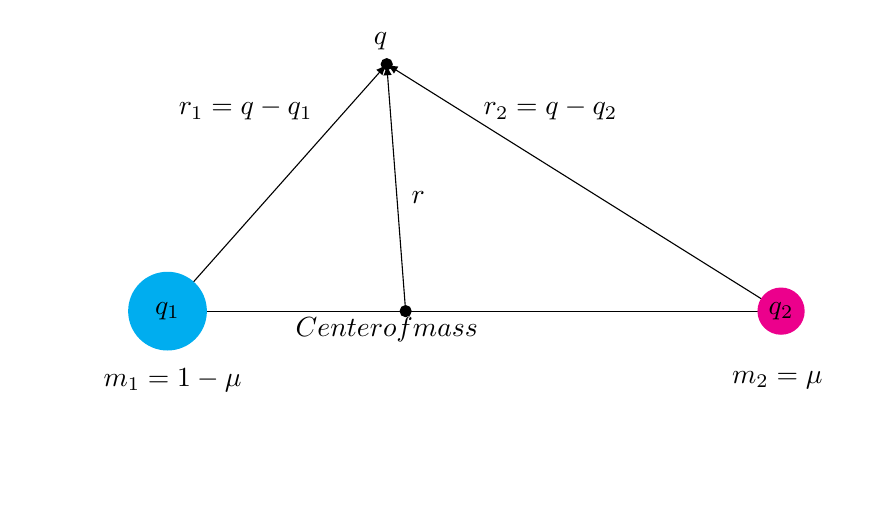
\begin{tikzpicture}[line cap=round,line join=round,x=0.8cm,y=0.8cm]
	\clip(-6,-2.8) rectangle (7,4.5);
	\draw [->] (5.96,-0) -- (-0.3,3.92);
	\draw [->] (-3.78,0) -- (-0.3,3.92);
	\draw (5.96,-0)-- (-3.78,0);
	\draw [->] (0,0) -- (-0.3,3.92);
	\draw[color=black] (-3.7,-1.1) node {$m_1 = 1 - \mu$};
	\draw[color=black] (5.9,-1.1) node {$m_2 = \mu$};
	\draw [fill=black] (-0.3,3.92) circle (2pt);
	\draw [fill=black] (-3.78,0) circle (1.5pt);
	\draw [fill=black] (5.96,-0) circle (1.5pt);
	\draw[color=black] (-0.4,4.29) node {$q$};
	\draw[color=black] (2.3,3.2) node {$r_2 = q - q_2$};
	\draw[color=black] (-2.54,3.2) node {$r_1 = q - q_1 $};
	\draw [fill=black] (0,0) circle (2pt);
	\draw[color=black] (-0.3,-0.3) node {$\text{Center of mass}$};
	\draw[color=black] (0.2,1.8) node {$r$};
	\draw [fill=cyan,draw=none,fill opacity=1] (-3.78,0) circle (0.5cm);
	\draw [fill=magenta,draw=none,fill opacity=1] (5.96,0) circle (0.3cm);
	\draw[color=black] (-3.78,0) node {$q_1$};
	\draw[color=black] (5.96,0) node {$q_2$};
	\end{tikzpicture}
	\caption{Scheme of the three-body problem.}
\end{figure}


As it was observed in \cite{kiesenhofermirandascott}, it is possible to associate a singular structure to this problem. Consider the symplectic form on $\mathrm{T}^{\ast} \mathbb{R}^2$ in polar coordinates,
After making a change to polar coordinates $(q_1,q_2)=(r\cos\alpha,r\sin\alpha)$ and the corresponding canonical change of momenta we find the Hamiltonian function
\begin{equation}
H(r,\alpha,P_r,P_\alpha)=\frac{P_r^2}{2}+\frac{P_\alpha ^2}{2r^2}+U(r\cos\alpha,r\sin\alpha)
\end{equation}
where $P_r,P_\alpha$ are the associated canonical momenta and with potential energy:
$U(r\cos\alpha,r\sin\alpha)$

The McGehee change of coordinates is used to examine the behavior of orbits near infinity, see also \cite{delshams2015global}:
\begin{equation}\label{eqn:McGehee}
r=\frac{2}{x^2}.
\end{equation}
The corresponding change for the canonical momenta is easily seen to be
\begin{equation}
P_r=-\frac{x^3}{4}P_x.
\end{equation}
The Hamiltonian is transformed to
\begin{equation}
H(r,\alpha,P_r,P_\alpha)=\frac{x^6P_x^2}{32}+\frac{x^4P_\alpha^2}{8}+U(x,\alpha).
\end{equation}
By  transforming the position coordinate~(\ref{eqn:McGehee}) without modifying the momentum associated to $r$, we are left with a simpler Hamiltonian, however, the pull-back of the symplectic form  is no longer symplectic, but exhibits a singularity of order $3$ and it is called $b^3$-symplectic:
\begin{equation}
\omega= \frac{4}{x^3} dx \wedge dP_r + d\alpha\wedge d P_\alpha.
\end{equation}

Adding the line at infinity provides a description of the dynamics within the critical set $Z=\{x=0\}$.
From the change of coordinates implemented, we might think that the dynamics within  $Z$ may have  no physical meaning, but its interplay with the dynamics close to $Z$ gives information about the behaviour of escape orbits sometimes identified as \emph{singular periodic orbits} (see \cite{MO20} and \cite{cedricdanieleva}).




Given an autonomous Hamiltonian system of a symplectic manifold  of dimension $2n$, the level sets of the Hamiltonian function are often endowed with a contact structure
( a contact structure is given by a one form $\alpha$ satisfying a condition of type $\alpha\wedge (d\alpha)^{n-1}\neq 0$).

In \cite{MO18, MO20}  applications of the $b$-apparatus are discussed in this context. In particular, the notion of $b^m$-contact structures is introduced by translating the condition above for $b^m$-forms. The classical notions in the contact realm such as  Reeb vector fields can also be introduced in this set-up.

By considering the McGehee change as we did in the contact context,  the following theorem is proved in \cite{MO20}:

\begin{theorem}\label{thm:bcontact3bp}
After the McGehee change, the Liouville vector field $Y=p\frac{\partial}{\partial p}$ is a $b^3$-vector field that is everywhere transverse to the level sets of the Hamiltonian $\Sigma_c$ for $c>0$ and the level-sets $(\Sigma_c,\iota_Y \omega)$ for $c>0$ are $b^3$-contact manifolds. Topologically, the critical set of this contact manifold is a cylinder (which can be interpreted as a subset of the line at infinity) and the Reeb vector field admits infinitely many non-trivial periodic orbits on the critical set.
\end{theorem}



The  KAM theorem in this monograph can be applied to find new periodic orbits of the restricted three-body problem close to infinity by perturbing the periodic orbits described above (see also \cite{MO20}).  This perturbation technique is an old method in perturbation theory, possibly originating from Poincaré himself (known as Poincaré's continuation method, as mentioned in \cite{meyeroffin}).  This paves the way for further research that will be pursued elsewhere.

\section{Escape orbits in Celestial mechanics and Fluid dynamics}
Reeb vector fields and their dynamics are closely related to Beltrami vector fields, which provide stationary solutions of the Euler equations. Indeed, Etnyre and Ghrist \cite{EG} revealed the existence of a "mirror" that reflects Reeb vector fields as Beltrami vector fields. Thus, the applications of KAM theory to find periodic orbits can be exported to understand periodic orbits of stationary fluid flows.  Also, this correspondence yields the possibility to translate concepts in celestial mechanics into  fluid dynamics. Among these concepts is the notion of escape orbits.
The Reeb-Beltrami correspondence was extended to the $b$-setting in \cite{danielevarobert}.

In \cite{MO20} we introduced the notion of singular periodic orbit of a $b$-Reeb vector field $R_{\alpha}$:
\begin{definition}
		Let $(M,\alpha)$ be $b$-contact manifold manifold with critical hypersurface $Z$. Denote by $R_{\alpha}$ its $b$-Reeb vector field.  A \emph{singular periodic orbit} $\gamma$ is an orbit such that $\lim_{t \to  \pm \infty} \gamma(t) =p_{\pm} \in Z$ where $R_{\alpha}(p_{\pm})=0$.
	\end{definition}
	

	
	\begin{figure}[hbt!]\label{fig:singularorbit}
\begin{center}
\begin{tikzpicture}[scale=2.2]
 \draw[color=blue](1,0) arc (0:180:1 and 1);
% \draw (-1,0) -- (1,0);
 \draw[dashed][color=red] (-2,0) --  (2,0);
 \fill (1,0) circle[radius=0.5pt];
 \fill (-1,0) circle[radius=0.5pt];
 %\draw (-0.75,0.2) ..controls +(0,0.5) and +(0,0.5).. node {\midarrow} (0.75,0.2); % arc semicircle up
 %\draw (-0.75,0.2) ..controls +(0,0.3) and +(-0.5,0).. (0,0.7); % arc1 upleft
% \draw (0,0.7) ..controls +(0.5,0) and +(0,0.3).. (0.75,0.2); % arc1 upright
% \draw (-0.75,0.2) ..controls +(0,-0.2) and +(0,-0.2).. (0.75,0.2); %arc1 down
%  \draw (-0.6,0.3) ..controls +(0,0.05) and +(-0.5,0).. (0,0.6); % arc2 upleft
% \draw (0,0.6) ..controls +(0.5,0) and +(0,0.05).. (0.6,0.3); % arc2 upright
% \draw (-0.6,0.3) ..controls +(0,-0.2) and +(0,-0.2).. (0.6,0.3); %arc2 down
%\flecha[shift={(0,0)},black,scale=2,rotate=];
%\fill [shift={(0.05,0)},scale=0.05,rotate=0]   (0,0) -- (-1,-0.7) -- (-1,0.7) -- cycle;
\fill [shift={(-0.05,1)},scale=0.05,rotate=180]   (0,0) -- (-1,-0.7) -- (-1,0.7) -- cycle; %arrow up
%\fill [shift={(-0.05,0.7)},scale=0.05,rotate=180]   (0,0) -- (-1,-0.7) -- (-1,0.7) -- cycle; %arrow up (2nd)
%\fill [shift={(0.05,0.15)},scale=0.05,rotate=0]   (0,0) -- (-1,-0.7) -- (-1,0.7) -- cycle;
%\fill [shift={(0.05,0.24)},scale=0.05,rotate=0]   (0,0) -- (-1,-0.7) -- (-1,0.7) -- cycle;
%  \draw[shift={(0,0.15)},scale=0.6] (-0.6,0.3) ..controls +(0,0.05) and +(-0.5,0).. (0,0.6); % arc2 upleft
% \draw[shift={(0,0.15)},scale=0.6] (0,0.6) ..controls +(0.5,0) and +(0,0.05).. (0.6,0.3); % arc2 upright
% \draw[shift={(0,0.15)},scale=0.6] (-0.6,0.3) ..controls +(0,-0.2) and +(0,-0.2).. (0.6,0.3); %arc2 down
\end{tikzpicture}

\caption{A singular periodic orbit}

\end{center}
\end{figure}

The singular Weinstein conjecture was conjecture in \cite{MO20}. 
In \cite{cedricdanieleva} the existence of  singular periodic orbits  and  generalizations
such as oscillatory motions is investigated for singular structures. Singular periodic orbits are a particular case of escape orbits.




Escape orbits for $b$-Beltrami or $b$-Reeb vector fields, are orbits whose $\alpha$- or $\omega$-limit set lies on the critical set associated to the $b$-structure. The $b$-Reeb Beltrami correspondence together with results of Uhlenbeck \cite{uhlenbeck} on Laplacian eigenfunctions yields that for the majority of asymptotically exact $b$-metrics, $b$-Beltrami vector fields have escape orbits.

 The following theorem proved in \cite{cedricdanielevajosep} gives a lower bound on the number of escape orbits for generic classes of $b$-Beltrami or $b$-Reeb vector fields. The lower bound depends on the number of connected components of the critical set of $Z$ but can often be infinite.

\begin{theorem}{\cite{cedricdanielevajosep}}
    Let $(M,Z)$ be a $3$-dimensional $b$-manifold. Then for a generic asymptotically exact $b$-metric, any $b$-Beltrami vector field has either at least $2N$ or infinitely many escape orbits, where $N$ is the number of connected components of $Z$.
\end{theorem}

In view of the $b$-Reeb-Beltrami correspondence, this implies that generic $b$-Reeb vector fields within a special class of $b$-contact forms also have at least $2N$ or infinitely many escape orbits.

Poincaré continuation method and our KAM results thus can be used to localize the singular counterparts or periodic orbits, either escape orbits or singular periodic orbits in these new scenarios described in \cite{eva}, \cite{MO20},\cite{cedricdanieleva}, and \cite{cedricdanielevajosep}.
\endinput

%-----------------------------------------------------------------------
% End of chap1.tex
%-----------------------------------------------------------------------
